% arara: makeindex

% Template for IEEE papers
%% bare_conf.tex
%% V1.4b
%% 2015/08/26
%% by Michael Shell
%% See:
%% http://www.michaelshell.org/
%% for current contact information.
%%
%% This is a skeleton file demonstrating the use of IEEEtran.cls
%% (requires IEEEtran.cls version 1.8b or later) with an IEEE
%% conference paper.
%%
%% Support sites:
%% http://www.michaelshell.org/tex/ieeetran/
%% http://www.ctan.org/pkg/ieeetran
%% and
%% http://www.ieee.org/

%%*************************************************************************
%% Legal Notice:
%% This code is offered as-is without any warranty either expressed or
%% implied; without even the implied warranty of MERCHANTABILITY or
%% FITNESS FOR A PARTICULAR PURPOSE!
%% User assumes all risk.
%% In no event shall the IEEE or any contributor to this code be liable for
%% any damages or losses, including, but not limited to, incidental,
%% consequential, or any other damages, resulting from the use or misuse
%% of any information contained here.
%%
%% All comments are the opinions of their respective authors and are not
%% necessarily endorsed by the IEEE.
%%
%% This work is distributed under the LaTeX Project Public License (LPPL)
%% ( http://www.latex-project.org/ ) version 1.3, and may be freely used,
%% distributed and modified. A copy of the LPPL, version 1.3, is included
%% in the base LaTeX documentation of all distributions of LaTeX released
%% 2003/12/01 or later.
%% Retain all contribution notices and credits.
%% ** Modified files should be clearly indicated as such, including  **
%% ** renaming them and changing author support contact information. **
%%*************************************************************************


% *** Authors should verify (and, if needed, correct) their LaTeX system  ***
% *** with the testflow diagnostic prior to trusting their LaTeX platform ***
% *** with production work. The IEEE's font choices and paper sizes can   ***
% *** trigger bugs that do not appear when using other class files.       ***                          ***
% The testflow support page is at:
% http://www.michaelshell.org/tex/testflow/

\documentclass{book}
\usepackage[quiet]{fontspec}
\usepackage[table,xcdraw,dvipsnames]{xcolor} % Used by spritegrid and others.
\usepackage[obeyspaces,spaces]{url}
\usepackage{longtable}
\usepackage{arydshln}
\usepackage{booktabs}
\usepackage{afterpage}
\usepackage{flushend}
\usepackage{titletoc}
\usepackage[toc]{appendix}
\usepackage{parskip}
\usepackage{graphicx,wrapfig}
\usepackage{float}
\usepackage{caption}
\usepackage{pdfpages}
\usepackage{tikzpagenodes}
\usepackage{imakeidx}
\usepackage[pagestyles,raggedright]{titlesec}
\usepackage[all]{nowidow}
\usepackage[bookmarks=true]{hyperref}
\usepackage{aeb-minitoc}
\usepackage{fix-cm}
\usepackage{textpos}
\usepackage{enumitem}
\usepackage{tcolorbox}
\tcbuselibrary{listings}
%\usepackage{wrapfig}
\usepackage{needspace}
\usepackage{verbatim}
\usepackage{ean13isbn}
\usepackage{setspace}

% Use CHAPTER-PAGE page numbering to make it easier to modify chapters
% later, without messing up page number of the rest of the book.
\usepackage[auto]{chappg}

% Allow cross-references between the various books to the big The MEGA65 Book
\usepackage{xr}
\usepackage{varioref}
\usepackage{xparse}
\externaldocument[M65Book-]{mega65-book}
% And a \ref alternative that checks if it needs to be a cross-reference to the
% MEGA65 Book instead.
\makeatletter
\newcommand{\bookref}[1]{%
    \@ifundefined{r@#1}{%
      {\em the MEGA65 Book}, \nameref{M65Book-#1} (\autoref{M65Book-#1})}{\autoref{#1}}%
}
\newcommand{\bookvref}[1]{%
    \@ifundefined{r@#1}{%
      {\em the MEGA65 Book}, \nameref{M65Book-#1} (\autoref{M65Book-#1})}{Chapter/Appendix \vref{#1}}%
}
\makeatother

% For fixed-width columns in register maps
\usepackage{array}

% Makes tables with double-ruled lines look better
\usepackage{hhline}

% Makes better use of space for reference tables in appendix
\usepackage{multicol}

% Shaded tables with alternate rows colored for better legibility
% Best used with larger tables rather than small tables
\usepackage{colortbl}
\usepackage{adjustbox}
\usepackage[strict]{changepage}

% \makecell command for forcing line breaks in table cells
\usepackage{makecell}

\newcolumntype{L}[1]{>{\raggedright\let\newline\\\arraybackslash\hspace{0pt}}m{#1}}
\newcolumntype{C}[1]{>{\centering\let\newline\\\arraybackslash\hspace{0pt}}m{#1}}
\newcolumntype{R}[1]{>{\raggedleft\let\newline\\\arraybackslash\hspace{0pt}}m{#1}}

% For displaying Letter keys and the MEGA key
% This is a `keys' element for displaying a Mega65 keyboard key
% using a black filled label with rounded edges.
% In order to display a key as a title, use:
%
%     \megakey[title]{Run/Stop}
%
% For displaying a key as a part of the normal document flow, simply use:
%
%    \megakey{Shift}
%
%
% If you get warnings on special characters, mathematical characters etc, use $, eg:
%
%    \megakey{$\leftarrow$}
%
% Other sizes are supported, as part of tcolorbox:
% http://mirror.aarnet.edu.au/pub/CTAN/macros/latex/contrib/tcolorbox/tcolorbox.pdf#subsubsection.4.7.5 however, only `title' and the default: `small' are proposed for use in this manual.
%
% The second macro available here is the megasymbolkey.
% This will display the MEGA symbol as white on a black key box. Simply use:
%
%		 \megasymbolkey
%

\usepackage{tcolorbox}

\newtcbox{\megakeyinner}[1][small]{colback=black, coltext=white, size=#1, fontupper=\bfseries, nobeforeafter,box align=bottom,baseline=3pt,text height=7pt}
\newcommand{\megakey}[2][small]{\megakeyinner[#1]{\uppercase{#2}}}

\newtcbox{\megasymbolkeyinner}{colback=black, coltext=white, clip title=false. fontupper=\symbolfont, box align=bottom,baseline=3pt,text height=7pt}
\newcommand{\megasymbolkey}{\megakeyinner{\megasymbol[white]}\ }


% For displaying print versions petscii character symbols
% This is a collection of symbol macros element for displaying a printed version of the
% MEGA65 graphic characters, as opposed to the bitmap versions in the mega40/80.ttf fonts files.
% You can display characters using the graphicsymbol macro:
%
%    \graphicsymbol{\textcolor{red}{qQ} wWUcbdhjI \textcolor{blue}{JK}}
%
% Or you can, simply use the font itself:
%
%    \begin{symbolfont}%
%	   qQwWeErRtTyYuUiIoOpP\\
%		 aAsSdDfFgGhHjJkKlL\\
%		 zZxXcCvVbBnNmM%
%		 \end{symbolfont}%
%
%
% You can display the MEGA symbol using:
%
%    \megasymbol
%
% This will display the symbol in black. Other colours can be specified by passing them in, for example:
%
% 	 \megasymbol[black]
%		 \megasymbol[white]
%		 \megasymbol[orange]
%		 \megasymbol[blue]
%
% NOTE:
% For using the MEGA symbol in a key, see the \megasymbolkey macro in the keys.txt file.

\usepackage{tcolorbox}

\newcommand{\graphicsymbol}[1]{%
\begin{symbolfont}%
#1
\end{symbolfont}%
}%

\newcommand{\megasymbol}[1][black]{%
\begin{symbolfont}%
\textcolor{#1}{`}%
\end{symbolfont}%
\
}%


% For Mega65 display of code, listings and screen activity
% This is an element for displaying output from the Mega65 screen.
% It can display program code or to show activity on the screen.
% Example of use:
%
%    \begin{screenoutput}
%    10 OPEN 1,8,0,"$0:*,P,R
%    20 : IF DS THEN PRINT DS$: GOTO 100
%    30 GET#1,X$,X$
%    40 DO
%    50 : GET#1,X$,X$: IF ST THEN EXIT
%    60 : GET#1,BL$,BH$
%    70 : LINE INPUT#1, F$
%    80 : PRINT LEFT$(F$,18)
%    90 LOOP
%    100 CLOSE 1
%
%    RUN
%    \end{screenoutput}

\usepackage{listings,color}

\lstnewenvironment{screenoutput}
   {
     \lstset{
               basicstyle=\codefont\color{white}\linespread{1.1}\normalsize,
               backgroundcolor=\color{black},fillcolor=\color{black},
               frame=lines,
               rulecolor=\color{white},
               framexleftmargin=2mm,
               framexrightmargin=2mm,
               framextopmargin=2mm,
               framexbottommargin=2mm,
               tabsize=4,
               xleftmargin=2mm,
               xrightmargin=2mm,
               basewidth={0.4em},
               escapeinside={\%*}{*\%},
               literate={\*}{*}1{\-}{-}1{\/}{/}1{{\ }}{{ }}1
            }
   }
   {  }


% For in-line screen text
\newcommand{\screentext}[1]{ {\codefont\color{black}\normalsize{#1}} }



% For MEGA65 screen shots with text flow
\newcommand{\screenshotwrap}[1]{{\begin{center}\includegraphics[width=0.80\linewidth]{#1}\end{center}}}
%\newcommand{\screenshotwrap}[1]{\needspace{8cm}\setlength{\intextsep}{0pt}\begin{wrapfigure}{i}{0.80\textwidth}\includegraphics[width=\linewidth]{#1}\end{wrapfigure}}


% For displaying sprite data in a grid
% This is an element for displaying a sprite in a grid, just like page 70 of the
% commodore manual. This version can be easily expanded. For now it will suffice.
% In order to display a hi-res mono sprite grid use:
%
%	\spritegrid{
%	\hline
%	\spritecells{---------ooooo----------}
%	\spritecells{-------ooooooooo--------}
%	\spritecells{------ooooooooooo-------}
%	\spritecells{------ooo--o---oo-------}
%	\spritecells{-----ooo-ooo-ooooo------}
%	\spritecells{-----ooo-ooo-ooooo------}
%	\spritecells{-----ooo---o---ooo------}
%	\spritecells{-----ooo-o-ooo-ooo------}
%	\spritecells{-----ooo-o-ooo-ooo------}
%	\spritecells{-----ooo---o--oooo------}
%	\spritecells{------ooooooooooo-------}
%	\spritecells{------ooooooooooo-------}
%	\spritecells{-------ooooooooo--------}
%	\spritecells{-------o-ooooo-o--------}
%	\spritecells{--------o-o-o-o---------}
%	\spritecells{--------o--o--o---------}
%	\spritecells{---------o-o-o----------}
%	\spritecells{---------o-o-o----------}
%	\spritecells{---------ooooo----------}
%	\spritecells{---------ooooo----------}
%	\spritecells{----------ooo-----------}
%	}
%
% For a multicolour sprite:
%
%	\spritegrid{
%	\hline
%	\spritecells{------------------------}
%	\spritecells{------------------------}
%	\spritecells{------------------------}
%	\spritecells{------------------------}
%	\spritecells{--------llllll----------}
%	\spritecells{------llllllggll--------}
%	\spritecells{------llllllllgg--------}
%	\spritecells{----llllllgggggggg------}
%	\spritecells{----llllggeeeellll------}
%	\spritecells{----lloollllllggee------}
%	\spritecells{----llooggggooggee------}
%	\spritecells{----llooggggooggee------}
%	\spritecells{----eeeeggggooeeee------}
%	\spritecells{----ggeeeeeeeeoo--------}
%	\spritecells{------ggooooooee--------}
%	\spritecells{------eeggeeeeee--------}
%	\spritecells{--------eeeeee----------}
%	\spritecells{------------------------}
%	\spritecells{------------------------}
%	\spritecells{------------------------}
%	\spritecells{------------------------}
%	}

\usepackage{tabulary} %Removes spacing from tabulars
\usepackage{xstring} % for string substitution
\usepackage{xparse} % used for unpacking the sprite characters
% \renewcommand{\familydefault}{\sfdefault} % default sans font

%\usepackage{graphicx} % for resizing the tabular used by spritegrid
\usepackage{subcaption} % used for the left hand subtable of row numbers
\usepackage{multirow} % used for the ``Row'' column
\usepackage{rotating} % used by the rotating ``Row'' word

\newcommand{\spritebytecolumn}[1]{
   %\framebox[4mm]{#1}
   \makebox[4mm]{#1}
}

\setlength\tabcolsep{0.3mm} % the indivdual cell width and height


% Cell colour list. Can be expanded for other colours in the sprite grid
\def\blk{\cellcolor{black}}
\def\wht{\cellcolor{white}}
\def\grn{\cellcolor{ForestGreen}}
\def\lgrn{\cellcolor{YellowGreen}}
\def\gry{\cellcolor{Gray}}

\newcounter{lettercounter} % counter for detecting the last cell

% Collect the spritecell list and send it to \ProcessSpriteCell for turning into cells
\NewDocumentCommand{\spritecells}{%
>{\SplitList{}} m }{%
  \ProcessList{#1}{\ProcessSpriteCell}%
}

\NewDocumentCommand{\ProcessSpriteCell}{m}{%
  \stepcounter{lettercounter}%
    \IfStrEqCase{#1}{
	{o}{\blk}
	{-}{\wht}
	{g}{\grn}
	{l}{\lgrn}
	{e}{\gry}
   }%
   \IfStrEq{\thelettercounter}{24}{\setcounter{lettercounter}{0} \\ \hline}{&}%
}

% Start of the actual spritegrid definition
\newcommand{\spritegrid}[1]{
\begin{table}[h!]
\centering
\begin{subtable}{28mm}
\vspace{8mm}
\scalebox{0.76}{
\begin{tabular}{p{25mm} p{4mm} c}
\multirow{21}{*}{ } &
\multirow{21}{*}{%
\begin{turn}{90}%
\bfseries\uppercase{Row}%
\end{turn}} &
 1\\
& & 2\\
& & 3\\
& & 4\\
& & 5\\
& & 6\\
& & 7\\
& & 8\\
& & 9\\
& & 10\\
& & 11\\
& & 12\\
& & 13\\
& & 14\\
& & 15\\
& & 16\\
& & 17\\
& & 18\\
& & 19\\
& & 20\\
& & 21
\end{tabular}
}
\end{subtable}%
\begin{subtable}{.8\textwidth}

\setlength{\arrayrulewidth}{1pt}
\scalebox{0.7}{
\begin{tabular}{  *{3}{p{30mm} }  }
  \center\uppercase{Series\\1} &
  \center\uppercase{Series\\2} &
  \center\uppercase{Series\\3}
\end{tabular}
}

\scalebox{0.7}{
\begin{tabular}{p{5.8mm} *{11}{C{7.3mm}}}
   128 & 32 & 8 & 2 & 128 & 32 & 8 & 2 & 128 & 32 & 8 & 2
\end{tabular}
}
\\[-1.5mm]
\scalebox{0.7}{
\begin{tabular}{p{1.7mm} *{12}{C{7.3mm}}}
  & 64 & 16 & 4 & 1 & 64 & 16 & 4 & 1 & 64 & 16 & 4 & 1
\end{tabular}
}

\scalebox{0.7}{
\begin{tabular}{ | *{24}{p{3mm} |}  }
#1
\end{tabular}
}

\scalebox{0.7}{
\begin{tabular}{ *{24}{p{3.35mm}}  }
	\spritebytecolumn{1} & & & &
	\spritebytecolumn{5} & & & & &
	\spritebytecolumn{10} & & & & &
	\spritebytecolumn{15} & & & & &
	\spritebytecolumn{20} & & & &
	\spritebytecolumn{24} \\
	\multicolumn{24}{c}{\bfseries\uppercase{Column}}
\end{tabular}
}
\end{subtable}
\end{table}
}

% End of the actual spritegrid definition



% Don't number sections
\setcounter{secnumdepth}{0}

\renewcommand{\indexname}{INDEX}
\renewcommand{\appendixtocname}{APPENDICES}
\renewcommand{\appendixpagename}{APPENDICES}
\renewcommand{\appendixpage}{%
  \clearpage\thispagestyle{empty}
    \pagecolor{blue}
     \begin{center}
       {
         \large
         % Put a nice amount of vertical space before the title
         \vspace*{2cm}
               {\large\Huge\textcolor{white}{\bf{APPENDICES}}}\\
             \vspace{\fill}
       }
     \end{center}
     \newpage\pagecolor{white}\clearpage
}

\makeatletter\chardef\pdf@shellescape=\@ne\makeatother

\setcounter{tocdepth}{5}

% 1.0 cm is the distance from left of page to bullet point.
% 2.8 cm is a fudge-factor to make multi-line section names be correctly lined up.
% \@B{〈length〉} is the amount to indent prior to〈sec-num >
% \@F{〈fmt〉} is the formatting for the title heading
% \@P{〈fmt〉} is the formatting for the page number (〈pg-num〉).

\TOCLevels{chapter}{section}
\begin{minitocfmt}{\chapmtoc}
\declaretocfmt{section}{\@F{\color{white}\hspace{1.0cm}\textbullet\hspace{0.25cm}\Large\bfseries}\@B{2.8cm}\@P{\mtocgobble}}
\declaretocfmt{section*}{\@F{\color{white}\hspace{1.0cm}\textbullet\hspace{0.25cm}\Large\bfseries}\@B{2.8cm}\@P{\mtocgobble}}
\end{minitocfmt}

\usepackage{fontspec}

\setmainfont[Path=fonts/, BoldFont=MegaGlacial-Bold.otf, ItalicFont=MegaGlacial-Italic.otf]{MegaGlacial-Regular.otf}
%\setmainfont[Path=fonts/, BoldFont=GlacialIndifference-Bold.otf, ItalicFont=GlacialIndifference-Italic.otf]{GlacialIndifference-Regular.otf}
\newfontfamily\serifed[Path=fonts/, BoldFont=xits-bold.otf, ItalicFont=xits-italic.otf]{xits-regular.otf}
\newfontface\codefont[Path=fonts/]{mega80.ttf}
\newfontface\symbolfont[Path=fonts/]{MEGA65GraphicSymbols.otf}


% Set margins for inner and outer pages in A5 book format
\ifdefined\printmanual
\usepackage[a5paper,nomarginpar,includemp,bottom=2cm,top=1cm,inner=1.8cm,outer=0.8cm, footskip = 1cm]{geometry}
\else
\usepackage[a5paper,nomarginpar,includemp,bottom=2cm,top=1cm,inner=1.0cm,outer=1.0cm, footskip = 1cm]{geometry}
\fi

% Some Computer Society conferences also require the compsoc mode option,
% but others use the standard conference format.
%
% If IEEEtran.cls has not been installed into the LaTeX system files,
% manually specify the path to it like:
% \documentclass[conference]{../sty/IEEEtran}

%% % Some very useful LaTeX packages include:

% *** MISC UTILITY PACKAGES ***
%
%\usepackage{ifpdf}
% Heiko Oberdiek's ifpdf.sty is very useful if you need conditional
% compilation based on whether the output is pdf or dvi.
% usage:
% \ifpdf
%   % pdf code
% \else
%   % dvi code
% \fi
% The latest version of ifpdf.sty can be obtained from:
% http://www.ctan.org/pkg/ifpdf
% Also, note that IEEEtran.cls V1.7 and later provides a builtin
% \ifCLASSINFOpdf conditional that works the same way.
% When switching from latex to pdflatex and vice-versa, the compiler may
% have to be run twice to clear warning/error messages.



\usepackage{csquotes}


% *** CITATION PACKAGES ***
%
\usepackage{cite}
% cite.sty was written by Donald Arseneau
% V1.6 and later of IEEEtran pre-defines the format of the cite.sty package
% \cite{} output to follow that of the IEEE. Loading the cite package will
% result in citation numbers being automatically sorted and properly
% "compressed/ranged". e.g., [1], [9], [2], [7], [5], [6] without using
% cite.sty will become [1], [2], [5]--[7], [9] using cite.sty. cite.sty's
% \cite will automatically add leading space, if needed. Use cite.sty's
% noadjust option (cite.sty V3.8 and later) if you want to turn this off
% such as if a citation ever needs to be enclosed in parenthesis.
% cite.sty is already installed on most LaTeX systems. Be sure and use
% version 5.0 (2009-03-20) and later if using hyperref.sty.
% The latest version can be obtained at:
% http://www.ctan.org/pkg/cite
% The documentation is contained in the cite.sty file itself.






% *** GRAPHICS RELATED PACKAGES ***
%
\ifCLASSINFOpdf
   \usepackage[pdftex]{graphicx}
  % declare the path(s) where your graphic files are
   \graphicspath{{../pdf/}{../jpeg/}}
  % and their extensions so you won't have to specify these with
  % every instance of \includegraphics
   \DeclareGraphicsExtensions{.pdf,.jpeg,.png}
\else
  % or other class option (dvipsone, dvipdf, if not using dvips). graphicx
  % will default to the driver specified in the system graphics.cfg if no
  % driver is specified.
   \usepackage[dvips]{graphicx}
  % declare the path(s) where your graphic files are
%   \graphicspath{{../eps/}}
  % and their extensions so you won't have to specify these with
  % every instance of \includegraphics
   \DeclareGraphicsExtensions{.eps}
\fi
% graphicx was written by David Carlisle and Sebastian Rahtz. It is
% required if you want graphics, photos, etc. graphicx.sty is already
% installed on most LaTeX systems. The latest version and documentation
% can be obtained at: 
% http://www.ctan.org/pkg/graphicx
% Another good source of documentation is "Using Imported Graphics in
% LaTeX2e" by Keith Reckdahl which can be found at:
% http://www.ctan.org/pkg/epslatex
%
% latex, and pdflatex in dvi mode, support graphics in encapsulated
% postscript (.eps) format. pdflatex in pdf mode supports graphics
% in .pdf, .jpeg, .png and .mps (metapost) formats. Users should ensure
% that all non-photo figures use a vector format (.eps, .pdf, .mps) and
% not a bitmapped formats (.jpeg, .png). The IEEE frowns on bitmapped formats
% which can result in "jaggedy"/blurry rendering of lines and letters as
% well as large increases in file sizes.
%
% You can find documentation about the pdfTeX application at:
% http://www.tug.org/applications/pdftex





% *** MATH PACKAGES ***
%
%\usepackage{amsmath}
% A popular package from the American Mathematical Society that provides
% many useful and powerful commands for dealing with mathematics.
%
% Note that the amsmath package sets \interdisplaylinepenalty to 10000
% thus preventing page breaks from occurring within multiline equations. Use:
%\interdisplaylinepenalty=2500
% after loading amsmath to restore such page breaks as IEEEtran.cls normally
% does. amsmath.sty is already installed on most LaTeX systems. The latest
% version and documentation can be obtained at:
% http://www.ctan.org/pkg/amsmath





% *** SPECIALIZED LIST PACKAGES ***
%
%\usepackage{algorithmic}
% algorithmic.sty was written by Peter Williams and Rogerio Brito.
% This package provides an algorithmic environment fo describing algorithms.
% You can use the algorithmic environment in-text or within a figure
% environment to provide for a floating algorithm. Do NOT use the algorithm
% floating environment provided by algorithm.sty (by the same authors) or
% algorithm2e.sty (by Christophe Fiorio) as the IEEE does not use dedicated
% algorithm float types and packages that provide these will not provide
% correct IEEE style captions. The latest version and documentation of
% algorithmic.sty can be obtained at:
% http://www.ctan.org/pkg/algorithms
% Also of interest may be the (relatively newer and more customizable)
% algorithmicx.sty package by Szasz Janos:
% http://www.ctan.org/pkg/algorithmicx




% *** ALIGNMENT PACKAGES ***
%
%\usepackage{array}
% Frank Mittelbach's and David Carlisle's array.sty patches and improves
% the standard LaTeX2e array and tabular environments to provide better
% appearance and additional user controls. As the default LaTeX2e table
% generation code is lacking to the point of almost being broken with
% respect to the quality of the end results, all users are strongly
% advised to use an enhanced (at the very least that provided by array.sty)
% set of table tools. array.sty is already installed on most systems. The
% latest version and documentation can be obtained at:
% http://www.ctan.org/pkg/array


% IEEEtran contains the IEEEeqnarray family of commands that can be used to
% generate multiline equations as well as matrices, tables, etc., of high
% quality.

%%%%%%%%%%%%%%%%%
\usepackage{multirow}
\usepackage[table]{xcolor}
\usepackage{tablefootnote}
\usepackage[bottom]{footmisc}

%%%%%%%%%%%%%%%%%%

% *** SUBFIGURE PACKAGES ***
\ifCLASSOPTIONcompsoc
  \usepackage[caption=false,font=normalsize,labelfont=sf,textfont=sf]{subfig}
\else
  \usepackage[caption=false,font=footnotesize]{subfig}
\fi
% subfig.sty, written by Steven Douglas Cochran, is the modern replacement
% for subfigure.sty, the latter of which is no longer maintained and is
% incompatible with some LaTeX packages including fixltx2e. However,
% subfig.sty requires and automatically loads Axel Sommerfeldt's caption.sty
% which will override IEEEtran.cls' handling of captions and this will result
% in non-IEEE style figure/table captions. To prevent this problem, be sure
% and invoke subfig.sty's "caption=false" package option (available since
% subfig.sty version 1.3, 2005/06/28) as this is will preserve IEEEtran.cls
% handling of captions.
% Note that the Computer Society format requires a larger sans serif font
% than the serif footnote size font used in traditional IEEE formatting
% and thus the need to invoke different subfig.sty package options depending
% on whether compsoc mode has been enabled.
%
% The latest version and documentation of subfig.sty can be obtained at:
% http://www.ctan.org/pkg/subfig




% *** FLOAT PACKAGES ***
%
%\usepackage{fixltx2e}
% fixltx2e, the successor to the earlier fix2col.sty, was written by
% Frank Mittelbach and David Carlisle. This package corrects a few problems
% in the LaTeX2e kernel, the most notable of which is that in current
% LaTeX2e releases, the ordering of single and double column floats is not
% guaranteed to be preserved. Thus, an unpatched LaTeX2e can allow a
% single column figure to be placed prior to an earlier double column
% figure.
% Be aware that LaTeX2e kernels dated 2015 and later have fixltx2e.sty's
% corrections already built into the system in which case a warning will
% be issued if an attempt is made to load fixltx2e.sty as it is no longer
% needed.
% The latest version and documentation can be found at:
% http://www.ctan.org/pkg/fixltx2e


%\usepackage{stfloats}
% stfloats.sty was written by Sigitas Tolusis. This package gives LaTeX2e
% the ability to do double column floats at the bottom of the page as well
% as the top. (e.g., "\begin{figure*}[!b]" is not normally possible in
% LaTeX2e). It also provides a command:
%\fnbelowfloat
% to enable the placement of footnotes below bottom floats (the standard
% LaTeX2e kernel puts them above bottom floats). This is an invasive package
% which rewrites many portions of the LaTeX2e float routines. It may not work
% with other packages that modify the LaTeX2e float routines. The latest
% version and documentation can be obtained at:
% http://www.ctan.org/pkg/stfloats
% Do not use the stfloats baselinefloat ability as the IEEE does not allow
% \baselineskip to stretch. Authors submitting work to the IEEE should note
% that the IEEE rarely uses double column equations and that authors should try
% to avoid such use. Do not be tempted to use the cuted.sty or midfloat.sty
% packages (also by Sigitas Tolusis) as the IEEE does not format its papers in
% such ways.
% Do not attempt to use stfloats with fixltx2e as they are incompatible.
% Instead, use Morten Hogholm'a dblfloatfix which combines the features
% of both fixltx2e and stfloats:
%
% \usepackage{dblfloatfix}
% The latest version can be found at:
% http://www.ctan.org/pkg/dblfloatfix


% *** PDF, URL AND HYPERLINK PACKAGES ***
%
\usepackage{url}
% url.sty was written by Donald Arseneau. It provides better support for
% handling and breaking URLs. url.sty is already installed on most LaTeX
% systems. The latest version and documentation can be obtained at:
% http://www.ctan.org/pkg/url
% Basically, \url{my_url_here}.


% *** Do not adjust lengths that control margins, column widths, etc. ***
% *** Do not use packages that alter fonts (such as pslatex).         ***
% There should be no need to do such things with IEEEtran.cls V1.6 and later.
% (Unless specifically asked to do so by the journal or conference you plan
% to submit to, of course. )


% *** Use glossaries for abbreviations ***
\usepackage[acronym, nowarn]{glossaries}
\makeglossaries
%!TEX root = pairing.tex
% ********************************************************************
% Definition of acronyms
% ********************************************************************
% Specify new acronyms using the following command:
% 	\newacronym{<label>}{<abbrv>}{<full>}
%
% Using acronyms in text is supported by using 
% 	\gls  	This command prints the term associated with <label>
% 	\glspr 	This command prints the plural of the defined term
% 	\Gls 	This command prints the singular form with the first character
%				converted to upper case.
% 	\Glspl Upercase, Plural

\newacronym{manet}{\textsc{MANET}}{mobile ad hoc networks}
\newacronym{tetra}{\textsc{TETRA}}{Terrestrial Trunked Radio}
\newacronym{hf}{\textsc{HF}}{High Frequency}
\newacronym{uhf}{\textsc{UHF}}{Ultra High Frequency}
\newacronym{vhf}{\textsc{VHF}}{Very High Frequency}
\newacronym{sbd}{\textsc{SBD}}{short-burst-data}

% *** Use SI Units
\usepackage[binary-units=true]{siunitx}
\sisetup{per-mode = symbol,
		 list-final-separator = {, and},
		 range-phrase = \ {;}\ ,
		 range-units  = brackets,
		 open-bracket = [,
	     close-bracket= ],}


% correct bad hyphenation here
\hyphenation{op-tical net-works semi-conduc-tor}

\makeindex[intoc]

\pagestyle{empty}

\begin{document}
\raggedbottom

% relax word wrapping with sloppy
\sloppy
% reduce overfull \hbox warnings
\hfuzz=5pt

% macro for changing the verbatim font
\makeatletter
\newcommand{\verbatimfont}[1]{\def\verbatim@font{#1}}%
\makeatother



%\pagecolor{blue}
%\clearpage\thispagestyle{empty}
%\begin{center}
%
\includegraphics[width=\textwidth]{frontcover/MEGA65_logo_shadow}
%
%{\textcolor{white}{\large\Huge{\bf{USER'S GUIDE}}}}
%
%\vspace{\fill}
%       {\textcolor{white}{\large\huge{Museum of Electronic Games and Art (M.E.G.A.)}}}
%\end{center}
%
\begin{tikzpicture}[remember picture,overlay,shift={(current page.north east)}]
\node[anchor=north east,xshift=0.2cm,yshift=0.1cm]{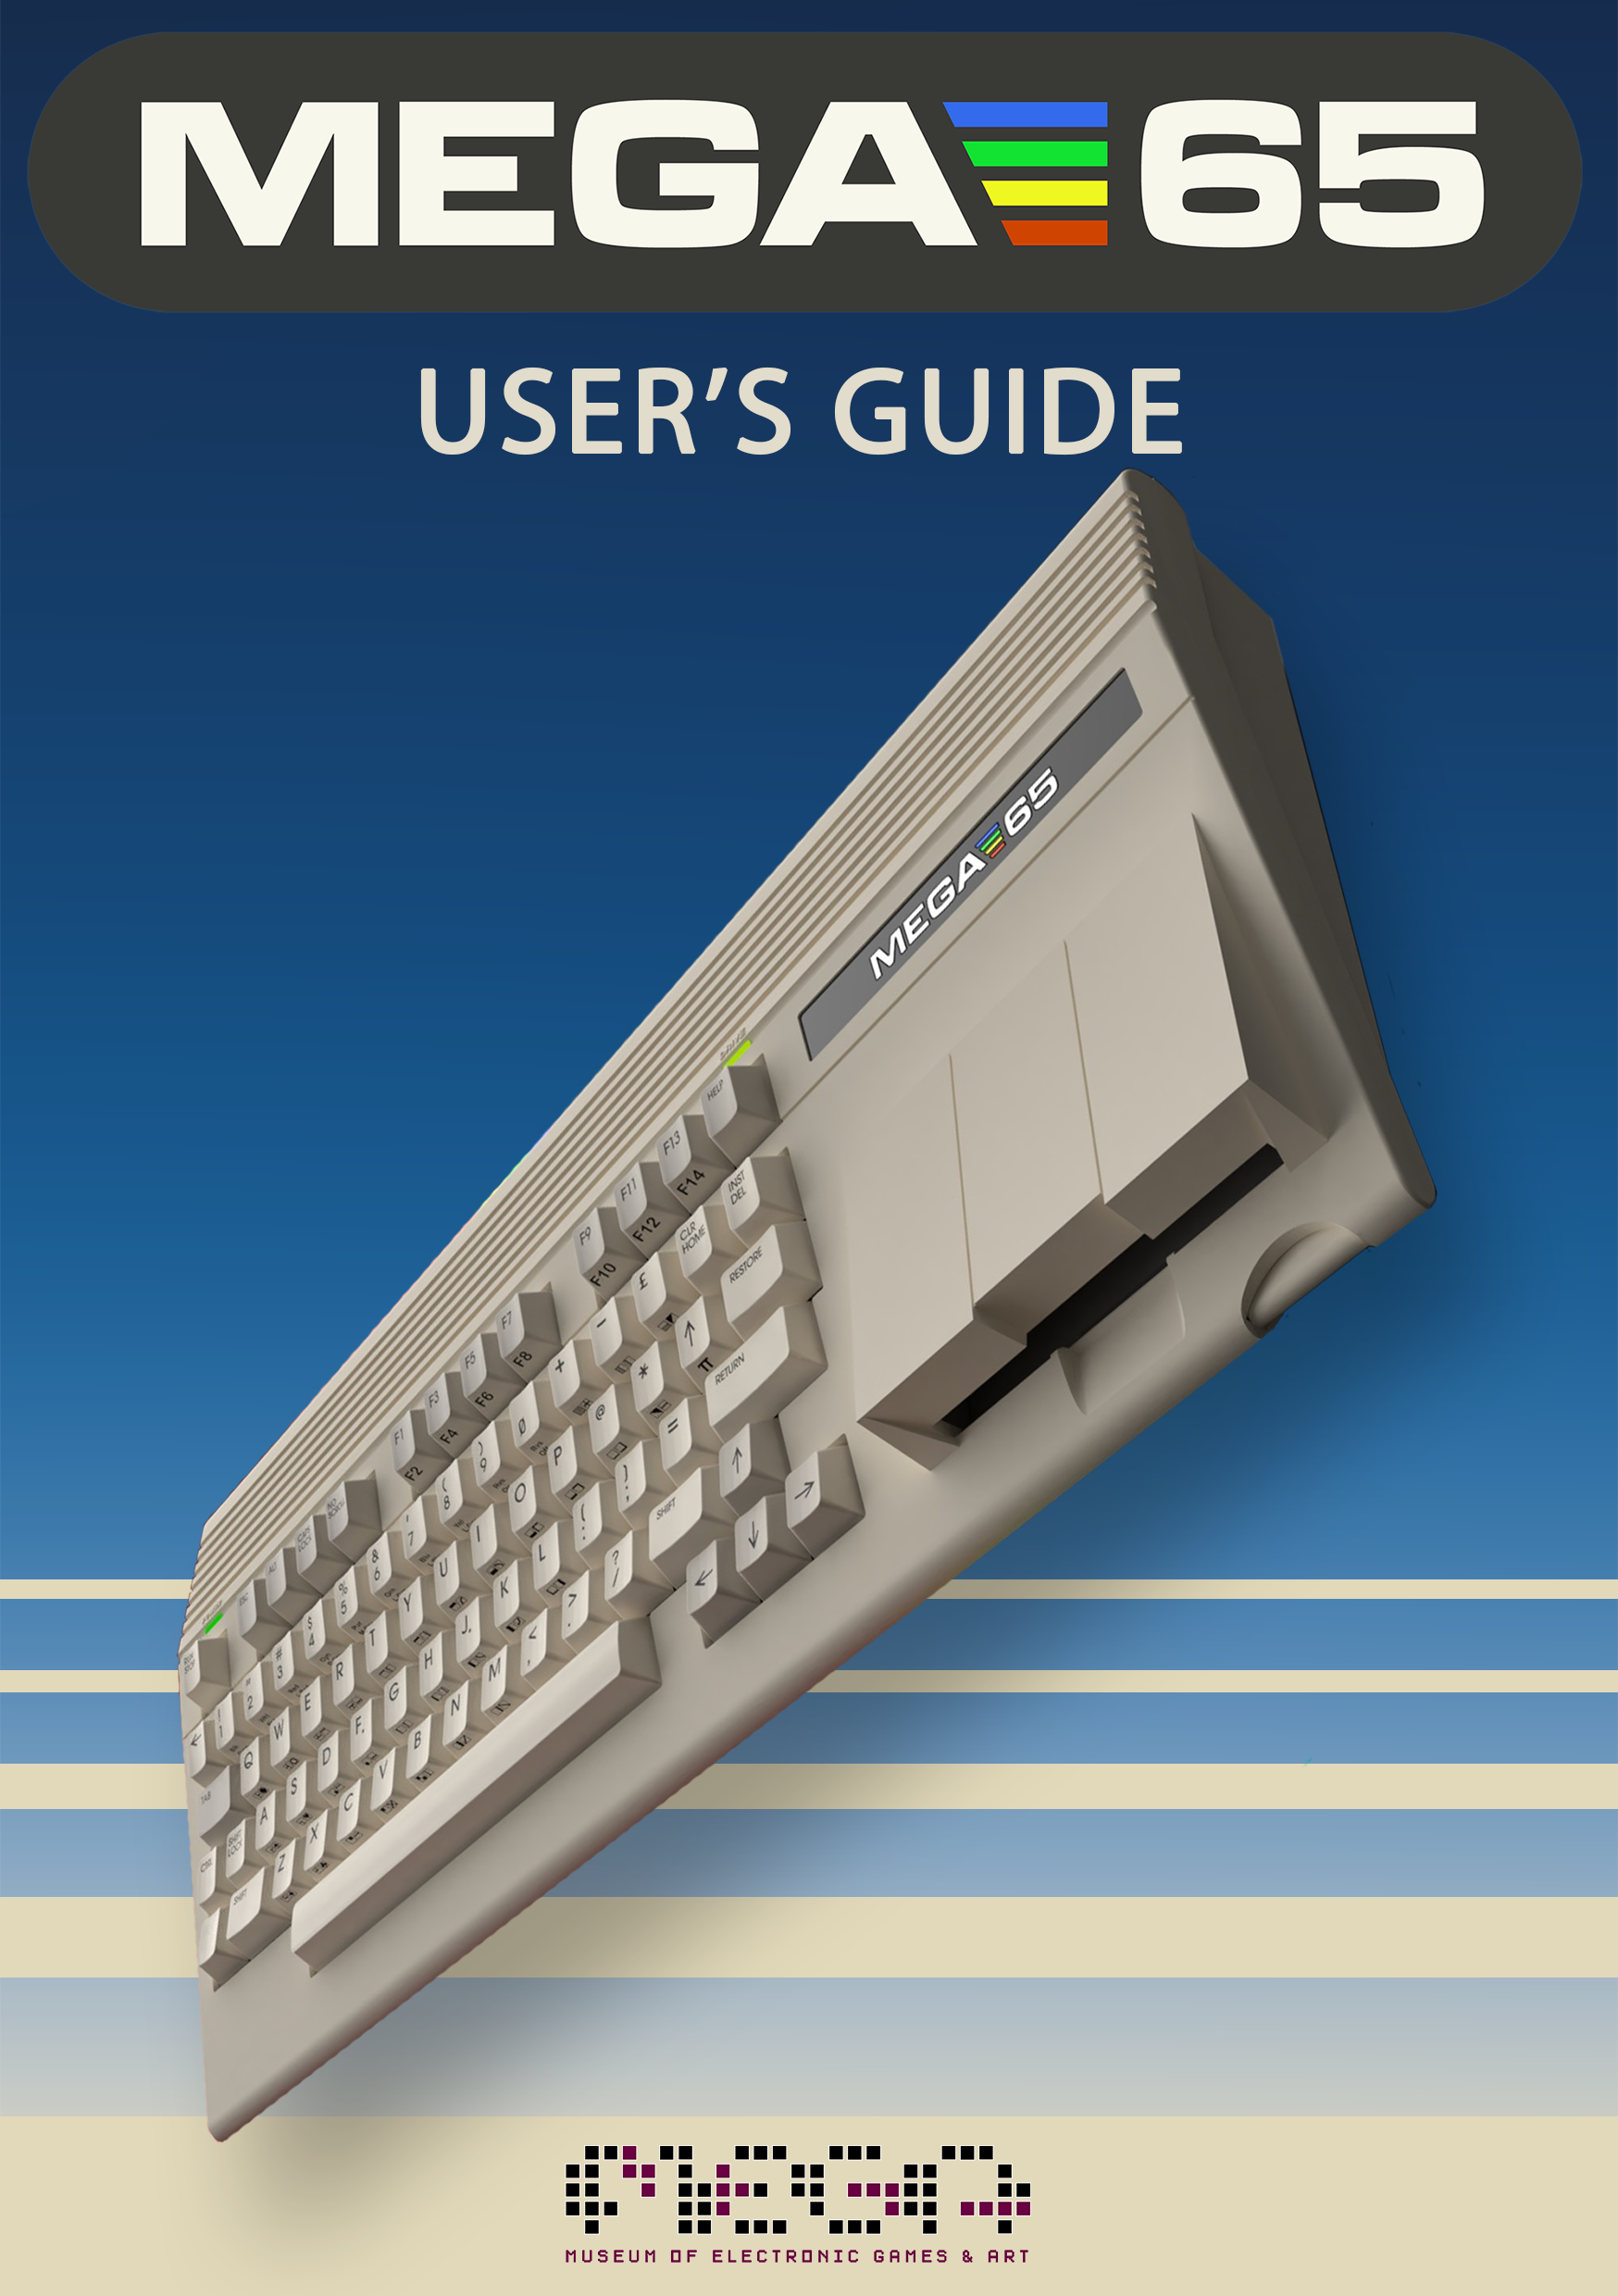
\includegraphics[height=210mm,width=149mm]{frontcover/manual_title}};
\end{tikzpicture}

%\newpage
%\pagecolor{white}

%\vspace*{-2cm}\chapter*{MEGA65 TEAM}
\newpage
{\huge MEGA65 TEAM}\vspace{1cm}

\setlength{\tabcolsep}{1mm}
\begin{tabular}{ll}

{\large\bf Dr. Paul Gardner-Stephen}    & {\large\bf Detlef Hastik} \\
\textit{(highlander)}                   & \textit{(deft)} \\
Founder                                 & Co-Founder \\
Software and Virtual Hardware Architect & General Manager \\
Spokesman and Lead Scientist            & Marketing \& Sales \\
& \\
{\large\bf Martin Streit}               & {\large\bf Anton Schneider-Michallek} \\
 \textit{(seriously)}                   & \textit{(adtbm)} \\
Video and Photo Production              & Hardware Pool Management \\
Tax and Organization                    & Soft-, Hard- and V-Hardware Testing \\
Social Media                            & Forum Administration \\
& \\
{\large\bf Falk Rehwagen}               & {\large\bf Antti Lukats} \\
 \textit{(bluewaysw)}                   & \textit{(antti-brain)} \\
Jenkins Build Automation                & Host Hardware Design and Production \\
GEOS, Hardware Quality Management       & \\
& \\
{\large\bf Dieter Penner}               & {\large\bf Dr. Edilbert Kirk} \\
 \textit{(doubleflash)}                 & \textit{(Bit Shifter)} \\
Host Hardware Review and Testing        & Manual and Tools \\
File Hosting                            & ROM Enhancements \\
& \\
{\large\bf Gábor Lénárt}                & {\large\bf Mirko H.} \\
 \textit{(LGB)}                         & \textit{(sy2002)} \\
Emulator                                & Additional Hardware and Platforms \\
& \\
{\large\bf Farai Aschwanden}            & {\large\bf Thomas Hertzler} \\
 \textit{(Tayger)}                      & \textit{(grumpyninja)} \\
File Base, Tools                        & USA Spokesman \\
Financial Advisory                      & Artist Relations \\
& \\
{\large\bf Andrew Owen}                 & {\large\bf Daniel England} \\
 \textit{(Cheveron)}                    & \textit{(Mew Pokémon)} \\
Keyboard Advisory, Sinclair Support     & Additional Code and Tools \\
& \\
{\large\bf Roman Standzikowski}         & {\large\bf Hernán Di Pietro} \\
 \textit{(FeralChild)}                  & \textit{(indiocolifa)} \\
Open ROMs                               & Additional Emulation \\
\end{tabular}



%
% paper title
% Titles are generally capitalized except for words such as a, an, and, as,
% at, but, by, for, in, nor, of, on, or, the, to and up, which are usually
% not capitalized unless they are the first or last word of the title.
% Linebreaks \\ can be used within to get better formatting as desired.
% Do not put math or special symbols in the title.

\cleardoublepage

\pagenumbering{roman}

  \begin{titlepage}
    \pagecolor{blue}
     \begin{center}
       {
         \large
         % Put a nice amount of vertical space before the title
         \vspace*{2cm}
               {\Huge\textcolor{white}{\bf{MEGA65 USER'S GUIDE}}}\\
             \vspace{\fill}
                    {\textcolor{white}{Published by \\ the MEGA Museum of Electronic Games and Art, Germany.\\and\\Flinders University, Australia.}}
       }
     \end{center}
   \end{titlepage}

% Then the copyright notice page
  \pagecolor{white}\textcolor{black}
  \vfill
  WORK IN PROGRESS

  \index{copyright}Copyright \copyright 2019 by Paul Gardner-Stephen, Flinders University, the Museum of Electronic Games and Art eV., and contributors.

  This user guide is made available under the GNU Free Documentation License v1.3, or later, if desired. This means that you are free to modify, reproduce
  and redistribute this user guide, subject to certain conditions. The full text of the GNU Free Documentation License v1.3 can be
  found at \url{https://www.gnu.org/licenses/fdl-1.3.en.html}.

  Implicit in this copyright license, is the permission to duplicate and/or redistribute this document in whole or in part for use in
  education environments.  We want to support the education of future generations, so if you have any worries or concerns, please
  contact us.

   \par\today

\newpagestyle{onlynumber}{\setfoot[][{\bf\small\thepage}][]
                                  {} {\bf\small\thepage} {}}
\pagestyle{onlynumber}
\pagecolor{white}

\tableofcontents

%% big numbers are not in bold, because latex gets confused
\newcommand*{\justifyheading}{\raggedleft}
\definecolor{headingblue}{rgb}{0.5,0.5,1}

% \titleformat{command}[shape]
%   {format}
%   {label}
%   {sep}
%   {before}
%   [after]

% ***************
% PART title page
% ***************

\titleclass{\part}{top}
\titleformat{\part}[display]
   {\thispagestyle{empty}\pagecolor{blue}\normalfont\huge\bfseries\justifyheading}
   {\textcolor{white}{\fontsize{50}{65}\selectfont\bf{PART}\quad{\fontsize{100}{130}\selectfont \bf{\serifed\thepart}}}}
   {20pt}
   {\Huge\textcolor{white}}
   [\newpage\pagecolor{white}\textcolor{black}]

% ******************
% CHAPTER title page
% ******************

\titleformat{\chapter}[display]
   {\thispagestyle{empty}\pagecolor{blue}\normalfont\huge\bfseries\justifyheading}
   {\textcolor{white}{\MakeUppercase{\chaptertitlename}\quad{\fontsize{100}{130}\selectfont \bf\thechapter}}}
   {20pt}
   {\Huge\textcolor{white}}
   [{\chapmtoc\insertminitoc}\newpage\pagecolor{white}\textcolor{black}\cleardoublepage]

% ******************
% SECTION title page
% ******************

\titleformat{\section}[display]
   {\raggedright}
   {\thesection}
   {20pt}
   {\huge\bf\color{headingblue}\uppercase}
   [\color{black}]

\titlecontents{chapter}

\chapter{Introduction}

Congratulations on your purchase of one of the most long-awaited computers in the history of computing. The MEGA65 is a community designed computer, based on the never-released Commodore{\textregistered} 65\footnote{Commodore is a trademark of C= Holdings} computer; a computer designed in 1989 and intended for public release in 1990. Decades have passed, and the MEGA 65 invokes an earlier time when computers were simple and friendly. They were not only simple to operate and understand how they work, but friendly and approachable for new users.

These 1980s computers inspired an entire generation of professionals to choose the exciting and rewarding technology careers they have today. Just imagine the joy of these individuals as they learned they could use their new computer to solve problems, write a letter, prepare taxes, invent new things, or even discover how the universe works. We want to recreate that level of excitement not found in modern computing, so we made the {\bf MEGA65}.

The MEGA65 team believes that owning a computer is like owning a home; you don't just use a home; you change things big and small to make it your own custom living space. After a while, when you settle in, you may decide to renovate or expand your home to make it more comfortable or provide more utility. Think of the MEGA65 as a "computing home."

This guide will teach you how to do more than just hang pictures on a wall, it will ask you to build your dream home. While you read this user's guide, you will learn how to operate the MEGA65, code programs, add additional software, and extend hardware capabilities. What won't be immediately obvious is that along the journey, you will also learn about the history of computing as you explore Commodore BASIC version 10 and operating system commands.

Computer graphics and music make computing more fun; and we designed the MEGA65 for fun! In this user's guide, you will learn to code using the MEGA65's built-in {\bf graphics} and {\bf sound} capabilities. But you don't need to be a coder to have fun with the MEGA65. Because the MEGA65 includes a complete Commodore{\textregistered} 64{\texttrademark}\footnote{Commodore 64 is a trademark of C= Holdings, }, it can also run thousands of games, utilities, and business software from the past and new programs being written today by Commodore enthusiasts. Excitement for the MEGA65 will grow as we discover what programmers as they learn about the power and features of this modern Commodore computer recreation. Together, we will create a whole new "home-brew" community to do things that even we didn't think were possible when creating the MEGA65.

We welcome you on this journey! Thank you for becoming a part of the {\bf MEGA65}community of  users, coders, and enthusiasts! Get involved, learn more about your MEGA65, and join us online at:

% I thought a call to action to join the community would be good to add early on. Where will the final online community call home?


\cleardoublepage
\pagenumbering{arabic}

\part{GETTING TO KNOW YOUR MEGA65}

\chapter{SETUP}
\phantomsection
\section{Unpacking and connecting the MEGA65}

Time to set up your MEGA65 home computer.
The box contains the following:
\begin{itemize}
\setlength\itemsep{-0.75mm}
\item MEGA65 computer.
\item Power supply (black box with socket for mains supply).
\item This book, the MEGA65 User's Guide.
\end{itemize}

In addition, to be able to use your MEGA65 computer you may need:
\begin{itemize}
	\item A television or computer monitor with a VGA or digital video input, that is capable of displaying an image with 480p or 576p (720x480 or 720x576 pixel resolution at 50Hz or 60Hz).
\item A VGA video cable, or;
\item A digital video cable.
\end{itemize}

These items are not included with the MEGA65.

You may also like to use the following to get the most out of your MEGA65:
\begin{itemize}
\item 3.5mm mini-jack audio cable and suitable speakers or hifi system, so that you can enjoy the sound capabilities of your MEGA65.
\item RJ45 Ethernet cable (regular network cable) and a network router or switch. This allows the usage of the high-speed networking capabilities of your MEGA65.
\end{itemize}

\section{Rear Connections}

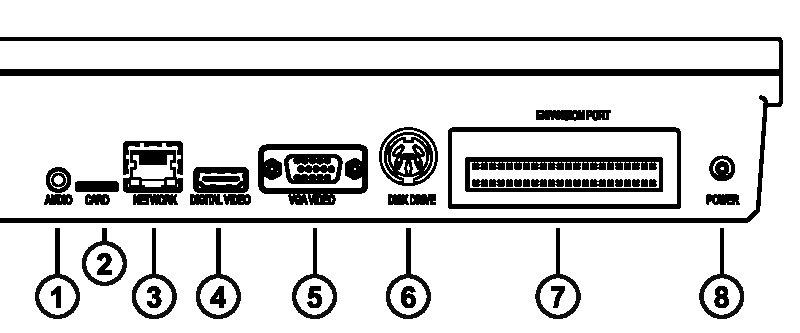
\includegraphics[width=\linewidth]{images/illustrations/mega65-rear.pdf}

\begin{center}
\setlength{\def\arraystretch{1.5}\tabcolsep}{6pt}
\begin{longtable}{ c | l}

	1	& 	3.5mm Audio Mini-Jack \\
	2	& 	SD Card Slot\\
	3	& 	Network LAN Port \\
	4	& 	Digital Video Connector \\
	5	& 	VGA Video Connector \\
	6	& 	External Floppy Disk Drive Connector \\
	7	& 	Cartridge Expansion Port \\
	8	& 	DC Power-In Socket \\

\end{longtable}
\end{center}

\newpage

\section{Side Connections}

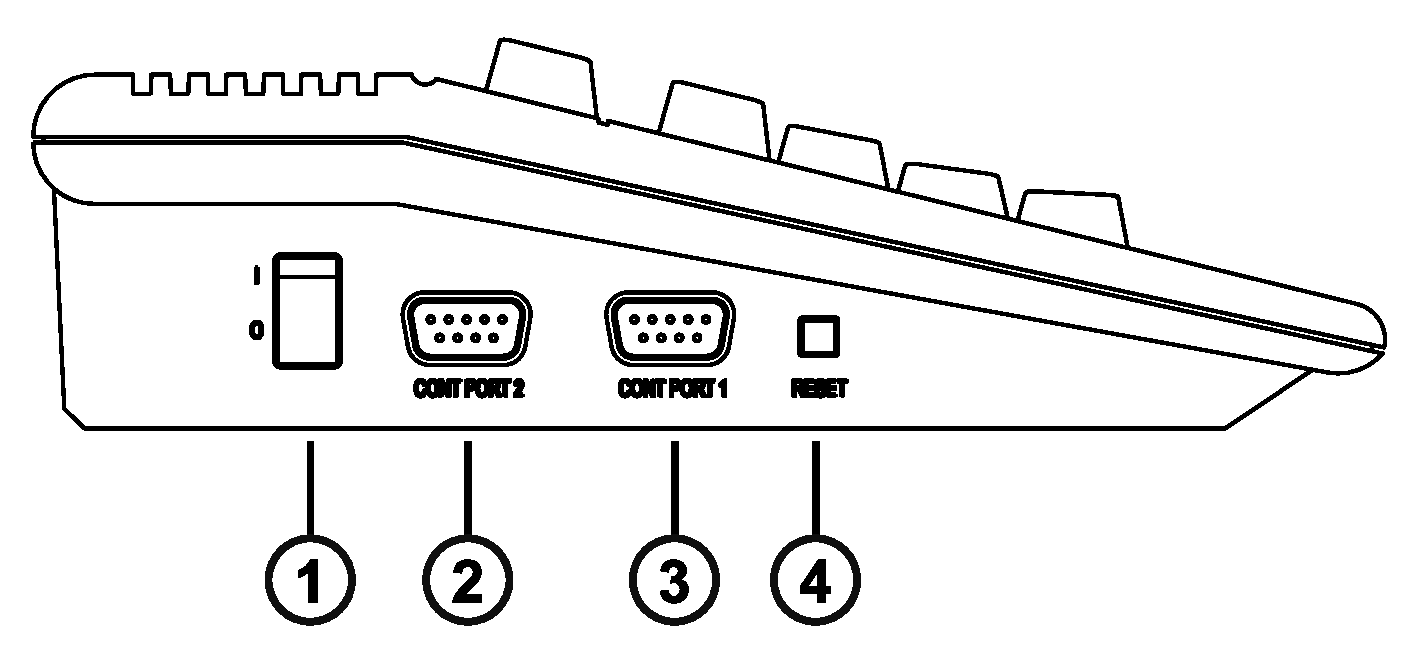
\includegraphics[width=\linewidth]{images/illustrations/mega65-side.pdf}

\begin{center}
\setlength{\def\arraystretch{1.5}\tabcolsep}{6pt}
\begin{longtable}{ c | l}

	1	& 	Power Switch \\
	2	& 	Controller Port 2 \\
	3	& 	Controller Port 1 \\
	4	& 	Reset Button \\

\end{longtable}
\end{center}

Various peripherals can be connected to Controller Ports 1 and 2 such as joysticks or paddles.

\newpage

\section{Installation}

\subsection{Connecting your MEGA65 to a screen and peripherals}

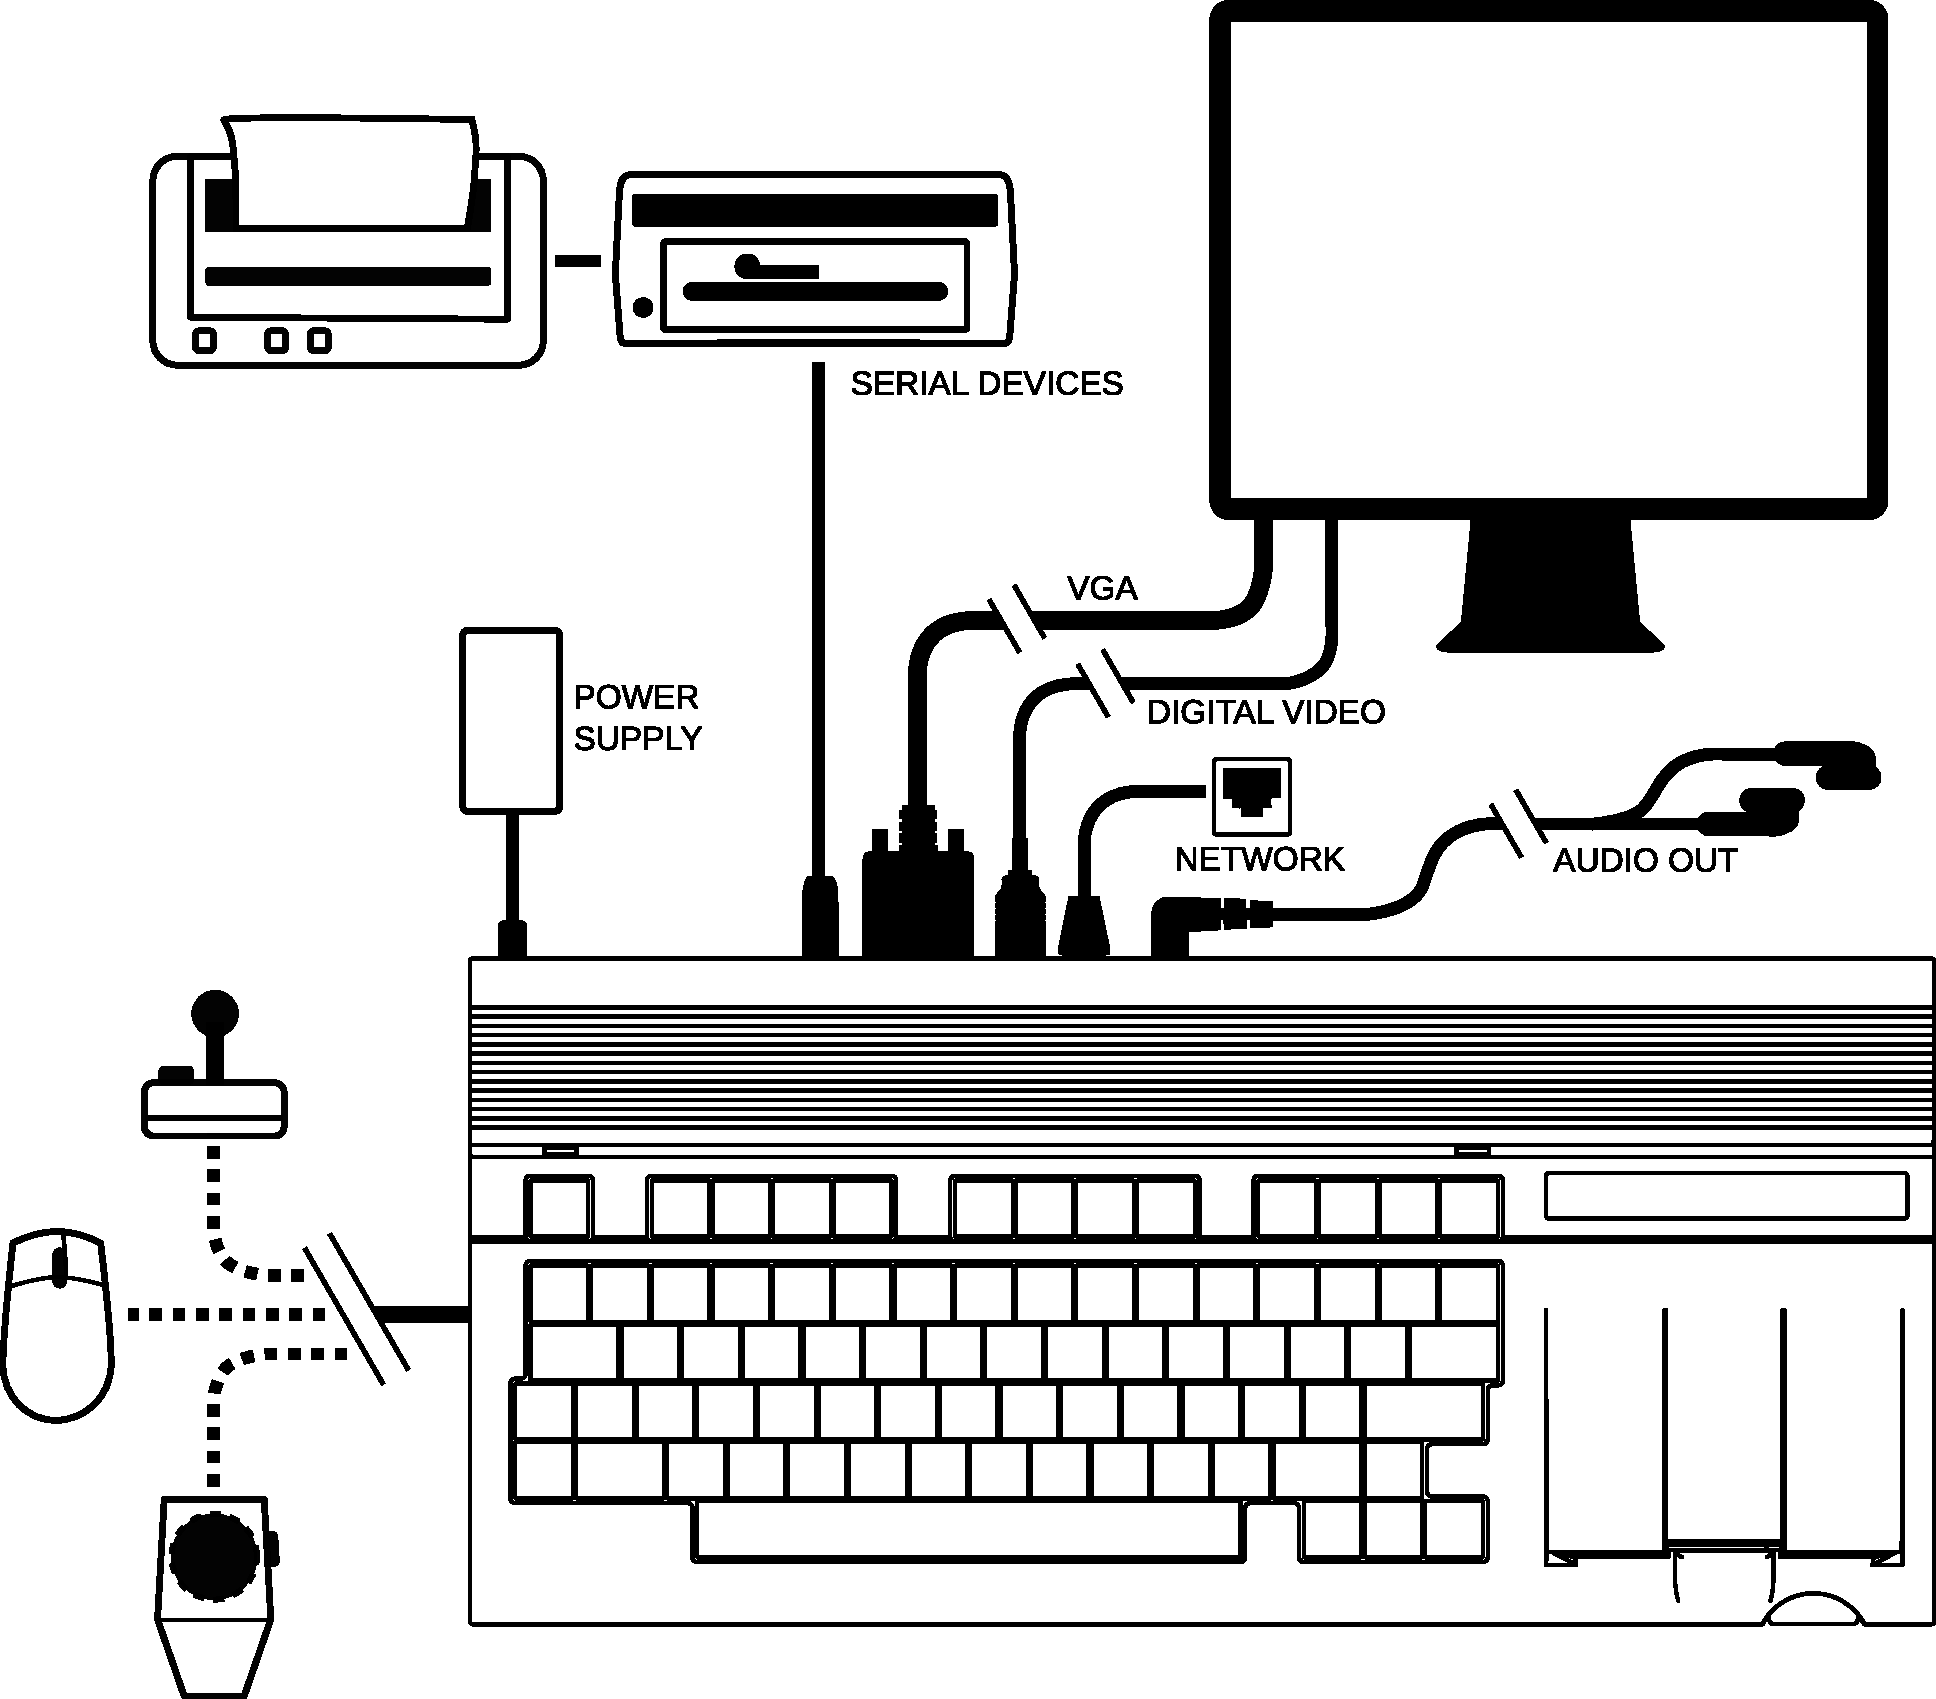
\includegraphics[width=\linewidth]{images/illustrations/mega65-top.pdf}

\newpage

\begin{enumerate}
	\item Connect the power supply to the Power Supply socket of the MEGA65.
	\item If you have a VGA monitor and a VGA cable, connect one end to the VGA port of the MEGA65 and the other end into your VGA monitor.
	\item If you have a TV or monitor with a compatible Digital Video connector, connect one end of your cable to the Digital Video port of the MEGA65, and the other into the Digital Video port of your monitor. If you own a monitor with a DVI socket, you can use a DVI to Digital Video adaptor.
\end{enumerate}

\section{Optional Connections}

\begin{enumerate}
	\item The MEGA65 includes an internal 3.5" floppy disk drive. You can also connect older Commodore{\textregistered} IEC serial floppy drives to the MEGA65, such as the Commodore{\textregistered} 1541, 1571 or 1581. To use these drives, connect one end of your IEC cable to the Commodore{\textregistered} floppy disk drive and the other end to the Disk Drive socket of the MEGA65. You can also connect SD2IEC devices and Pi1541's. It is possible to daisy-chain additional floppy disk drives or Commodore{\textregistered} compatible printers.
	\item You can connect your MEGA65 to an Ethernet network using a standard Ethernet cable.
	\item For enjoying audio from your MEGA65, you can connect a 3.5mm stereo mini-jack cable to an audio amplifier or speaker system. If your system has RCA connectors you will need a 3.5mm mini-jack to twin RCA adaptor cable. The MEGA65 also has a built in amplifier to allow the use of headphones.
	\item A Secure Digital Card or SD Card (SDHC and SDXC) can be inserted into the SD Card slot at the rear of the MEGA65 as a drive.
\end{enumerate}


\section{Operation}

\subsection{Using the MEGA65}

\begin{enumerate}
	\item Turn on the MEGA65 by using the switch on the left hand side.
	\item After a moment, the following will be displayed on your TV or monitor:
\end{enumerate}

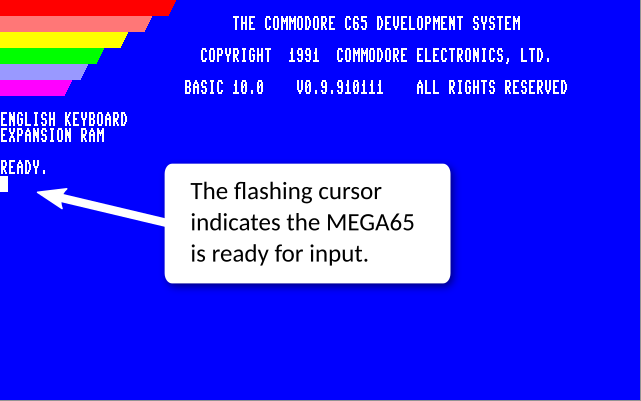
\includegraphics[width=\linewidth]{images/introduction-screen/switched-on.png}

\subsection{THE CURSOR}

The flashing square underneath the READY prompt is called the cursor. The cursor indicates that the computer is ready to accept input. Pressing keys on the keyboard will print that character onto the screen. The character will be printed at the current cursor position, and the cursor will advance to the next position.

You can type commands, for example: telling the computer to load a program. You can even start entering program code.

\chapter{Getting Started}
\phantomsection
\section{Keyboard}
\label{cha:getting-started}

Now that everything is connected, it's time to get familiar with the MEGA65 keyboard.

You may notice that the keyboard is a little different from the keyboards used on computers today. While most keys will be in familiar positions, there are some specialised keys, and some with special graphic symbols marked on the front.

Here's a brief description of how some of these special keys function.

\subsection{Command Keys}

The Command Keys are: \specialkey{RETURN}, \specialkey{SHIFT}, \specialkey{Ctrl}, \megasymbolkey and \widekey{RESTORE}.

\subsubsection{RETURN}

Pressing the \specialkey{RETURN} key enters the information you have typed into the MEGA65's memory. The computer will either act on a command, store some information, or display an error message if you made a mistake.

\subsubsection{SHIFT}

The two \specialkey{SHIFT} keys are located on the left and the right. They work very much like the Shift key on a regular keyboard, however they also perform some special functions as well.

In upper case mode, holding down \specialkey{SHIFT} and pressing any key with a graphic symbol on the front produces the right-hand symbol on that key. For example, \specialkey{SHIFT} and \megakey{J} prints the \graphicsymbol{J} character.

In lower case mode, pressing \specialkey{SHIFT} and a letter key prints the upper case letter on that key.

Finally, holding down the \specialkey{SHIFT} key and pressing a Function key accesses the function shown on the front of that key. For example: \specialkey{SHIFT} and \megakey{F1} activates \textbf{F2}.


\subsubsection{SHIFT LOCK}

In addition to the Shift key is \specialkey{SHIFT\\LOCK}. Press this key to lock down the Shift function. Now any key you press while the Shift Lock key is illuminated prints the character to the screen as if you were holding down \specialkey{SHIFT}. This includes special graphic characters.

\subsubsection{CTRL}

\specialkey{CTRL} is the Control key. Holding down \specialkey{CTRL} and pressing another key allows you to perform Control Functions. For example, holding down \specialkey{CTRL} and one of the number keys allows you to change text colours. The colour that is printed at the top row on the front of the number key will be used.

There are some examples of this in \bookvref{sec:screen-editor}, and all the Control Functions are listed in \bookvref{appendix:controlcodes}.

If a program is being LISTed to the screen, holding down \specialkey{CTRL} slows down the display of each line.

Holding \specialkey{CTRL} and pressing \megakey{*} enters the Matrix Mode Debugger.

\subsubsection{RUN/STOP}

Normally, pressing the \specialkey{RUN\\STOP} key stops execution of a program. Holding \specialkey{SHIFT} while pressing \specialkey{RUN\\STOP} loads the first program from disk.

Programs are able to disable the \specialkey{RUN STOP} key.

You can boot your MEGA65 into the machine code monitor by holding down \specialkey{RUN\\STOP} and pressing reset on the left-hand side.

\subsubsection{RESTORE}

The computer screen can be restored to a clean state without clearing the memory by holding down the \specialkey{RUN\\STOP} key and pressing \widekey{RESTORE}. This combination also resets operating system vectors and re-initialises the screen editor, which makes it a handy combination if the computer has become a little confused.

Programs are able to disable this key combination.

You can also enter the Freeze Menu by holding down \widekey{RESTORE} for more than one second. You can then access the machine code monitor via the Freeze menu.

\newpage

\subsubsection{THE CURSOR KEYS}

At the bottom right-hand side of the keyboard are the cursor keys. These four directional keys allow you move the cursor to any position for on-screen editing.

The cursor moves in the direction indicated on the keys: \megakey{$\leftarrow$} \megakey{$\uparrow$} \megakey{$\rightarrow$} \megakey{$\downarrow$}

However, it is also possible to move the cursor up using \specialkey{SHIFT} and \megakey{$\downarrow$}. In the same way you can move the cursor left using \specialkey{SHIFT} and \megakey{$\rightarrow$}.

You don't have to keep pressing a cursor key over and over. If you need to move the cursor a long way, you can keep the key pressed down. When you are finished, simply release the key.

\subsubsection{INSerT/DELete}

This is the INSERT / DELETE key. When pressing \specialkey{INST\\DEL}, the character to the left is deleted, and all characters to the right are shifted one position to the left.

To insert a character, hold the \specialkey{SHIFT} key and press \specialkey{INST\\DEL}. All the characters to the right of the cursor are shifted to the right. This allows you to type a letter, number or any other character into the newly inserted space.


\subsubsection{CLeaR/HOME}

Pressing the \specialkey{CLR\\HOME} key returns the cursor into the top left-most position of the screen.

Holding down \specialkey{SHIFT} and pressing \specialkey{CLR\\HOME} clears the entire screen and places the cursor into the top left-most position of the screen.

\subsubsection{MEGA KEY}

The \megasymbolkey key or the MEGA key provides a number of different functions and can be used to launch special utilities.

Holding the \specialkey{SHIFT} key and pressing \megasymbolkey switches between lower and upper-case character modes.

Holding \megasymbolkey and pressing any key with graphic symbols on the front prints the left-most graphic symbol to the screen.

Holding \megasymbolkey and pressing any key that shows a single graphic symbol on the front prints that graphic symbol to the screen.

Holding \megasymbolkey and pressing a number key switches to one of the colours in the second range. The colour that is printed at the bottom row on the front of the number key will be used.

Holding \megasymbolkey and pressing \specialkey{TAB} enters the Matrix Mode Debugger.

Switching on the MEGA65 or pressing the reset button on the left-hand side while holding down \megasymbolkey switches the MEGA65 into C64 mode.

\subsubsection{NO SCROLL}
If a program is being LISTed to the screen, pressing \specialkey{NO\\SCROLL} freezes the screen output. This feature is not available in C64 mode.


\subsection{Function Keys}

There are seven Function keys available for use by software applications, \megakey{F1} \megakey{F3} \megakey{F5} \megakey{F7} \megakey{F9} \megakey{F11} and \megakey{F13} can be used to perform functions with a single press.

Hold \specialkey{SHIFT} to access \megakey{F2} through to \megakey{F14} as shown on the front of each Function key.

Only Function keys \megakey{F1} to \megakey{F8} are available in C64 mode.

\subsubsection{HELP}

The \specialkey{HELP} key can be used by software and acts as an \megakey{F15} / \megakey{F16} key.

\subsubsection{ALT}

Holding \specialkey{ALT} down while pressing other keys can be used by software to perform functions. Not available in C64 mode.

Holding \specialkey{ALT} down while switching the MEGA65 on activates the Utility Menu. You can format an SD card, or enter the MEGA65 Configuration Utility to select the default video mode and other settings, or test your keyboard.

\subsubsection{CAPS LOCK}

The \specialkey{CAPS\\LOCK} works like \specialkey{SHIFT\\LOCK} in C65 and MEGA65 modes, but only modifies the alphabet keys.
Also, holding the \specialkey{CAPS\\LOCK} key down forces the processor to run at the maximum speed. This can be used, for example,
to speed up loading from the internal disk drive or SD card, or to greatly speed up the de-packing process after a program is run.
This can reduce the loading and de-packing time from many seconds to as little as a fraction of a second.

\section{The Screen Editor}
\label{sec:screen-editor}

When you switch on your MEGA65 or reset it, the following screen will appear:

\begin{center}
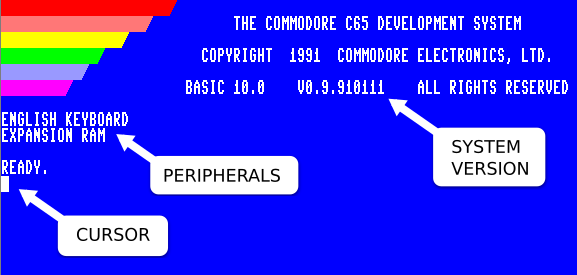
\includegraphics[width={10cm}]{images/introduction-screen/layout.png}
\end{center}

The colour bars in the top left-hand side of the screen can be used
as a guide to help calibrate the colours of your display.
The screen also displays the name of the system,
the copyright notice, and the ROM version.
The displayed date and time are taken from the internal RTC
(Real-Time Clock), which can be set in the Configure Menu.

Finally, you will see the \screentext{READY} prompt and the flashing cursor.

You can begin typing keys on the keyboard and the characters will be
printed at the cursor position. The cursor itself will advance after
each key press.

You can also produce reverse text or colour bars by holding down \specialkey{CTRL} and pressing \megakey{9}, or \megakey{R}. This enters reverse text mode. When this is enabled, you can press and hold the \megakey{Space} bar. While doing so, a white bar will be drawn across the screen.
\index{Keyboard!CTRL}
You can even change the current colour by holding \specialkey{CTRL} down and pressing a number key (from \megakey{1} to \megakey{8}). For example, if you press and hold \specialkey{CTRL} down and press \megakey{1}, the colour will change to black. Now, when you hold down the \megakey{Space} bar, a black bar will be drawn. If you continue to change the colour and press the \megakey{Space} bar, you will get an effect similar to the image below:


\begin{center}
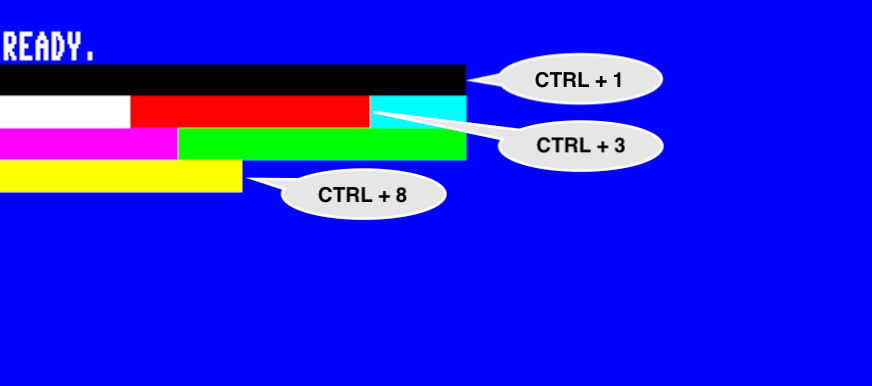
\includegraphics[width={10cm}]{images/introduction-screen/colour-bars.png}
\end{center}


\index{Keyboard!MEGA Key}
You can disable reverse text mode by holding \specialkey{CTRL} and pressing \megakey{0}.

By pressing any key, characters will be printed to the screen in the chosen colour.

A further eight colours can be selected by holding down \megasymbolkey and pressing a key from \megakey{1} to \megakey{8}.
The colour that is printed at the bottom row on the front of the number key will be used. For example, if you held
\megasymbolkey down while pressing \megakey{4}, dark gray will be used. For even more colours, see \bookvref{appendix:escape-colours}.

\needspace{4cm}
You can create fun pictures just by using these colours and letters.  Here's an example of what a year four student drew:

\begin{center}
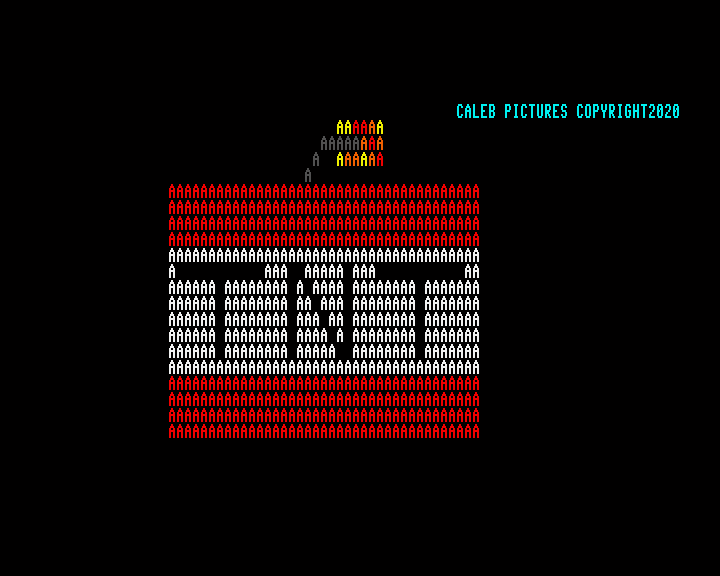
\includegraphics[width={6cm}]{images/caleb-PETSCII-TNT-final}
\end{center}

What will you draw?

\needspace{2cm}
\textbf{Functions}

Functions using \specialkey{CTRL} are called \textbf{Control Codes}.
Functions using \megasymbolkey are called \textbf{Mega Codes}. There are also functions that are called by using \specialkey{SHIFT}, which
are called \textbf{Shifted Codes}.

Lastly, \specialkey{ESC} enables the use of \textbf{Escape Sequences}.

You can read about all of these functions in detail in \bookvref{appendix:controlcodes}, but some are shown in this section.


\needspace{2cm}
\textbf{ESC Sequences}
\index{Keyboard!Escape Sequences}
Escape sequences are performed a little differently than a Control function or a Shift function. Instead of holding the modifier key down, an Escape sequence is performed by pressing \specialkey{ESC} and releasing it, followed by pressing the desired key code.

For example: to switch between 40/80 column mode, press and release \specialkey{ESC}, then press \megakey{X}.

There are more modes available. You can create flashing text by holding \specialkey{CTRL} down and pressing \megakey{O}. Any characters you type in will flash. Turn flash mode off by pressing \specialkey{ESC},  then \megakey{O}.



\section{Editor Functionality}


The MEGA65 screen can allow you to do advanced tabbing, and quickly move around the screen in many ways to help you to be more productive.

For example, press \specialkey{CLR HOME} to go to the home position on the screen. Hold \specialkey{CTRL} down and press \megakey{W} several times. This is the \textbf{Word Advance function}, which jumps your cursor to the next word, or printable character.

You can set custom tab positions on the screen for your convenience. Press \specialkey{CLR HOME} and then \megakey{$\rightarrow$} to the fourth column. Hold down \specialkey{CTRL} and press \megakey{X} to set a tab. Move another 16 positions to the right again, and press \specialkey{CTRL} and \megakey{X} again to set a second tab.

Press \specialkey{CLR HOME} to go back to the home position. Hold \specialkey{CTRL} down and press \megakey{I}. This is the \textbf{Forward Tab function}. Your cursor will tab to the fourth position. Press \specialkey{CTRL} and \megakey{I} again. Your cursor will move to position 8. Why do you ask? By default, every 8th position is already set as a tabbed position. So the 4th and 20th positions have been added to the existing tab positions. You can continue to press \specialkey{CTRL} and \megakey{I} to advance to the 16th and 20th positions.

To find the complete set of Control codes, see \bookvref{appendix:controlcodes}.

\textbf{Creating a Window}
\index{Keyboard!Escape Sequences}

You can set a window on the MEGA65 working screen. Move your cursor to the beginning of the "BASIC 65" text. Press \specialkey{ESC}, then press \megakey{T}. Move the cursor 10 lines down and 15 to the right.

Press \specialkey{ESC}, then \megakey{B}. Anything you type will be contained within this window.

For example, if you were to type \screentext{LIST} to list out a program, the listing will be confined to the window region you have specified:

\begin{center}
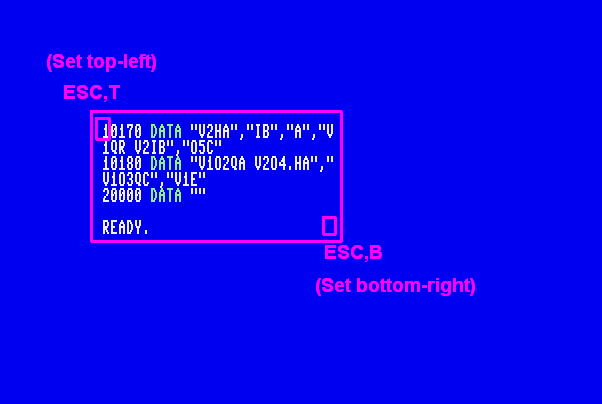
\includegraphics[width={7cm}]{images/set-window.png}
\end{center}

To escape from the window back to the full screen, press \specialkey{CLR HOME} twice.


\textbf{Extras}

Below are some extra, useful things you can do whilst in the screen editor:

  To enter the \textbf{Freeze Menu}, long press on \widekey{RESTORE}, then press \megakey{J} to switch joystick ports without 
having to physically swap the joystick to the other port. You can read more about the Freeze Menu, and what else it can do
on page \pageref{sec:freezer}.

\index{POKE}
  To enter \textbf{Fast mode} (40.5MHz), either type \screentext{SPEED} (preferred way), or \screentext{POKE 0,65} or enter the Freeze Menu and switch the CPU frequency with \megakey{F}.

  Return back to \textbf{Slow mode} (1MHz) by either typing \screentext{SPEED 1} (preferred way), or \screentext{POKE 0,64} or enter the Freeze Menu and switch the CPU frequency with \megakey{F}.

  \megasymbolkey + \specialkey{SHIFT} switches between uppercase and lowercase text for the entire display.


\part{FIRST STEPS IN CODING}

\chapter{How Computers Work}

Did you know that many computer experts and programmers learned how to
use computers when they were still small children?
Home computers only became common in the early 1980s. They were so new,
that people would often write programs to do
what they wanted to do, because no software existed to do the job for them.

It was also quite common for people working in all
sorts of office jobs to learn how to program the computers they used for
their jobs.  For example, the people processing payroll
for a company would often learn how to program the computer to calculate
the everyone's pay!

Things have changed a lot since then, though.
Now most people choose existing programs or apps to do what they need,
and think that programming is a specialised skill that only some people
have the ability to learn.
But this isn't true.  Of course, like every other field of pursuit
everyone will be better at some things than others,
whether it be sports, knitting, maths or writing. But almost
everyone is able to learn enough to help them in their life.

We created the MEGA65, because we believe that YOU can learn to
program, so that computers can be more useful to you, and as with
learning any new skill, that you can have the satisfaction and enjoyment
and new adventures that this brings!


\phantomsection
\section{Computers are stupid. Really stupid}

How can this be so? Computers are able to do so many different things, often thousands of times faster than a person can.
So how can we say that computers are stupid?  The answer is that no computer can do anything that it hasn't been instructed
by a person to do.  Even the latest Artificial Intelligence systems were instructed how to learn (or how to learn, how to learn).
To understand why this is so, it is helpful to understand how computers really work.

\subsection{Making an Egg Cup Computer}

The heart of a computer is its Central Processing Unit, or CPU for short.  Many modern computers have more than one CPU, but let's keep
things simple to begin with.  The CPU has a set of simple instructions that it understands, like, ``get the thing from cup \#21,'' ``put this thing into cup \#403,'' ``add these things together,'' or ``do the following instruction, but only if the thing in cup \#712 is the number 3.''

But what do we mean with all of these ``things'' and ``cups''? Let's start by thinking about how we could pretend to be a computer using
just an empty egg carton, some small pieces of paper and a pencil or pen.  Start by writing numbers, beginning with one, in each of the
little egg cups in the egg carton.  Then write the number zero on a little scrap of paper and put it in the first cup.  Do the same for the other cups. You should now have an egg carton with numbered cups, and with every cup having a scrap of paper with the number zero written on it. Now we just need to decide on a few simple rules that will explain how our egg-cup computer will work:

\begin{itemize}
  \item First, each cup is allowed to hold exactly one thing at a time. Never more. Never less.  This so that when we ask the question ``what is in box such-and-such,'' that there is a single clear answer. It's also how computer memory works: Each piece of memory can hold only one thing at a time.

  \item Second, we need a way for the computer to know what to do next. On most computers this is called the Program Counter, or PC, for short (not to be confused with PC when people are talking about a Personal Computer).  The PC is just the number of the next of the next memory location (or in our case, egg-cup), that the computer will examine, when deciding what to do next.  You might like to have another piece of paper that you can use to write the PC number on as you go along.

  \item Third, we need to have a list of things that the egg-cup computer will do, based on what number is in the egg-cup indicated by the 
    PC.
\end{itemize}

So let's come up with the set of things that the computer can do, based on the number in the egg-cup indicated by the PC.  We'll keep things simple with just the following:

\begin{center}
  \begin{longtable}{|R{2.2cm}|p{8cm}|}

    \hline
        {\textbf{Number in the egg-cup}} & {\textbf{Action}} \\ \hhline{|=|=|}
        0 & {i) Add one to the PC, and do nothing else.} \\ \hline
        1 & {i) Add one to the PC. \hfill\break ii) Set the PC to be the number stored in that egg-cup.} \\ \hline
        2 & {i) Add one to the PC. \hfill\break ii) Add the number in the egg-cup indicated by the PC to the number in the egg-cup indicated by the number in the egg-cup following that. \hfill\break iii) Put the answer in the egg-cup indicated by the egg-cup following that. \hfill\break iv) Finally, add two more to the PC, to skip over the egg-cups that we made use of.}  \\ \hline
  \end{longtable}
\end{center}

Don't worry if that sounds a bit confusing for now, specially that last one -- we will go through it in detail very soon!
The best way to explain it, is to go through some examples.


\chapter{Getting Started in BASIC}
\label{cha:basic-getting-started}

It is possible to code on the MEGA65 in many languages,
however most people start with BASIC.  That makes sense,
because BASIC stands for Beginner's All-purpose Symbolic
Instruction Code: It was made for people like you to get
started with in the world of coding!

A few short words before we dive in: BASIC is a programming
language, and like spoken language it has conventions, grammar
and vocabulary.  Fortunately, it is much quicker and easier
to learn than our complex human languages. But if you pay
attention, you might notice some of these structures, and that
can help you along your path in the world of coding.

If you haven't already read Chapter \ref{cha:getting-started},
it might be a good idea to do so. This will help you be able to
more confidently interact with the MEGA65 computer.

It's also great to remember that if you really confuse the MEGA65,
you can always get back to the READY. prompt by just pressing the
reset button on the left-hand side of the keyboard, or if that
doesn't help, then by turning it off
and on again using the power switch on the left-hand side of the keyboard.
You don't have to worry about shutting the computer
down properly or any of that nonsense.  The only thing to remember
is that if you had any unsaved work, it will be lost when you turn
the computer off and on again or press the reset button.

Finally, if you don't understand all of the descriptions and information
with an example -- don't worry! We have provided as much information
as we can, so that it is there in case you have questions, encounter problems are are
just curious to discover more.  Feel free to skip ahead to the examples
and try thing out, and then you can go back and re-read it when you are motivated
to find something out, or help you work though a problem.  And if you don't find
the answer to your problem, send us a message!  There are support forums for the
MEGA65 at \url{https://mega65.net}, and you can
report problems with this guide at:

\url{https://github.com/mega65/mega65-user-guide}

We hope you have as much fun learning to programme the MEGA65 as
we have had making it!

\section{Your first BASIC programmes}

The MEGA65 was designed to be programmed! When you turn it on,
it takes a couple of seconds to get its house in order, and then
it quickly shows you a ``READY.'' prompt and flashing block called
the cursor.  When the cursor is blinking, it tells you that the
computer is waiting for input.  The ``READY.'' message tells you
that the BASIC programming language is running and ready for you to
start programming.  You don't even need to load any programmes --
you can just get started.

Try typing the following into the computer and see what happens:

\begin{screenoutput}
HELLO COMPUTER
\end{screenoutput}

To do this, just type the letters as you see them above.  The computer
will already be in upper-case mode, so you don't need to hold the \specialkey{SHIFT}
or \specialkey{CAPS\\LOCK} key down.  When you have typed ``HELLO COMPUTER'' press
  the \specialkey{RETURN} key.  This tells the computer you want it to accept the
  line of input you have typed.  When you do this, you should see a message something
  like the following:

\screenshotwrap{images/syntax-error.png}
  
  If you saw a \screentextwide{SYNTAX ERROR} message something like that one, then congratulations:
  You have succeeded in communicating with the computer!\index{Errors!Syntax}\index{SYNTAX ERROR}
  Error messages sound much nastier than they are.  The MEGA65 uses them, especially
  the syntax error to tell you when it is having trouble understanding what you have
  typed, or what you have put in a programme.  They are nothing to be afraid of, and
  experienced programmers get them all the time.

  In this case, the computer was confused because it doesn't understand the word
  ``hello'' or the word ``computer''.  That is, it didn't know what you wanted it to
  do.  In this regard, computers are quite stupid. They know only a few words, and
  aren't particularly imaginative about how they interpret them.

  So let's try that again in a way that the computer will understand.  Try typing
  the following in.  You can just type it right away. It doesn't matter that the
  syntax error message can still be seen on the screen.  The compute has already
  forgotten about that by the time it told you \screentextwide{READY.} again.

\begin{screenoutput}
PRINT "HELLO COMPUTER"
\end{screenoutput}

Again, make sure you don't use shift or shift-lock while typing it in.  The symbols around
the words \screentextwide{HELLO COMPUTER} are double-quotes.  If you are used to an Australian or American
keyboard, you might discover that they double-quote key is in a rather different place to
where you are used to:  Double-quotes can be typed on the MEGA65 by holding down the
\specialkey{SHIFT} key, and then pressing 2.  Don't forget to press the \specialkey{RETURN}
key when you are done, so that the computer knows you want it to do something with your input.

If you make a mistake while typing, you can use the \specialkey{INST\\DEL} to rub out the mistake
and fix it up.  You can also use the cursor keys to move back and forth on the line while
you edit the line you are typing, but there is a bit of a trick if you have already typed
a double-quote: If you try to use the cursor keys, it will print a funny reversed symbol
instead of moving the cursor.  This is because the computer thinks you want to record
moving the cursor in the text itself, which can be really useful and fun, and which you can
read more about in Chapter \ref{cha:getting-started}. But for now, if you
make a mistake just press the \specialkey{RETURN} key and type the messed up line again.
Hopefully now you will see something like the following:

\screenshotwrap{images/print-hello-computer.png}

  This time no new \screentextwide{SYNTAX ERROR} message should appear. But if some kind
  of error message has appeared, just try typing in the command again, after
  taking a close look to work out where the mistake might be.

  Instead of an error, we should see \screentextwide{HELLO COMPUTER} repeated underneath
  the line you typed in.  The reason this happened is that the computer
  does understand the word \screentextwide{PRINT}.  It knows that whatever comes after
  the word \screentextwide{PRINT} should be printed to the screen.  We had to put \screentextwide{HELLO
  COMPUTER} inside double-quotes to tell the compute that we want it to be
  printed literally.

  If we hadn't put the double-quotes in, the computer would have thought
  that \screentextwide{HELLO COMPUTER} was the name of a stored piece of information.
  But because we haven't stored any piece of information in such a place,
  the computer will have zero there, so the computer will print the number
  zero, like this. If the computer prints zero or some other number when
  you expected a message of some sort, this can be the reason.

  You can try it, if you like, and you should see something like the following:

  \screenshotwrap{images/print-hello-computer-no-quotes.png}

  In the above examples we typed commands in directly, and the computer executed
  them immediately after you pressed the \specialkey{RETURN} key.  This is why
  typing commands in this way is often called {\em direct mode} or {\em immediate mode}.
  
  But we can also tell the computer to remember a list of commands to execute one
  after the other.   This is done using the rather unimaginatively named {\em non-direct mode}.
  To use non-direct mode, we just put a number between 0 and 63999 at the start of
  the command.  The computer will then remember that command.  Unlike when we executed
  a direct-mode command, the computer doesn't print \screentextwide{READY.} again. Instead the cursor
  just reappears on the next line, ready for us to type in more commands.

  Let's try that out with a simple little programme.  Type in the following three lines of
  input:

\begin{screenoutput}
1 FOR I = 1 TO 10 STEP 1
2 PRINT I
3 NEXT I
\end{screenoutput}
\index{FOR}
\index{BASIC 10 Commands!FOR}

When you have done this, the screen should show something like this:

\screenshotwrap{images/first-steps-for-loop-programme-1.png}

If it doesn't you
can try again. Don't forget, if you feel that the computer is getting all muddled up,
you can just press the reset button or flip the power switch off and on on the left side of the
computer to reboot it. This only takes a couple of seconds, and doesn't hurt the MEGA65
in anyway.

We have told the computer to remember three commands, that is, \screentextwide{FOR I = 1 TO 10 STEP 1},
\screentextwide{PRINT I}
and \screentextwide{NEXT I}.  We have also told the computer which order we would like to run them in: The
computer will start with the command with the lowest number, and execute each command that
has the next higher number in turn, until it reaches the end of the list.  So it's a bit like
a reminder list for the computer. This is what we call a programme, a bit like the programme at
a concert or the theatre, it tells us what is coming up, and in what order.
So let's tell the computer to execute this programme.

But first, let's try to guess what will happen.  Let's start with the middle command, \screentextwide{PRINT I}.
We've seen the \screentextwide{PRINT} command, and we know it tells the computer to print things to the screen.
The thing it will try to print is \screentextwide{I}.  Just like before, because there are no double-quotes
around the \screentextwide{I}, it will try to print a piece of stored information.  The piece of information
it will try to print will be the piece associated with the thing \screentextwide{I}.

When we give a piece of
information like this a name, we call it a {\em variable}\index{variable}.  They are called
variables because they can vary.  That is, we can replace the piece of information associated
with the variable called I with another piece of information.  The old piece will be forgotten
as a result.  So if we gave a command like \screentextwide{LET I = 3}, this would replace whatever was stored
in the variable called \screentextwide{I} with the number 3.

Back to our programme, we now know that the 2\textsuperrscript{nd} command will try to print the piece of information
stored in the variable \screentextwide{I}.  So lets look at the first command: \screentextwide{FOR I = 1 TO 10 STEP 1}.  Although
we haven't seen the \screentextwide{FOR} command before, we can take a bit of a guess at how it works. It looks like
it is going to put something into the variable \screentextwide{I}.  That something seems to have something to do
with the range of number 1 through 10, and a step or interval of 1.  What do you think it will do?

If you guessed
that it will put the values 1, 2, 3, 4, 5, 6, 7, 8, 9 and then 10 into the variable \screentextwide{I}, then you
can give yourself a pat on the back, because that's exactly what it does.  It also helps us to
understand the 3\textsuperscript{rd} command, \screentextwide{NEXT I}: That command tells the computer to put the next value into
the variable \screentextwide{I}.  And here is a little bit of magic: When the computer does that, it goes back
up the list of commands, and continues again from the command after the \screentextwide{FOR} command.

So lets pull that together: When the computer executes the first command, it discovers that it has
to put 10 different values into the variable \screentextwide{I}. It starts by putting the first value in there, which
in this case will be the number 1.
The computer then continues to the second command, which tells the computer to print the piece of
information that is currently stored in the variable called \screentextwide{I}. That will be the number 1, since
that was the last thing the computer was told to put there.  Then the computer proceeds to the
third command, which tells it that it is time to put the next value into the variable \screentextwide{I}.  So the
computer will throw away the number 1 that is currently in the variable \screentextwide{I}, and put the number 2 in
there, since that is the next number in the list.  It will then continue from the 2\textsuperscript{nd} command,
which will cause the computer to print out the contents of the variable \screentextwide{I} again.  Except that this
time \screentextwide{I} has had the number 2 stored in it most recently, so the computer will print the number 2.
This process will repeat, until the computer has printed all ten values that the \screentextwide{FOR} command
indicated it to do.   

To see this in action, we need to tell the computer to execute the programme of commands we typed in.
We do this by using the \screentextwide{RUN} command. Because we want it to run the programme immediately, we
should use immediate mode (remember, this is another name for direct mode).
So just type in the word \screentextwide{RUN} and press the \specialkey{RETURN} key.  You should then see a display
that looks something like the following:

\screenshotwrap{images/first-steps-for-loop-programme-1-running.png}

  You might notice a couple of things here:

  First, the computer has told us it is \screentextwide{READY.} again
  as soon as it finished running the programme. This just makes it easier for us to know when we
  can start giving commands to the computer again.

  Second, when the computer got to the bottom of the screen
  it automatically scrolled the display up to make space.  This is quite normal.  What is important
  to remember, is that the computer forgets everything that scrolls off the top.  The only exception
  is if you have told the computer to remember a command by putting a number in front of it.  So
  our programme is quite safe for now. We can see that this is the case by typing the \screentextwide{RUN} command a
  couple more times: The programme listing will have scrolled off the top of the screen, but we can
  still RUN the programme, because the computer has remembered it.  Give it a try!
  Did it work?

  If you wish to see the programme of remembered commands, you can use the \screentextwide{LIST}\index{LIST}\index{BASIC 10 Commands!LIST}
  command.  This commands causes the computer to display the remembered programme of commands to the screen, like in the display here.
  If you would like to replace any of the commands in the programme, you can type a new line that has the same number as the one you
  wish to change. 

\screenshotwrap{images/first-steps-for-loop-programme-1-listing.png}

  For example, to print the results all on one line, we could modify the second line of the programme to \screentextwide{PRINT I;} by
  typing the following line of input and pressing the \specialkey{RETURN} key:


  
\begin{screenoutput}
2 PRINT I;
\end{screenoutput}

\index{PRINT}
\index{BASIC 10 Commands!PRINT}
%\end{tcolorbox}

You can make sure that the change has been remembered by running the \screentextwide{LIST} command again, as we can see here.
You can then use the \screentextwide{RUN} command to run the modified programme.

\screenshotwrap{images/first-steps-for-loop-programme-1-modified.png}

It is quite easy to modify your programmes in this way.  As you become more comfortable with the process, there are two
additional helpful tricks:

First, you can give the \screentextwide{LIST} command the number of a command, or line as they are referred to, and it will display only
that line of the programme.  Alternatively, you can give a range separated by a minus sign to display only a section of the programme,
e.g., \screentextwide{LIST 1 - 2} to list the first two lines of our programme.

Second, you can use the cursor keys to move the cursor to a line which has already been remembered and is displayed on the screen. If you
modify what you see on the screen, and then press the \specialkey{RETURN} key while the cursor is on that line, the BASIC interpreter will
read in the modified line and replace the old version of it.  It is important to note that if you modify multiple lines of the programme
at the same time, you must press the \specialkey{RETURN} key on each line that has been modified. It is good practice to check that the
programme has been correctly modified. Use the \specialkey{LIST}\index{LIST}\index{BASIC 10 Commands!LIST} command again to achieve this.
  
  
  \subsubsection{Exercises to try}

  {\bf 1. Can you make it count to a higher or lower number?}

  At the moment it counts from 1 to 10.  Can you change it to count to 20 instead?  Or to count from 3 to 17?
  Or how about from 14.5 to 21.5? What do you think you would need to reverse the order in which it counts?

  {\em Clue:} You will need to modify the \screentextwide{FOR} command.  

  {\bf 2. Can you change the counting step?}

  At the moment it counts by ones, i.e., each number is one more than the last.  Can you change it to count by twos
  instead? Or by halves, so that it counts 1, 1.5, 2, 2.5, 3, \ellipsis?
  
  {\em Clue:} You will need to modify the \screentextwide{STEP} clause of the \screentextwide{FOR} command.\index{STEP}\index{BASIC10 Commands!STEP}
  
  
  {\bf 3. Can you make it print out one of the times tables?}
  
  At the moment it prints the answers to the 1 times tables, because it counts by ones.
  Can you make it count by threes, and show the three times tables?
  
  {\em Clue:} You will need to modify the \screentextwide{FOR} command.
  
  {\bf 4. Can you make it print out the times tables from 1$\times$1 to 10$\times$10?}
  
  {\em Clue:} You might like to use ; on the end of \screentextwide{PRINT} statements, so that you can have
  more than one entry per line on the screen.\\
  {\em Clue:} The \screentextwide{PRINT} statement without any argument will just advance to the start of the next line.\\
  {\em Clue:} You might need to have multiple \screentextwide{FOR} loops, one inside the other.
  
\section{First steps with text and numbers}

\section{Making simple decisions}

\section{Random numbers and chance}

\include{morebasic}
\include{datainbasic}

\part{SOUND AND GRAPHICS}

%\usepackage{colortbl}
%\usepackage{adjustbox}


\newcommand{\blkb}{\cellcolor[rgb]{0,0,0}\textcolor{white} 0 }
\newcommand{\bwn}{\cellcolor[rgb]{.26,.22,0}\textcolor{white} 9 }
\newcommand{\ora}{\cellcolor[rgb]{.44,.31,.15} 8 }
\newcommand{\red}{\cellcolor[rgb]{.6,.4,.35} A }
\newcommand{\lgr}{\cellcolor[rgb]{.58,.58,.58} F }
\newcommand{\yel}{\cellcolor[rgb]{.72,.78,.44} 7 }

\newcommand{\redb}{\cellcolor[rgb]{.6,.4,.35} 1 }

\chapter{Graphics}
\label{cha:graphics}

Let's have some fun with graphics!
In this part of the book, we want to examine the MEGA65's graphics modes by walking through example code in machine language to get to know the various options of the MEGA65 in the area of graphics. First of all, it is important to know that the MEGA65 supports three different basic graphics modes:

\begin{itemize}
	\item Bitmap graphics
	\item Graphics based on character sets
	\item Bitplanes
\end{itemize}


\section*{Bitmap Graphics}

In bitmap graphics every pixel of a graphic is stored separately. The way the pixels are hold in memory varies from system to system and in most cases depends on the performance of the hardware. If memory would be unlimited, the easiest way to remember a pixel is to save its RGB-values in three separate bytes. Example: 0xFFFFFF for white would result in three values to be stored: \$FF, \$FF and \$FF. To be honest, this is too simple and not really efficient. Let’s think about another way. Why not defining a color table (or color palette) and store the RGB values once and finally only reference the color by its index in the table? This will save us a lot of memory! Let's imagine we would create a colorful 8x8 bitmap to represent an "A" on the screen. Colourful means, we want it in some brownish colors. The color table for it may look like this:

%\setlength\minrowclearance{4pt}
\begin{center}
\begin{tabular}{|m{22pt}|m{60pt}|}
\hline
	Index & Color \\
\hline
	\blkb & Black \\
	\bwn & Brown \\
	\ora & Orange \\
	\red & Light Red \\
	\lgr & Light Grey \\
	\yel & Yellow \\
\hline
\end{tabular}
\end{center}

The color values, by the way, are exact the same as the color values from the standard C64 color palette. Next we design the "A". Each pixel references a value from the color table above.


%\setlength\minrowclearance{4pt}
\begin{center}
\begin{tabular}{|m{4pt}|m{4pt}m{4pt}m{4pt}m{4pt}m{4pt}m{4pt}m{4pt}m{4pt}|}
\hline
	& 7 & 6 & 5 & 4 & 3 & 2 & 1 & 0 \\
\hline
	0 & \blkb & \blkb & \blkb & \blkb & \blkb & \blkb & \blkb & \blkb \\
	1 & \red & \lgr & \yel & \lgr & \red & \ora & \blkb & \blkb \\
	2 & \lgr & \lgr & \blkb & \blkb & \ora & \red & \blkb & \blkb \\
	3 & \yel & \yel & \blkb & \blkb & \ora & \red & \blkb & \blkb \\
	4 & \yel & \lgr & \lgr & \red & \red & \red & \blkb & \blkb \\
	5 & \lgr & \red & \blkb & \blkb & \ora & \red & \blkb & \blkb \\
	6 & \red & \red & \blkb & \blkb & \red & \red & \blkb & \blkb \\
	7 & \ora & \bwn & \blkb & \blkb & \ora & \red & \blkb & \blkb \\
\hline
\end{tabular}
\end{center}

But how much memory does this little graphic use?

If we create an one-dimensional array, we will get an array with 64 elements, because our graphic consists of 8x8 pixels = 64 color values that have to be saved. If we transfer that to the memory of the MEGA65, it means that we have 64 bytes to store in memory. However, full-screen graphics are made up of far more pixels. On the C64 and of course also on the MEGA65, 320x200 pixels are required to generate a graphic that fills the entire screen. If we transfer this to our array, we would have a total of 64,000 entries. Converted to the memory of the MEGA65, that is 64,000 bytes or nearly 64 kilobytes of data! If we now also consider that the good old C64 only had 64K of RAM available, we recognize the Drama! That's just too much data! We need strategies to reduce our bitmap data. On the C64 we had to two types of bitmap graphics and both come with its own concepts to use as less memory as possible.

\begin{itemize}
	\item Hires
	\item Multicolor (MCM)
\end{itemize}


\subsection*{Hires}

First, a bitmap is divided into blocks of 8x8 pixels each. In order to achieve the full resolution of 320x200 pixels, 40 of such blocks next to each other builds up a line. If we now build up 25 lines, we arrive at a graphic that fills the complete screen.

\begin{adjustbox}{width=\textwidth,center}
\begin{center}
\begin{footnotesize}
\begin{tabular}[h]{|C{10pt}|C{5pt}|C{5pt}|C{5pt}|C{5pt}|C{5pt}|C{5pt}|C{5pt}|C{5pt}|C{5pt}|C{5pt}|C{5pt}|C{5pt}|C{5pt}|C{5pt}|C{5pt}|C{5pt}|C{5pt}|C{5pt}|C{5pt}|C{5pt}|C{5pt}|C{5pt}|C{5pt}|C{5pt}|C{5pt}|C{5pt}|C{5pt}|C{5pt}|C{5pt}|C{5pt}|C{5pt}|C{5pt}|C{5pt}|C{5pt}|C{5pt}|C{5pt}|C{5pt}|C{5pt}|C{5pt}|C{5pt}|}
\hline
  &   &   &  &  &  &   &   &   &   & 1  & 1  & 1  & 1  & 1  & 1  & 1  & 1  & 1  & 1  & 2  & 2  & 2  & 2  & 2  & 2  & 2  & 2  & 2  & 2  & 3  & 3  & 3  & 3  & 3  & 3  & 3  & 3  & 3  & 3  & 4  \\
  & 1 & 2 & 3& 4& 5& 6 & 7 & 8 & 9 &  0 & 1  &  2 &  3 &  4 &  5 &  6 &  7 &  8 &  9 &  0 &  1 &  2 &  3 &  4 &  5 &  6 &  7 &  8 &  9 &  0 &  1 &  2 &  3 &  4 &  5 &  6 &  7 &  8 &  9 &  0 \\
\hline
   1 & & & & & & & & & & & & & & & & & & & & & & & & & & & & & & & & & & & & & & & & \\\hline
   2 & & & & & & & & & & & & & & & & & & & & & & & & & & & & & & & & & & & & & & & & \\\hline
   3 & & & & & & & & & & & & & & & & & & & & & & & & & & & & & & & & & & & & & & & & \\\hline
   4 & & & & & & & & & & & & & & & & & & & & & & & & & & & & & & & & & & & & & & & & \\\hline
   5 & & & & & & & & & & & & & & & & & & & & & & & & & & & & & & & & & & & & & & & & \\\hline
   6 & & & & & & & & & & & & & & & & & & & & & & & & & & & & & & & & & & & & & & & & \\\hline
   7 & & & & & & & & & & & & & & & & & & & & & & & & & & & & & & & & & & & & & & & & \\\hline
   8 & & & & & & & & & & & & & & & & & & & & & & & & & & & & & & & & & & & & & & & & \\\hline
   9 & & & & & & & & & & & & & & & & & & & & & & & & & & & & & & & & & & & & & & & & \\\hline
  10 & & & & & & & & & & & & & & & & & & & & & & & & & & & & & & & & & & & & & & & & \\\hline
  11 & & & & & & & & & & & & & & & & & & & & & & & & & & & & & & & & & & & & & & & & \\\hline
  12 & & & & & & & & & & & & & & & & & & & & & & & & & & & & & & & & & & & & & & & & \\\hline
  13 & & & & & & & & & & & & & & & & & & & & & & & & & & & & & & & & & & & & & & & & \\\hline
  14 & & & & & & & & & & & & & & & & & & & & & & & & & & & & & & & & & & & & & & & & \\\hline
  15 & & & & & & & & & & & & & & & & & & & & & & & & & & & & & & & & & & & & & & & & \\\hline
  16 & & & & & & & & & & & & & & & & & & & & & & & & & & & & & & & & & & & & & & & & \\\hline
  17 & & & & & & & & & & & & & & & & & & & & & & & & & & & & & & & & & & & & & & & & \\\hline
  18 & & & & & & & & & & & & & & & & & & & & & & & & & & & & & & & & & & & & & & & & \\\hline
  19 & & & & & & & & & & & & & & & & & & & & & & & & & & & & & & & & & & & & & & & & \\\hline
  20 & & & & & & & & & & & & & & & & & & & & & & & & & & & & & & & & & & & & & & & & \\\hline
  21 & & & & & & & & & & & & & & & & & & & & & & & & & & & & & & & & & & & & & & & & \\\hline
  22 & & & & & & & & & & & & & & & & & & & & & & & & & & & & & & & & & & & & & & & & \\\hline
  23 & & & & & & & & & & & & & & & & & & & & & & & & & & & & & & & & & & & & & & & & \\\hline
  24 & & & & & & & & & & & & & & & & & & & & & & & & & & & & & & & & & & & & & & & & \\\hline
  25 & & & & & & & & & & & & & & & & & & & & & & & & & & & & & & & & & & & & & & & & \\\hline
\end{tabular}
\end{footnotesize}
\end{center}

\end{adjustbox}

Splitting into blocks makes sense because this gives us the chance to reduce the data drastically. Each line of a 8x8 block are 8 bits, so why not forget the color indexes and just say each pixel set represents a "1" in the line and each pixel not set corresponds to "0".

%\setlength\minrowclearance{4pt}
\begin{center}
\begin{tabular}{|m{4pt}|m{4pt}m{4pt}m{4pt}m{4pt}m{4pt}m{4pt}m{4pt}m{4pt}|m{6pt}R{20pt}m{20pt}{18pt}|}
\hline
	& 7 & 6 & 5& 4& 3&  2& 1& 0 & & & & \\
\hline
0 & \blkb & \blkb  & \blkb  & \blkb  & \blkb  & \blkb  & \blkb & \blkb & = & 0 & \to & \$00 \\
1 & \blkb & \redb & \redb & \redb & \redb & \blkb  & \blkb & \blkb & = & 120 & \to & \$78 \\
2 & \redb & \redb & \blkb  & \blkb  & \redb & \redb & \blkb & \blkb & = & 204 & \to & \$CC \\
3 & \redb & \redb & \blkb  & \blkb  & \redb & \redb & \blkb & \blkb & = & 204 & \to & \$CC \\
4 & \redb & \redb & \redb & \redb & \redb & \redb & \blkb & \blkb & = & 252 & \to & \$FC \\
5 & \redb & \redb & \blkb  & \blkb  & \redb & \redb & \blkb & \blkb & = & 204 & \to & \$CC \\
6 & \redb & \redb & \blkb  & \blkb  & \redb & \redb & \blkb & \blkb & = & 204 & \to & \$CC \\
7 & \redb & \redb & \blkb  & \blkb  & \redb & \redb & \blkb & \blkb & = & 204 & \to & \$CC \\
\hline
\end{tabular}
\end{center}

%\setlength\minrowclearance{0}

As shown above now you can easily convert the bits of each line to its hex value and you finally get 8 bytes of data. This is the central idea in hires graphics and with this concept you save a lot of memory. Here in this example it's 8 Bytes versus 64 Bytes if you have to manage all the color references.
Let's count it up for a full screen picture: We have 40x25 Blocks, that is 1000 blocks in total. Each block is 8 Bytes or 1 Kilobyte, so we'll result in "only" 10K for a full screen picture.\\

This is a brilliant solution, but now have a problem: We lost the colors!\\

If you look at the first figure, it was very colorful. But do we really need so many colors? This is the second important concept in hires bitmap graphics: Less colors means less memory. In fact hires mode limits you to \textbf{two colors} per 8x8 pixel block. This information is stored in the Screen-RAM, not in the Color-RAM as one might assume. And again the idea why is really clever: In Screen-RAM you can hold values between \$00 and \$FF whereas in the Color-RAM it makes only sense to store values between \$0 and \$0F to reference one specific color from the C64 color palette which consists of 16 colors (\$0-\$F). On the MEGA65 you can have even more colors and you are able to tweak the default colors, but this will be explained later.\\

Back to the Screen-RAM. Here you store \textbf{two colors} for each 8x8 block. If you split the byte into its Hi-Byte and Low-Byte you have the chance to put a background and a foreground color into it! The value \$0a for example can be seen as \$0 and \$a. This way we'll get a black background and light red for the pixels in the block. In the end this means, a fullscreen hires bitmap will consume not 10 but 20 Kilobytes. 10K for the raw bitmap data as mentioned earlier and another 10K for the colors inside the Screen-RAM.\\


\subsection*{Programming simple Hires Bitmaps}

Let's code!


\include{sprites}
\include{sound}

\part{APPENDICES}

\begin{appendices}

  \chapter{Accessories}


  \include{appendix-basic2}
	\def\drivedefinition{
{\bf drive} drive \# in dual drive disk units. \\
The drive \# defaults to {\bf 0} and can be omitted on single drive units
such as the 1541, 1571, or 1581.
}

\def\unitdefinition{
{\bf unit} device number on the IEC bus.
Typically in the range from 8 to 11 for disk units.
If a variable is used, it must be placed in brackets.
The unit \# defaults to {\bf 8}.
}

\def\filenamedefinition{
{\bf filename} is either a quoted string, e.g. {\bf "data"} or
a string expression in brackets, e.g. {\bf (FI\$)}.
}

  \chapter{BASIC 10 Command Reference}

\section{Format of Commands, Functions and Operators}

This appendix describes each of the commands, functions and other callable elements of BASIC 10.
Some of these can take one or more arguments, that is, pieces of input that you provide as part of the command or function call.
Some also require that you use special keywords.
Here is an example of how commands, functions and operators will be described
in this appendix:

{\bf KEY <numeric expression>,<string expression> }

In this case, KEY is what we call a \textbf{keyword}. That just means a special word that BASIC
understands.  Keywords are always written in CAPITALS, so that you can easily recognise them.

The {\bf <} and {\bf >} signs mean that whatever is between them must be there for the command, function or operator to work.
In this case, it tells us that we need to have a {\bf numeric expression} in one place, and a {\bf string expression} in another place.
We'll explain what there are a bit more in a few moments.

You might also see square brackets around something, for example, {\bf [,numeric expression]}.
This means that whatever appears between the square brackets is optional, that is, you can include it if you need to, but
that the command, function or operator will work just fine without it.  For example, the \screentext{CIRCLE} command has
an optional numeric argument to indicate if the circle should be filled when being drawn.

The comma, and some other symbols and punctuation marks just represent themselves.
In this case, it means that there must be a comma between the {\bf numeric expression} and the {\bf string expression}.
This is what we call syntax: If you miss something out, or put the wrong thing in the wrong place, it is called a
syntax error, and the computer will tell you if you have a syntax error by giving a \screentext{?SYNTAX ERROR} message.

There is nothing to worry about getting an error from the computer.
Instead, it is just the computer's way of telling you that something isn't quite right, so that you can more easily
find and fix the problem.
Error messages like this can't hurt the computer or damage your program, so there is nothing to worry about.
For example, if we accidentally left the comma out, or replaced it with a full-stop, the computer will respond with
a syntax error, like this:

\begin{screenoutput}
KEY 8"FISH"

?SYNTAX ERROR

KEY 8."FISH"

?SYNTAX ERROR
\end{screenoutput}

It is very common for commands, functions and operators to use one or more {\bf``expression''}.
An expression is just a fancy name for something that has a value.
This could be a string, such as \screentext{"HELLO"}, or a number, like \screentext{23.7}, or it could be a calculation, that might include
one or more functions or operators, such as \screentext{LEN("HELLO") * (3 XOR 7)}.
Generally speaking, expressions can result in either a string or numeric result.
In this case we call the expressions either string expressions or numeric expressions.
For example, \screentext{"HELLO"} is a {\bf string expression}, while \screentext{23.7} is a {\bf numeric expression}.

It is important to use the correct type of expression when writing your programs.
If you accidentally use the wrong type, the computer will give you a \screentext{?TYPE MISMATCH ERROR}, to say that the type
of expression you gave doesn't match what it expected, that is, there is a mismatch between the type of expression
it expected, and the one you gave.  For example, we will get a \screentext{?TYPE MISMATCH ERROR} if we type the following command,
because \screentext{"POTATO"} is a string expression instead of a numeric expression:

\begin{screenoutput}
  KEY "POTATO","SOUP"
\end{screenoutput}

You can try typing this into the computer yourself now, if you like.


\section{Commands}

Commands are statements that you can use directly from the {\bf READY.} prompt, or from within a program, for example:

\begin{screenoutput}
  PRINT "HELLO"
  HELLO

  10 PRINT "HELLO"
  RUN
  HELLO
\end{screenoutput}

% =======================================
% Start of the BASIC 10 command reference
% =======================================

\titleformat*{\subsection}{\normalfont\huge\bfseries\color{blue}}

% ***
% ABS
% ***

\newpage
\subsection{ABS}
\begin{description}[leftmargin=3cm,style=nextline]
\item [Token:] \$B6
\item [Format:] {\bf ABS(x)}
\item [Usage:]  The numeric function {\bf ABS(x)} returns
                the absolute value of the numeric
                argument {\bf x}. \\
               {\bf x} = numeric argument (integer or real expression).
\item [Remarks:] The result is of real type.
\item [Example:] Using {\bf ABS}

\begin{screenoutput}
  PRINT ABS(-123)
  123
  PRINT ABS(4.5)
  4.5
  PRINT ABS(-4.5)
  4.5
\end{screenoutput}
\end{description}

% ***
% AND
% ***

\newpage
\subsection{AND}
\begin{description}[leftmargin=3cm,style=nextline]
\item [Token:] \$AF
\item [Format:] operand {\bf AND} operand
\item [Usage:]  The boolean {\bf AND} operator performs a bitwise
                logical AND operation on two 16-bit values.
                Integer operands are used as they are.
                Real operands are converted to a signed 16 bit integer.
                Logical operands are converted to 16 bit integer
                using \$FFFF, decimal -1 for TRUE
                and \$0000, decimal 0, for FALSE.

   \begin{verbatim}
      0 AND 0  ->  0
      0 AND 1  ->  0
      1 AND 0  ->  0
      1 AND 1  ->  1
   \end{verbatim}

\item [Remarks:] The result is of integer type.
                 If the result is used in a logical context,
                 the value of 0 is regarded as FALSE,
                 all other, nonzero values are regarded as TRUE.
\item [Example:] Using {\bf AND}

\begin{screenoutput}
  PRINT 1 AND 3
  1
  PRINT 128 AND 64
  0
\end{screenoutput}

In most cases the {\bf AND} will be used in {\bf IF} statements.

\begin{screenoutput}
   IF (C >= 0 AND C < 256) THEN PRINT "BYTE VALUE"
\end{screenoutput}
\end{description}

% ******
% APPEND
% ******

\newpage
\subsection{APPEND}
\begin{description}[leftmargin=3cm,style=nextline]
\item [Token:] \$FE \$0E
\item [Format:]
  {\bf APPEND\# lfn, filename [,D drive] [,U unit] }
\item [Usage:]
   Opens an existing sequential file of type
   SEQ or USR for writing and positions the write pointer
   at the end of the file.

   {\bf lfn} = {\bf l}ogical {\bf f}ile {\bf n}umber \\
   1 <= lfn <= 127: line terminator is CR \\
   128 <= lfn <= 255: line terminator is CR LF

   \filenamedefinition

   \drivedefinition

   \unitdefinition

\item [Remarks:]
   \screentext{APPEND\#} functions similar to the \screentext{DOPEN\#}
   command, except that if the file already
   exists, the existing content of the file will be retained, and any
   \screentext{PRINT\#} commands made to the
   open file will cause the file to grow longer.

\item [Example:] Open file in append mode:

\begin{screenoutput}
   APPEND#5,"DATA",U9
   APPEND#130,(DD$),U(UN%)
   APPEND#3,"USER FILE,U"
   APPEND#2,"DATA BASE"
\end{screenoutput}
\end{description}

% ***
% ASC
% ***

\newpage
\subsection{ASC}
\begin{description}[leftmargin=3cm,style=nextline]
\item [Token:] \$C6
\item [Format:] {\bf ASC}(string)
\item [Usage:] Takes the first character of
               the string argument and returns its numeric code value.
               The name is apparently chosen to be a mnemonic to ASCII,
               but the returned value is in fact the so called PETSCII code.
\item [Remarks:]
               {\bf ASC} returns a zero for an empty string, which behaviour
               is different to BASIC 2, where ASC("") gave an error.
               The inverse function to {\bf ASC} is {\bf CHR\$}.
\item [Example:] Using {\bf ASC}
\begin{screenoutput}
  PRINT ASC("MEGA")
  77
  PRINT ASC("")
  0
\end{screenoutput}
\end{description}

% ***
% ATN
% ***

\newpage
\subsection{ATN}
\begin{description}[leftmargin=3cm,style=nextline]
\item [Token:] \$C1
\item [Format:] {\bf ATN}(numeric expression)
\item [Usage:] Returns the arc tangent of the
               argument.
               The result is in the range ($-\pi/2$ to $\pi/2$)

\item [Remarks:]
               A multiplication of the result with $180/\pi$
               converts the value to the unit "degrees".
               {\bf ATN} is the inverse function to {\bf TAN}.
\item [Example:] Using {\bf ATN}
\begin{screenoutput}
  PRINT ATN(0.5)
   .463647609
  PRINT ATN(0.5) * 180 / ~
   26.5650512
\end{screenoutput}
\end{description}

% ****
% AUTO
% ****

\newpage
\subsection{AUTO}
\begin{description}[leftmargin=3cm,style=nextline]
\item [Token:] \$DC
\item [Format:]
  {\bf AUTO [step]}
\item [Usage:] Enables faster typing of BASIC programs.
  After submitting a new program line to the BASIC editor with
  the RETURN key, the AUTO function generates a new BASIC line
  number for the entry of the next line. The new number is
  computed by adding {\bf step} to the current line number.

  {\bf step} = line number increment

  Typing {\bf AUTO} with no argument switches this fuction off.

\item [Example:] \screentext{AUTO 10} - use AUTO with increment 10 \\
                 \screentext{AUTO}  - switch AUTO off
\end{description}

% **********
% BACKGROUND
% **********

\newpage
\subsection{BACKGROUND}
\begin{description}[leftmargin=3cm,style=nextline]
\item [Token:] \$FE \$3B
\item [Format:] {\bf BACKGROUND} colour
\item [Usage:] Sets the background colour
               of the screen to the argument, which must be in the
               range 0 to 15. (See colour table).
\item [Example:] \screentext{BACKGROUND  3} - select background colour cyan.
\item [Colours:] {\bf Index and RGB values of colour pallette}

\ttfamily
{\setlength{\tabcolsep}{1mm}
\begin{tabular}{*{4}{|R{1.2cm}}|l|}
\hline
 index  &   red & green & blue & colour \\
\hline
  0 &    0  &   0   &  0   & black \\
  1 &   15  &  15   & 15   & white \\
  2 &   15  &   0   &  0   & red   \\
  3 &    0  &  15   & 15   & cyan  \\
  4 &   15  &   0   & 15   & magenta\\
  5 &    0  &  15   &  0   & green \\
  6 &    0  &   0   & 15   & blue  \\
  7 &   15  &  15   &  0   & yellow\\
  8 &   15  &   6   &  0   & orange\\
  9 &   10  &   4   &  0   & brown \\
 10 &   15  &   7   &  7   & pink  \\
 11 &    5  &   5   &  5   & dark grey\\
 12 &    8  &   8   &  8   & medium grey\\
 13 &    9  &  15   &  9   & light green \\
 14 &    9  &   9   & 15   & light blue\\
 15 &   11  &  11   & 11   & light grey\\
\hline
\end{tabular}
}
\end{description}

% ******
% BACKUP
% ******

\newpage
\subsection{BACKUP}
\begin{description}[leftmargin=3cm,style=nextline]
\item [Token:] \$F6
\item [Format:] {\bf BACKUP D source TO D target [,U unit]}
\item [Usage:] Used on dual drive
   disk units only (e.g. 4040, 8050, 8250).
   The backup is done by the disk unit internally.

   {\bf source} = drive \# of source disk (0 or 1). \\
   {\bf target} = drive \# of target disk (0 or 1).

\item [Remarks:]  The target disk is formatted and
                 a identical copy of the source disk is written. \\
                 This command cannot be used for unit to unit copies.

\item [Example:] \screentext{BACKUP D0 TO D1} - copy disk in drive 0 to
                   drive 1 on unit 8 (default).\\
                 \screentext{BACKUP D1 TO D0, U9} - copy disk in drive 1 to
                   drive 0 on unit 9.
\end{description}

% ****
% BANK
% ****

\newpage
\subsection{BANK}
\begin{description}[leftmargin=3cm,style=nextline]
\item [Token:] \$FE \$02
\item [Format:] {\bf BANK} banknumber
\item [Usage:] Selects the memory configuration
               for BASIC commands, that use 16-bit addresses.
               These are LOAD, SAVE, PEEK, POKE, WAIT and SYS.
               See system memory map for details.
\item [Remarks:] A value > 127 selects memory mapped I/O.
                 The default value for the bank number is 128.
\item [Example:] \screentext{BANK 1} - select memory configuration 1.
\end{description}

% *****
% BEGIN
% *****

\newpage
\subsection{BEGIN}
\begin{description}[leftmargin=3cm,style=nextline]
\item [Token:] \$FE \$18
\item [Format:] {\bf BEGIN} ... {\bf BEND}
\item [Usage:] The {\bf BEGIN} and {\bf BEND} keywords act like
               a pair of brackets around a compound statement
               to be executed after a {\bf THEN} or {\bf ELSE} keyword.
               This overcomes the single line limitation of the
               standard {\bf IF} ... {\bf THEN} ... {\bf ELSE} clause.
\item [Remarks:] Do not jump with {\bf GOTO} or {\bf GOSUB} into a
                 compound statement. It may lead to unexpected
                 results.
\item [Example:] Using {\bf BEGIN} and {\bf BEND}
\begin{screenoutput}
10 GET A$
20 IF A$>="A" AND A$<="Z" THEN BEGIN
30 PW$=PW$+A$
40 IF LEN(PW$)>7 THEN 90
50 BEND :REM IGNORE ALL EXCEPT (A-Z)
60 IF A$<>CHR$(13) GOTO 10
90 PRINT "PW=";PW$
\end{screenoutput}
\end{description}

% ****
% BEND
% ****

\newpage
\subsection{BEND}
\begin{description}[leftmargin=3cm,style=nextline]
\item [Token:] \$FE \$19
\item [Format:] {\bf BEGIN} ... {\bf BEND}
\item [Usage:] The {\bf BEGIN} and {\bf BEND} keywords act like
               a pair of brackets around a compound statement
               to be executed after a {\bf THEN} or {\bf ELSE} keyword.
               This overcomes the single line limitation of the
               standard {\bf IF} ... {\bf THEN} ... {\bf ELSE} clause.
\item [Remarks:] The example below shows a quirk in the implementation
                 of the compound statement.
                 If the condition evaluates to {\bf FALSE}, execution
                 does not resume right after {\bf BEND} as it should,
                 but at the beginning of next line.
                 Test this behaviour with the following program:
\item [Example:] Using {\bf BEGIN} and {\bf BEND}
\begin{screenoutput}
10 IF Z > 1 THEN BEGIN:A$="ONE"
20 B$="TWO"
30 PRINT A$;" ";B$;:BEND:PRINT " QUIRK"
40 REM EXECUTION RESUMES HERE FOR Z <= 1
\end{screenoutput}
\end{description}

% *****
% BLOAD
% *****

\newpage
\subsection{BLOAD}
\begin{description}[leftmargin=3cm,style=nextline]
\item [Token:] \$FE \$11
\item [Format:] {\bf BLOAD filename [,B bank]
                [,P address]  [,D drive] [,U unit] }
\item [Usage:]
   "Binary LOAD" loads a file of type
   PRG into RAM at address P and bank B.

   \filenamedefinition

   {\bf bank} specifies the RAM bank to be used.
   If not specified the current bank, as set with the last
   {\bf BANK} statement, will be used.

   {\bf address} can be used to overrule the load address,
   that is stored in the first two bytes of the PRG file.

   \drivedefinition

   \unitdefinition

\item [Remarks:]
   If the loading process tries to load beyond the address \$FFFF,
   an 'OUT OF MEMORY' error occurs.

\item [Example:] Using {\bf BLOAD}
\begin{screenoutput}
  BLOAD "ML DATA", B0, U9
  BLOAD "SPRITES"
  BLOAD "ML ROUTINES", B1, P32768
  BLOAD (FN$), B(BA%), P(PA), U(UN%)
\end{screenoutput}
\end{description}

% ****
% BOOT
% ****

\newpage
\subsection{BOOT}
\begin{description}[leftmargin=3cm,style=nextline]
\item [Token:] \$FE \$1B
\item [Format:] {\bf BOOT filename [,B bank]
                [,P address]  [,D drive] [,U unit] } \\
                {\bf BOOT SYS} \\
                {\bf BOOT} 
\item [Usage:]
   {\bf BOOT filename} loads a file of type
   PRG into RAM at address P and bank B and starts executing
   the code at the load address.

   {\bf BOOT SYS} loads the boot sector from sector 0,
   track 1 and unit 8 to address \$0400 on bank 0 and
   performs a JSR \$0400 afterwards (Jump To Subroutine).

   The {\bf BOOT} command with no parameter tries to load
   and execute a file named AUTOBOOT.C65 from the default unit 8.
   It's short for {\bf RUN "AUTOBOOT.C65"}.

   \filenamedefinition

   {\bf bank} specifies the RAM bank to be used.
   If not specified the current bank, as set with the last
   {\bf BANK} statement, will be used.

   {\bf address} can be used to overrule the load address,
   that is stored in the first two bytes of the PRG file.

   \drivedefinition

   \unitdefinition

\item [Remarks:]
   {\bf BOOT SYS} copies the contents of one physical sector
   (two logical sectors) = 512 bytes from disc to RAM,
   filling RAM from \$0400 to \$05ff.

\item [Example:] Using {\bf BOOT}
\begin{screenoutput}
  BOOT SYS
  BOOT (FN$), B(BA%), P(PA), U(UN%)
  BOOT
\end{screenoutput}
\end{description}

% ******
% BORDER
% ******

\newpage
\subsection{BORDER}
\begin{description}[leftmargin=3cm,style=nextline]
\item [Token:] \$FE \$3C
\item [Format:] {\bf BORDER} colour
\item [Usage:] Sets the border colour
               of the screen to the argument, which must be in the
               range 0 to 15. (See colour table).
\item [Example:] \screentext{BORDER  4} - select background colour magenta.
\item [Colours:] {\bf Index and RGB values of colour pallette}

\ttfamily
{\setlength{\tabcolsep}{1mm}
\begin{tabular}{*{4}{|R{1.2cm}}|l|}
\hline
 index  &   red & green & blue & colour \\
\hline
  0 &    0  &   0   &  0   & black \\
  1 &   15  &  15   & 15   & white \\
  2 &   15  &   0   &  0   & red   \\
  3 &    0  &  15   & 15   & cyan  \\
  4 &   15  &   0   & 15   & magenta\\
  5 &    0  &  15   &  0   & green \\
  6 &    0  &   0   & 15   & blue  \\
  7 &   15  &  15   &  0   & yellow\\
  8 &   15  &   6   &  0   & orange\\
  9 &   10  &   4   &  0   & brown \\
 10 &   15  &   7   &  7   & pink  \\
 11 &    5  &   5   &  5   & dark grey\\
 12 &    8  &   8   &  8   & medium grey\\
 13 &    9  &  15   &  9   & light green \\
 14 &    9  &   9   & 15   & light blue\\
 15 &   11  &  11   & 11   & light grey\\
\hline
\end{tabular}
}
\end{description}

% ***
% BOX
% ***

\newpage
\subsection{BOX}

\begin{description}[leftmargin=3cm,style=nextline]
\item [Token:] \$E1
\item [Format:] {\bf BOX X0,Y0, X1,Y1, X2,Y2, X3,Y3, SOLID}
\item [Usage:] Draws a quadrangle by connecting the
               coordinate pairs 0 -> 1 -> 2 -> 3 -> 0.
               The quadrangle is drawn using the current drawing context
               set with SCREEN, PALETTE and PEN.
               The quadrangle is filled, if the parameter SOLID is 1.

\item [Remarks:] A quadrangle is a geometric figure with four sides
                 and four angles. A box is a special form of a
                 quadrangle, with all four angles at 90 degrees.
                 Rhomboids, kites and parallelograms are special
                 forms too.
                 So the name of this command is misleading, because
                 it can be used to draw all kind of quadrangels,
                 not only boxes. \\
                 It is possible to draw bowtie shapes.
\item [Example:] Using {\bf BOX}
\begin{screenoutput}
  BOX 0,0, 160,0, 160,80, 0,80
\end{screenoutput}
\begin{tikzpicture}[thick]
\draw (4cm,0cm) -- (8cm,0cm) -- (8cm,2cm) -- (4cm,2cm) -- (4cm,0cm);
\end{tikzpicture}
\begin{screenoutput}
  BOX 0,0, 160,80, 160,0, 0,80
\end{screenoutput}
\begin{tikzpicture}[thick]
\draw (4cm,0cm) -- (8cm,2cm) -- (8cm,0cm) -- (4cm,2cm) -- (4cm,0cm);
\end{tikzpicture}
\begin{screenoutput}
  BOX 0,0, 160,0, 140,80, 20,80
\end{screenoutput}
\begin{tikzpicture}[thick]
\draw (5cm,0cm) -- (7cm,0cm) -- (8cm,2cm) -- (4cm,2cm) -- (5cm,0cm);
\end{tikzpicture}
\end{description}

% *****
% BSAVE
% *****

\newpage
\subsection{BSAVE}
\begin{description}[leftmargin=3cm,style=nextline]
\item [Token:] \$FE \$10
\item [Format:] {\bf BSAVE filename ,P start TO end
                [,B bank] [,D drive] [,U unit] }
\item [Usage:]
   "Binary SAVE" saves a memory range to
   a file of type PRG.

   \filenamedefinition
   If the first character of the filename is an at-sign '@' it
   is interpreted as a "save and replace" operation. It is dangerous
   to use this replace option on drives 1541 and 1571, because they
   contain the notorious "save and replace bug" in their DOS.

   {\bf bank} specifies the RAM bank to be used.
   If not specified the current bank, as set with the last
   {\bf BANK} statement, will be used.

   {\bf start} is the first address, where the saving begins.
   It becomes also the load address,
   that is stored in the first two bytes of the PRG file.

   {\bf end} Is the address, where the saving stops.
   {\bf end-1} is the last address to be used for saving.

   \drivedefinition

   \unitdefinition

\item [Remarks:]
   The length of the file is {\bf end - start + 2}.

\item [Example:] Using {\bf BSAVE}
\begin{screenoutput}
  BSAVE "ML DATA", P 32768 TO 33792, B0, U9
  BSAVE "SPRITES", P 1536 TO 2058
  BSAVE "ML ROUTINES", B1, P(DEC("9000")) TO (DEC("A000"))
  BSAVE (FN$), B(BA%), P(PA) TO (PE), U(UN%)
\end{screenoutput}
\end{description}

% ****
% BUMP
% ****

\newpage
\subsection{BUMP}

\begin{description}[leftmargin=3cm,style=nextline]
\item [Token:] \$CE \$03
\item [Format:] {\bf b = BUMP(type)}
\item [Usage:] Used to detect
               sprite-sprite (type=1) or sprite-data (type=2) collisions.
               the return value {\bf b} is a 8-bit mask with
               one bit per sprite. The bit position corresponds with the
               sprite number.
               Each bit set in the return value indicates, that the
               sprite for this position was involved in a collision
               since the last call of {\bf BUMP}.
               Calling {\bf BUMP} resets the collision mask, so you
               get always a summary of collisions encountered since
               the last call of {\bf BUMP}.

\item [Remarks:] It's possible to detect multiple collisions,
               but you need to evaluate sprite coordinates then
               to detect which sprite collided with which one.

\item [Example:] Using {\bf BUMP}
\begin{screenoutput}
  S% = BUMP(1) : REM SPRITE-SPRITE COLLISION
  IF (S% AND 6) = 6) THEN PRINT "SPRITE 1 & 2 COLLISION"

  S% = BUMP(2) : REM SPRITE-DATA COLLISION
  IF (S% <> 0) THEN PRINT "SOME SPRITE HIT DATA REGION"
\end{screenoutput}

\ttfamily
{\setlength{\tabcolsep}{1mm}
\begin{tabular}{|R{12mm}|R{12mm}|l|}
\hline
 sprite  & return & mask \\
\hline
  0 &    1  & 0000 0001 \\
  1 &    2  & 0000 0010 \\
  2 &    4  & 0000 0100 \\
  3 &    8  & 0000 1000 \\
  4 &   16  & 0001 0000 \\
  5 &   32  & 0010 0000 \\
  6 &   64  & 0100 0000 \\
  7 &  128  & 1000 0000 \\
\hline
\end{tabular}
}
\end{description}

% *******
% BVERIFY
% *******

\newpage
\subsection{BVERIFY}
\begin{description}[leftmargin=3cm,style=nextline]
\item [Token:] \$FE \$28
\item [Format:] {\bf BVERIFY filename [,P address]
                [,B bank] [,D drive] [,U unit] }
\item [Usage:]
   "Binary VERIFY" compares a memory range to
   a file of type PRG.

   \filenamedefinition

   {\bf bank} specifies the RAM bank to be used.
   If not specified the current bank, as set with the last
   {\bf BANK} statement, will be used.

   {\bf address} is the address, where the comparison begins.
   If the parameter P is omitted, it is the load address,
   that is stored in the first two bytes of the PRG file.

   \drivedefinition

   \unitdefinition

\item [Remarks:]
   {\bf BVERIFY} can only test for equality. It gives no information
   about the number or position of different valued bytes.
   In direct mode the command exits either with the message {\bf OK}
   or with {\bf VERIFY ERROR}. In program mode a {\bf VERIFY ERROR}
   either stops execution or enters the {\bf TRAP} error handler,
   if active.

\item [Example:] Using {\bf BVERIFY}
\begin{screenoutput}
  BVERIFY "ML DATA", P 32768, B0, U9
  BVERIFY "SPRITES", P 1536
  BVERIFY "ML ROUTINES", B1, P(DEC("9000"))
  BVERIFY (FN$), B(BA%), P(PA), U(UN%)
\end{screenoutput}
\end{description}

% *******
% CATALOG
% *******

\newpage
\subsection{CATALOG}
\begin{description}[leftmargin=3cm,style=nextline]
\item [Token:] \$FE \$0C
\item [Format:] {\bf CATALOG [filepattern] [,R] [,D drive] [,U unit] }
\item [Usage:]
   Prints a listing
   of the specified disk.

   The {\bf R} (Recoverable) parameter includes files in the
   directory, which are flagged as deleted but are still
   recoverable.

   {\bf filepattern} is either a quoted string, for example: {\bf "da*"} or
   a string expression in parentheses, e.g. {\bf (DI\$)}

   \drivedefinition

   \unitdefinition

\item [Remarks:]
   The command {\bf CATALOG} is a synonym for {\bf DIRECTORY}
   or {\bf DIR} and produces the same listing.
   The {\bf filepattern} can be used to restrict the listing.
   The wildcard characters \screentext{*} and \screentext{?} may be used.
   Adding a \screentext{,T=} to the pattern string, with T specifying
   a filetype P,S,U or R (for PRG,SEQ,USR,REL) restricts the
   output to that filetype.

\item [Example:] Using {\bf CATALOG}
\begin{screenoutput}
CATALOG
  0 "BLACK SMURF     " BS  2A
508 "STORY PHOBOS"         SEQ
27  "C8096"                PRG
25  "C128"                 PRG
104 BLOCKS FREE.

DIRECTORY "*,T=S"
  0 "BLACK SMURF     " BS  2A
508 "STORY PHOBOS"         SEQ
104 BLOCKS FREE.
\end{screenoutput}
\end{description}

% ******
% CHANGE
% ******

\newpage
\subsection{CHANGE}
\begin{description}[leftmargin=3cm,style=nextline]
\item [Token:] \$FE \$0C
\item [Format:] {\bf CHANGE "find" TO "replace" [,from-to]}
\item [Usage:]  Used
                in direct mode only. It searches the line range
                if specified or the whole BASIC program else.
                At each occurrence of the "find string" the line is
                listed and the user prompted for an action: \\
                'Y' <RETURN> do the change and find next string \\
                'N' <RETURN> do {\bf not} change and find next string \\
                '*' <RETURN> change this and all following matches \\
                    <RETURN> exit command, don't change.
\item [Remarks:] Instead of the quote (\screentext{"}) each other character may be used
                 as delimiter for the findstring and replacestring.
                 Using the quote as delimiter finds text strings, that are
                 not tokenized and therefore not part of a keyword. \\
                 \screentext{CHANGE "LOOP" TO "OOPS"} will not find
                 the BASIC keyword \screentext{LOOP}, because the
                 keyword is stored as token and not as text.
                 However \screentext{CHANGE \&LOOP\& TO \&OOPS\&} will
                 find and replace it (probably spoiling the program).


\item [Example:] Using {\bf CHANGE}
\begin{screenoutput}
CHANGE "XX$" TO "UU$", 2000-2700
CHANGE &IN& TO &OUT&
\end{screenoutput}
\end{description}

% ****
% CHAR
% ****

\newpage
\subsection{CHAR}
\begin{description}[leftmargin=3cm,style=nextline]
\item [Token:] \$E0
\item [Format:] {\bf CHAR column, row, height, width, direction, string
                [, address of character set]}
\item [Usage:]  Displays text on a graphic screen.
                It can be used for all resolutions.

                {\bf column} is the start position of the output
                in horizontal direction.
                One column is 8 pixels wide, so a screen width of 320
                has a column range 0 -> 39, while a width of 640
                has a range of 0 -> 79.

                {\bf row} is the start position of the output
                in vertical direction. Other than column, its unit is
                pixel with top row having the value 0.

                {\bf height} is a factor applied to the vertical
                size of the characters. 1 is normal size (8 pixels)
                2 is double size (16 pixels), and so on.

                {\bf width} is a factor applied to the horizontal
                size of the characters. 1 is normal size (8 pixels)
                2 is double size (16 pixels), and so on.

                {\bf direction} controls the printing direction: \\
                1: up     \\
                2: right  \\
                4: down   \\
                8: left

                The optional {\bf address of character set} can be used
                to select a character set different from the default
                character set at \$29800, which is the set with
                upper/lower characters.

                {\bf string} is a string constant or expression
                which will be printed.

\item [Remarks:]
                Control characters,
                for example: cursor movement codes, will be ignored
                (neither printed nor interpreted).


\item [Example:] Using {\bf CHAR}
\begin{screenoutput}
CHAR 304,196, 1,1,2,  "MEGA 65"
\end{screenoutput}
will printh the text "MEGA 65" on the centre of a 640 x 400 graphic screen.
\end{description}

% ****
% CHR$
% ****

\newpage
\subsection{CHR\$}
\begin{description}[leftmargin=3cm,style=nextline]
\item [Token:] \$C1
\item [Format:] {\bf CHR\$(numeric expression)}
\item [Usage:] Returns a string of length one character
               using the argument to insert the character having this
               value as PETSCII code.

\item [Remarks:] The argument range is 0 -> 255, so this function may
                 also be used to insert control codes into strings.
                 Even the NULL character, with code 0, is allowed. \\
               {\bf CHR\$} is the inverse function to {\bf ASC}.
\item [Example:] Using {\bf CHR\$}
\begin{screenoutput}
10 QUOTE$   = CHR$(34)
20 ESCAPE$  = CHR$(27)
30 PRINT QUOTE$;"MEGA 65";QUOTE$ : REM PRINT "MEGA 65"
40 PRINT ESCAPE$;"Q";       : REM CLEAR TO END OF LINE
\end{screenoutput}
\end{description}

% ******
% CIRCLE
% ******

\newpage
\subsection{CIRCLE}
\begin{description}[leftmargin=3cm,style=nextline]
\item [Token:] \$E2
\item [Format:] {\bf CIRCLE xcentre, ycentre, radius, [,solid]}
\item [Usage:] A special case of
               the {\bf ELLIPSE} command using the same value for
               horizontal and vertical radius.

               {\bf xcentre} x coordinate of centre in pixels.

               {\bf ycentre} y coordinate of centre in pixels.

               {\bf radius} radius of the circle in pixels.

               {\bf solid} will fill the circle if not zero.

\item [Remarks:] The {\bf CIRCLE} command is used to draw circles on
               screens with an aspect ratio 1:1 (for example: 320 x 200
               or 640 x 400). On other resolutions (like: 640 x 200)
               the shape will degrade to an ellipse.

\item [Example:] Using {\bf CIRCLE}
\begin{screenoutput}
10 REM USE A 640 X 400 SCREEN
20 CIRCLE 320,200,100
30 REM DRAW CIRCLE IN THE CENTRE OF THE SCREEN
\end{screenoutput}
\end{description}

% *****
% CLOSE
% *****

\newpage
\subsection{CLOSE}
\begin{description}[leftmargin=3cm,style=nextline]
\item [Token:] \$A0
\item [Format:] {\bf CLOSE channel}
\item [Usage:] Closes an input or output
               channel, that was established before by an {\bf OPEN}
               command.

               {\bf channel} is a value in the range 0 -> 255.

\item [Remarks:] Closing open files before the program stops is
               very important, especially for output files.
               This command flushes output buffers and
               updates directory informations on disks.
               Failing to {\bf CLOSE}  can corrupt files and disks.
               BASIC does NOT automatically close channels or files
               when the program stops.

\item [Example:] Using {\bf CLOSE}
\begin{screenoutput}
10 OPEN 2,8,2,"TEST,S,W"
20 PRINT#2,"TESTSTRING"
30 CLOSE 2 : REM OMITTING CLOSE GENERATES A SPLAT FILE
\end{screenoutput}
\end{description}

% ***
% CLR
% ***

\newpage
\subsection{CLR}
\begin{description}[leftmargin=3cm,style=nextline]
\item [Token:] \$9C
\item [Format:] {\bf CLR}
\item [Usage:] Resets all pointers, that
               are used for management of BASIC variables, arrays
               and strings. The runtime stack pointers are reset
               and the table of open channels is reset.
               A {\bf RUN} command performs {\bf CLR} automatically.

\item [Remarks:] {\bf CLR} should not be used inside loops or
               subroutines because it destroys the return address.
               After a {\bf CLR} all variables are unknown and will
               be initialized at the next usage.

\item [Example:] Using {\bf CLR}
\begin{screenoutput}
10 A=5: P$="MEGA 65"
20 CLR
30 PRINT A;P$

0
READY.
\end{screenoutput}
\end{description}

% ***
% CMD
% ***

\newpage
\subsection{CMD}
\begin{description}[leftmargin=3cm,style=nextline]
\item [Token:] \$9D
\item [Format:] {\bf CMD channel [,string]}
\item [Usage:] Redirects the standard output
               from screen to the channel. This enables to
               print listings and directories or other screen outputs.
               It is also possible to redirect this output to a disk file
               or a modem.

               {\bf channel} must be opened by the {\bf OPEN} command.

               The optional {\bf string} is sent to the channel
               before the redirection begins and can be used,
               for example, for printer setup escape sequences.

\item [Remarks:] The {\bf CMD} mode is stopped by a {\bf PRINT\# channel}
                 or by closing the channel with {\bf CLOSE channel}.
                 It is recommended to use a {\bf PRINT\# channel}
                 before closing, to make sure, that the output buffer
                 is flushed.

\item [Example:] Using {\bf CMD} to print a program listing:
\begin{screenoutput}
OPEN 4,4
LIST
PRINT#4
CLOSE 4
\end{screenoutput}
\end{description}

% *******
% COLLECT
% *******

\newpage
\subsection{COLLECT}
\begin{description}[leftmargin=3cm,style=nextline]
\item [Token:] \$F3
\item [Format:] {\bf COLLECT [,D drive] [,U unit] }
\item [Usage:]
   Rebuilds the {\bf BAM}
   (Block Availabilty Map) deleting splat files and marking
   unused blocks as free.

   \drivedefinition

   \unitdefinition

\item [Remarks:]
   While this command is useful for cleaning the disk from
   splat files (for example: write files, that weren't properly closed)
   it is dangerous for disks with boot blocks or random access files.
   These blocks are not associated with standard disk files
   and will therefore be marked as free too and may be overwritten
   by further disk write operations.

\item [Example:] Using {\bf COLLECT}
\begin{screenoutput}
  COLLECT
  COLLECT U9
  COLLECT D0, U9
\end{screenoutput}
\end{description}

% *********
% COLLISION
% *********

\newpage
\subsection{COLLISION}

\begin{description}[leftmargin=3cm,style=nextline]
\item [Token:] \$FE \$17
\item [Format:] {\bf COLLISION type [,linenumber]}
\item [Usage:]  Enables or disables
                an user programmed interrupt handler.
                A call without linenumber disables the handler,
                while a call with linenumber enables it.
                After the execution of {\bf COLLISION} with
                linenumber a sprite collision of the same type,
                as specified in the {\bf COLLISION} call,
                interrupts the BASIC program and perform a {\bf GOSUB}
                to {\bf linenumber} which is expected to contain
                the user code for handling sprite collisions.
                This handler must give control back with a {\bf RETURN}.

                {\bf type} specifies the collision type for
                this interrupt handler: \\
                1 = sprite - sprite collision \\
                2 = sprite - data - collision \\
                3 = light pen

                {\bf linenumber} must point to a subroutine
                which holds code for handling sprite collision
                and ends with a {\bf RETURN}.

\item [Remarks:] It is possible to enable interrupt handler for
               all types, but only one can execute at any time.
               A interrupt handler cannot be interrupted by another
               interrupt handler.
               Functions like {\bf BUMP}, {\bf RSPPOS} and
               {\bf LPEN} may be used for evaluation of the sprites
               which are involved and their positions.

\item [Example:] Using {\bf COLLISION}
\begin{screenoutput}
10 COLLISION 1,70 : REM ENABLE
20 SPRITE 1,1 : MOVSPR 1,120,  0 : MOVSPR 1,0#5
30 SPRITE 2,1 : MOVSPR 2,120,100 : MOVSPR 2,180#5
40 FOR I=1 TO 50000:NEXT
50 COLLISION 1 : REM DISABLE
50 END
70 REM SPRITE <-> SPRITE INTERRUPT HANDLER
80 PRINT "BUMP RETURNS";BUMP(1)
90 RETURN: REM RETURN FROM INTERRUPT
\end{screenoutput}
\end{description}

% *****
% COLOR
% *****

\newpage
\subsection{COLOR}
\begin{description}[leftmargin=3cm,style=nextline]
\item [Token:] \$E7
\item [Format:] {\bf COLOR <ON|OFF>}
\item [Usage:] Enables or disables
               handling of the character attributes on the screen.
               If {\bf COLOR} is {\bf ON}, the screen routines
               take care for both character RAM and attribute RAM.
               E.g. if the screen is scrolled for text, the attributes
               are scrolled too, so each character keeps his attribute
               or colour. If {\bf COLOR} is {\bf OFF}, the attribute
               or colour RAM is fixed and character movement is only
               done for screen characters. This speeds up screen
               handling, if moving characters with different colours is
               not intended.
\item [Example:] \screentext{COLOR ON} - with colour/attribute handling \\
                 \screentext{COLOR OFF} - no colour/attribute handling

\end{description}

% ******
% CONCAT
% ******

\newpage
\subsection{CONCAT}
\begin{description}[leftmargin=3cm,style=nextline]
\item [Token:] \$FE \$13
\item [Format:] {\bf CONCAT appendfile [,D drivea] TO
                targetfile [,D drive] [,U unit] }
\item [Usage:]
   The {\bf CONCAT} (concatenation) appends the contents of
   {\bf appendfile} to the {\bf targetfile}. Afterwards {\bf targetfile}
   contains the contents of both files, while {\bf appendfile}
   remains unchanged.

   {\bf appendfile} is either a quoted string, for example: {\bf "data"} or
   a string expression in parentheses, for example: {\bf (FN\$)}

   {\bf targetfile} is either a quoted string, for example: {\bf "safe"} or
   a string expression in parentheses, for example: {\bf (FS\$)}

   If the disk unit has dual drives, it is possible to apply
   the {\bf CONCAT} command to files, which are stored on different
   disks. In this case, it is necessary to specify the drive\#
   for both files in the command. This is necessary too, if both
   files are stored on drive\#1.

   \drivedefinition

   \unitdefinition

\item [Remarks:]
   The {\bf CONCAT} commands is executed in the DOS of the disk drive.
   Both files must exist and no pattern matching is allowed.
   Only sequential files of type {\bf SEQ} may be concatenated.

\item [Example:] Using {\bf CONCAT}
\begin{screenoutput}
  CONCAT "NEW DATA" TO "ARCHIVE" ,U9
  CONCAT "ADDRESS",D0 TO "ADDRESS BOOK",D1
\end{screenoutput}
\end{description}

% ****
% CONT
% ****

\newpage
\subsection{CONT}
\begin{description}[leftmargin=3cm,style=nextline]
\item [Token:] \$9A
\item [Format:] {\bf CONT}
\item [Usage:] Used to resume
               program execution after a break or stop caused by
               an {\bf END} or {\bf STOP} statement or by pressing
               the {\bf STOP KEY}.
               This is a useful debug tool. The BASIC program may be stopped
               and variables can be examined and even changed.
               The {\bf CONT} statement then resumes execution.
\item [Remarks:] {\bf CONT} cannot be used, if the program stops
               due to errors. Also any editing of the program
               inhibits continuation. Stopping and continuation
               can spoil the screen output or interfere with
               input/output operations.
\item [Example:] Using {\bf CONT}
\begin{screenoutput}
10 I=I+1:GOTO 10
RUN

BREAK IN 10
READY.
PRINT I
 947
CONT
\end{screenoutput}
\end{description}

% ****
% COPY
% ****

\newpage
\subsection{COPY}
\begin{description}[leftmargin=3cm,style=nextline]
\item [Token:] \$FE \$13
\item [Format:] {\bf COPY source [,D drives] TO
                target [,D drive] [,U unit] }
\item [Usage:]
   Copies the contents of
   {\bf source} to the {\bf target}.
   It is used to copy either single files or, by using
   wildcard characters, multiple files.

   {\bf source} is either a quoted string, e.g. {\bf "data"} or
   a string expression in parentheses, e.g. {\bf (FN\$)}.

   {\bf target} is either a quoted string, e.g. {\bf "backup"} or
   a string expression in parentheses, e.g. {\bf (FS\$)}

   If the disk unit has dual drives, it is possible to copy
   files from disk to disk.
   In this case, it is necessary to specify the drive\#
   for source and target in the command. This is necessary too, if both
   files are stored on drive\#1.

   \drivedefinition

   \unitdefinition

\item [Remarks:]
   The {\bf COPY} command is executed in the DOS of the disk drive.
   It can copy all regular file types (PRG, SEQ, USR, REL).
   The source file must exist, the target file must not exist.
   if source and target are on the same disk, the target filename
   must be different fom the source file name.

\item [Example:] Using {\bf COPY}
\begin{screenoutput}
  COPY "*",D0 TO D1        :REM COPY ALL FILES
  COPY "CODES" TO "BACKUP" :REM COPY SINGLE FILE
  COPY "*.TXT" TO D1       :REM PATTERN COPY
\end{screenoutput}
\end{description}

% ***
% COS
% ***

\newpage
\subsection{COS}
\begin{description}[leftmargin=3cm,style=nextline]
\item [Token:] \$BE
\item [Format:] {\bf COS}(numeric expression)
\item [Usage:] The {\bf COS} function returns the cosine of the
               argument.
               The argument is expected in units of {\bf [radians]}.
               The result is in the range (-1.0 to +1.0)

\item [Remarks:] An argument in units of {\bf [degrees]}
                 can be converted to {\bf [radians]}
               by multiplication with $\pi/180$.
\item [Example:] Using {\bf COS}
\begin{screenoutput}
  PRINT COS(0.7)
   .764842187

  X=60:PRINT COS(X * ~ / 180)
   .500000001
\end{screenoutput}
\end{description}

% ****
% DATA
% ****

\newpage
\subsection{DATA}
\begin{description}[leftmargin=3cm,style=nextline]
\item [Token:] \$83
\item [Format:] {\bf DATA} [list of constants]
\item [Usage:] Used to define constants
               which can be read by {\bf READ} statements somewhere
               in the program. All type of constants (integer, real,
               strings) are allowed, but no expressions.
               Items are separated by commas.
               Strings containing commas, colons or spaces must be put
               in quotes. \\
               A {\bf RUN} command initializes the data pointer
               to the first item of the first {\bf DATA} statement
               and advances it for every read item. It is in the
               responsibility of the programmer, that the type of
               the constant and the variable in the {\bf READ}
               statement match. Empty items with no constant
               between commas are allowed and will be interpreted as
               zero for numeric variables and an empty string for
               string variables. \\
               The {\bf RESTORE} command may be used to set the
               data pointer to a specific line for subsequent
               readings.

\item [Remarks:] It is good programming style to put large amount of
               {\bf DATA} statements at the end of the program.
               Otherwise {\bf GOTO} and {\bf GOSUB} statements, with
               target lines lower than the current one,
               start their search for linenumber at the beginning of
               the program and have to skip through {\bf DATA} lines
               wasting time.
\item [Example:] Using {\bf DATA}
\begin{screenoutput}
10 READ NA$, VE
20 READ N%:FOR I=2 TO N%:READ GL(I):NEXT I
30 PRINT "PROGRAM:";NA$;"   VERSION:";VE
40 PRINT "N-POINT GAUSS-LEGENDRE FACTORS E1":
50 FOR I=2 TO N%:PRINT I;GL(I):NEXT I
30 STOP
80 DATA "MEGA 65",1.1
90 DATA 5,0.5120,0.3573,0.2760,0.2252
\end{screenoutput}
\end{description}

% ******
% DCLEAR
% ******

\newpage
\subsection{DCLEAR}
\begin{description}[leftmargin=3cm,style=nextline]
\item [Token:] \$FE \$15
\item [Format:] {\bf DCLEAR [,D drive] [,U unit] }
\item [Usage:]
   Sends an initialise command to
   the specified unit and drive.

   \drivedefinition

   \unitdefinition

\item [Remarks:]
   The DOS inside the disk unit will close all open files,
   clear all channels, free buffers and reread the BAM.
   This command should be used together with a {\bf DCLOSE}
   to make sure, that the computer and the drive agree
   on the status, otherwise strange side effects may occur.

\item [Example:] Using {\bf DCLEAR}
\begin{screenoutput}
  DCLOSE   :DCLEAR
  DCLOSE U9:DCLEAR U9
  DCLOSE U9:DCLEAR D0, U9
\end{screenoutput}
\end{description}

% ******
% DCLOSE
% ******

\newpage
\subsection{DCLOSE}
\begin{description}[leftmargin=3cm,style=nextline]
\item [Token:] \$FE \$0F
\item [Format:] {\bf DCLOSE [\#channel] [,U unit] }
\item [Usage:]
   Closes a single file or
   all files for the specified unit.

   {\bf channel} = channel \# assigned with the {\bf DOPEN} statement.

   \unitdefinition

   The {\bf DCLOSE} command is used either with a channel argument
   or a unit number, but never both.

\item [Remarks:]
   It is important to close all open files before the program ends.
   Otherwise buffers will not be freed and even worse, open write
   files will be incomplete (splat files) and no more usable.

\item [Example:] Using {\bf DCLOSE}
\begin{screenoutput}
  DCLOSE#2 :REM CLOSE FILE ASSIGNED TO CHANNEL 2
  DCLOSE U9:REM CLOSE ALL FILES OPEN ON UNIT 9
\end{screenoutput}
\end{description}

% ***
% DEC
% ***

\newpage
\subsection{DEC}
\begin{description}[leftmargin=3cm,style=nextline]
\item [Token:] \$D1
\item [Format:] {\bf DEC(string expression)}
\item [Usage:] Returns the decimal value
               of the argument, that is written as a hex string.
               The argument range is "0000" to "FFFF" or
               0 to 65535 respectively.
               The argument must have 1-4 hex digits.

\item [Remarks:] Allowed digits in uppercase/graphics mode are: \\
                 0123456789ABCDEF and in lowercase/uppercase mode: \\
                 0123456789abcdef.

\item [Example:] Using {\bf DEC}
\begin{screenoutput}
  PRINT DEC("D000")
   53248
  POKE DEC"600"),255
\end{screenoutput}
\end{description}

% ***
% DEF
% ***

\newpage
\subsection{DEF FN}
\begin{description}[leftmargin=3cm,style=nextline]
\item [Token:] \$96
\item [Format:] {\bf DEF FN name(real variable)}
\item [Usage:] Defines a single statement
               user function with one argument of real type
               returning a real value.
               The definition must be executed before the function
               can be used in expressions. The argument is
               a dummy variable, which will be replaced by the
               argument in the function usage.

\item [Remarks:] The value of the dummy variable will not be changed
                 and the variable may be used in other context
                 without side effects.

\item [Example:] Using {\bf DEF FN}
\begin{screenoutput}
10 PD = ~ / 180
20 DEF FN CD(X)= COS(X*PD): REM COS FOR DEGREES
30 DEF FN SD(X)= SIN(X*PD): REM SIN FOR DEGREES
40 FOR D=0 TO 360 STEP 90
50 PRINT USING "###";D
60 PRINT USING " ##.##";FNCD(D);
70 PRINT USING " ##.##";FNSD(D)
80 NEXT D
RUN
  0  1.00  0.00
 90  0.00  1.00
180 -1.00  0.00
270  0.00 -1.00
360  1.00  0.00
\end{screenoutput}
\end{description}

% ******
% DELETE
% ******

\newpage
\subsection{DELETE}
\begin{description}[leftmargin=3cm,style=nextline]
\item [Token:] \$F7
\item [Format:] {\bf DELETE [line range]} \\
                {\bf DELETE filename [,D drive] [,U unit] [,R]}
\item [Usage:] Used either to delete
               a range of lines from the BASIC program or
               to delete a disk file.

               {\bf line range} consist of the first and the last
               line to delete or a single line number.
               If the first number is omitted, the
               first BASIC line is assumed.
               The second number in the range specifier defaults
               to the last BASIC line.

   {\bf filename} is either a quoted string, for example: {\bf "safe"} or
   a string expression in parentheses, for example: {\bf (FS\$)}

   \drivedefinition

   \unitdefinition

   {\bf R} = Recover a previously deleted file.
   This will only work, if there were no write operations
   between deletion and recovery, which may have altered the
   contents of the file.

\item [Remarks:] The {\bf DELETE filename} command works like the
                 {\bf SCRATCH filename} command.

\item [Example:] Using {\bf DELETE}
\begin{screenoutput}
  DELETE 100      :REM DELETE LINE 100
  DELETE 240-350  :REM DELETE ALL LINES FROM 240 TO 350
  DELETE 500-     :REM DELETE FROM 500 TO END
  DELETE -70      :REM DELETE FROM START TO 70

  DELETE "DRM",U9 :REM DELETE FILE DRM ON UNIT 9
\end{screenoutput}
\end{description}

% ***
% DIM
% ***

\newpage
\subsection{DIM}
\begin{description}[leftmargin=3cm,style=nextline]
\item [Token:] \$86
\item [Format:] {\bf DIM name(limits) [,name(limits)]...}
\item [Usage:] Declares the shape,
               the bounds and the type of a BASIC array.
               As a declaration statement it must be executed
               only once and before any usage of the declared arrays.
               An array can have one or more dimensions.
               One dimensional arrays are often called vectors
               while two or more dimensions define a matrix.
               The lower bound of a dimension is always zero,
               while the upper bound is declared. The rules for
               variable names apply for array names too.
               There are integer arrays, real arrays and string arrays.
               It is legal to use the same identifier for scalar
               variables and array variables. The left parenthesis
               after the name identifies array names.

\item [Remarks:] Integer arrays consume two bytes per element,
                 real arrays five bytes and string arrays three bytes
                 for the string descriptor plus
                 the length of the string. \\
                 If an array identifier is used without previous
                 declaration, an implicit declaration of an
                 one dimensional array with limit 10 is performed.

\item [Example:] Using {\bf DIM}
\begin{screenoutput}
10 DIM A%(8)   :REM ARRAY OF 9 ELEMENTS
20 DIM XX(2,3) :REM ARRAY OF 3x4 = 12 ELEMENTS
30 FOR I=0 TO 8:A%(I)=PEEK(256+I):NEXT
40 FOR I=0 TO 2:FOR J=0 TO 3:READ XX(I,J):NEXT J,I
50 END
60 DATA 1,-2,3,-4,5,-6,7,-8,9,-10,11,-12
\end{screenoutput}
\end{description}

% *********
% DIRECTORY
% *********

\newpage
\subsection{DIRECTORY}
\begin{description}[leftmargin=3cm,style=nextline]
\item [Token:] \$EE
\item [Format:] {\bf DIRECTORY [filepattern] [,R] [,D drive] [,U unit] }
\item [Usage:]
   Prints a listing
   of the specified disk and may be abbreviated to {\bf DIR}.

   The {\bf R} (Recoverable) parameter includes files in the
   directory, which are flagged as deleted but are still
   recoverable.

   {\bf filepattern} is either a quoted string, e.g. {\bf "da*"} or
   a string expression in parentheses, e.g. {\bf (DI\$)}

	 \drivedefinition

	 \unitdefinition

\item [Remarks:]
   The command {\bf DIRECTORY} is a synonym for {\bf CATALOG}
   or {\bf DIR} and produces the same listing.
   The {\bf filepattern} can be used to restrict the listing.
   The wildcard characters '*' and '?' may be used.
   Adding a ",T=" to the pattern string, with T specifying
   a filetype P,S,U or R (for PRG,SEQ,USR,REL) restricts the
   output to that filetype.

\item [Example:] Using {\bf DIRECTORY}
\begin{screenoutput}
DIRECTORY
  0 "BLACK SMURF     " BS  2A
508 "STORY PHOBOS"         SEQ
27  "C8096"                PRG
25  "C128"                 PRG
104 BLOCKS FREE.

DIR "*,T=S"
  0 "BLACK SMURF     " BS  2A
508 "STORY PHOBOS"         SEQ
104 BLOCKS FREE.
\end{screenoutput}
\end{description}

% ****
% DISK
% ****

\newpage
\subsection{DISK}
\begin{description}[leftmargin=3cm,style=nextline]
\item [Token:] \$FE \$40
\item [Format:] {\bf DISK command [,U unit] }
\item [Usage:]
   Sends a command string to the
   specified disk unit.

   \unitdefinition

   {\bf command} is a string expression.

\item [Remarks:]
   The command string is interpreted by the disk unit
   and must be compatible to the used DOS version.
   Read the disk drive manual for possible commands.

\item [Example:] Using {\bf DISK}
\begin{screenoutput}
  DISK "I0"   :REM INITIALIZE DISK IN DRIVE 0
  DISK "U0>9" :REM CHANGE UNIT# TO 9
\end{screenoutput}
\end{description}

% *****
% DLOAD
% *****

\newpage
\subsection{DLOAD}
\begin{description}[leftmargin=3cm,style=nextline]
\item [Token:] \$F0
\item [Format:] {\bf DLOAD filename [,D drive] [,U unit] }
\item [Usage:]
   "Disk LOAD" loads a file of type
   PRG into memory reserved for BASIC program source.

   \filenamedefinition

   \drivedefinition

   \unitdefinition

\item [Remarks:]
   The load address, stored in the first two bytes
   of the file is ignored. The program is loaded into
   the BASIC memory. This enables loading of BASIC programs,
   that were saved on other computers with different memory
   configurations. After loading the program is relinked
   and ready to run or edit.
   It is possible to use DLOAD in a running program
   (Called overlay or chaining).
   Then the new loaded program replaces the current one
   and the execution starts automatically on the first line of the
   new program. Variables, arrays and strings from the current
   run are preserved and can be used by the new loaded program.

\item [Example:] Using {\bf DLOAD}
\begin{screenoutput}
  DLOAD "APOCALYPSE"
  DLOAD "MEGA TOOLS",U9
  DLOAD (FN$),U(UN%)
\end{screenoutput}
\end{description}

% ***
% DMA
% ***

\newpage
\subsection{DMA}
\begin{description}[leftmargin=3cm,style=nextline]
\item [Token:] \$FE \$23
\item [Format:] {\bf DMA command [,length, source, target, sub]}
\item [Usage:]
   The {\bf DMA} ("Direct Memory Access") command is the fastest method
   to manipulate memory areas using the DMA controller.

   {\bf command} 0 = copy, 1 = mix, 2 = swap, 3 = fill

   {\bf length} = number of bytes

   {\bf source} = 24bit address of read area or fill byte

   {\bf target} = 24bit address of write area

   {\bf sub} = sub command

\item [Remarks:]
   The {\bf DMA} controller has access to the whole 8 MB address range
   using 24 bit addresses.
 The block size is limited to 64K.
\item [Example:] Using {\bf DMA}
\begin{screenoutput}
DMA 3, 2000,   32,0,  2048,0 :REM FILL SCREEN WITH BLANKS
DMA 0, 2000, 2048,0, 32768,1 :REM COPY SCREEN TO $1800
\end{screenoutput}
\end{description}

% *****
% DMODE
% *****

\newpage
\subsection{DMODE}
\begin{description}[leftmargin=3cm,style=nextline]
\item [Token:] \$FE \$35
\item [Format:] {\bf DMODE jam,complement,inverse,stencil,style,thick}
\item [Usage:]
   "Display MODE" sets several parameter
   of the graphical context for drawing commands.

\ttfamily
\begin{tabular}{|l|l|}
\hline
   {\bf jam}        &  0 - 1 \\
   {\bf complement} &  0 - 1 \\
   {\bf inverse}    &  0 - 1 \\
   {\bf stencil}    &  0 - 1 \\
   {\bf style}      &  0 - 3 \\
   {\bf thick}      &  1 - 8 \\
\hline
\end{tabular}
\end{description}

% **
% DO
% **

\newpage
\subsection{DO}
\begin{description}[leftmargin=3cm,style=nextline]
\item [Token:] \$EB
\item [Format:] {\bf DO} ... {\bf LOOP} \\
                {\bf DO} [ <{\bf UNTIL | WHILE}> <logical expr.>] \\
                . . . statements [{\bf EXIT}] \\
                {\bf LOOP} [ <{\bf UNTIL | WHILE}> <logical expr.>]
\item [Usage:] The {\bf DO} and {\bf LOOP} keywords define
               the start and end of the most versatile BASIC loop.
               Using {\bf DO} and {\bf LOOP} alone, without any
               modifiers creates an infinite loop, that can be left
               by the {\bf EXIT} statement only. The loop can be
               controlled by adding an {\bf UNTIL} or a {\bf WHILE}
               statement after the {\bf DO} or {\bf LOOP}.

\item [Remarks:] {\bf DO} loops may be nested. An {\bf EXIT} statement
               exits the current loop only.
\item [Example:] Using {\bf DO} and {\bf LOOP}
\begin{screenoutput}
10 PW$="":DO
20 GET A$:PW$=PW$+A$
30 LOOP UNTIL LEN(PW$)>7 OR A$=CHR$(13)

10 DO : REM WAIT FOR USER DECISION
20 GET A$
30 LOOP UNTIL A$='Y' OR A$='N' OR A$='y' OR A$='n'

10 DO WHILE ABS(EPS) > 0.001
20 GOSUB 2000 : REM ITERATION SUBROUTINE
30 LOOP

10 I%=0 : REM INTEGER LOOP 1 -> 100
20 DO I%=I%+1
30 LOOP WHILE I% < 101
\end{screenoutput}
\end{description}

% *****
% DOPEN
% *****

\newpage
\subsection{DOPEN}
\begin{description}[leftmargin=3cm,style=nextline]
\item [Token:] \$FE \$0D
\item [Format:]
  {\bf DOPEN\# lfn, filename [,L[reclen]] [,W] [,D drive] [,U unit] }
\item [Usage:]
   Opens a file for reading, writing or
   modifying.

   {\bf lfn} = {\bf l}ogical {\bf f}ile {\bf n}umber \\
   1 <= lfn <= 127: line terminator is CR \\
   128 <= lfn <= 255: line terminator is CR LF

   {\bf L} indicates, that the file is a relative file, which
   is opened for read/write and random access. The reclength
   is mandatory for creating realative files. For existing
   relative files, the reclen is used as a safety check, if given.

   {\bf W} opens a file for write access. The file must not exist.

   \filenamedefinition

   \drivedefinition

   \unitdefinition

\item [Remarks:]
   \screentext{DOPEN\#} may be used to open all file types.
   The sequential file type {\bf SEQ} is default.
   The relative file type {\bf REL} is chosen by using the
   {\bf L} parameter.  Other file types
   must be specified in the filename, e.g. by adding ",P" to the
   filename for program files or ",U" for USR files.

   The usage of the "save-and-replace" character '@' at the
   beginning of the filename is not recommended, because many
   Commodore disk drives have a bug, that can cause data loss
   when using this feature.

\item [Example:] Using {\bf DOPEN}

\begin{screenoutput}
   DOPEN#5,"DATA",U9
   DOPEN#130,(DD$),U(UN%)
   DOPEN#3,"USER FILE,U"
   DOPEN#2,"DATA BASE",L240
   OPENN#4,"MYPROG,P" : REM OPEN PRG FILE
\end{screenoutput}
\end{description}

% ****
% DPAT
% ****

\newpage
\subsection{DPAT}
\begin{description}[leftmargin=3cm,style=nextline]
\item [Token:] \$FE \$36
\item [Format:] {\bf DPAT type [,number, pattern, ...]}
\item [Usage:]
   "Drawing PATtern" sets pattern
   of the graphical context for drawing commands.

\ttfamily
\begin{tabular}{|l|l|}
\hline
   {\bf type}       &  0 - 63 \\
   {\bf number}     &  1 - 4 \\
   {\bf pattern}    &  0 - 255 \\
\hline
\end{tabular}
\end{description}

% *****
% DSAVE
% *****

\newpage
\subsection{DSAVE}
\begin{description}[leftmargin=3cm,style=nextline]
\item [Token:] \$EF
\item [Format:] {\bf DSAVE filename [,D drive] [,U unit] }
\item [Usage:]
   "Disk SAVE" saves a BASIC program to
   a file of type PRG.

   \filenamedefinition
   The maximum length of the filename is 16 characters.
   If the first character of the filename is an at-sign '@' it
   is interpreted as a "save and replace" operation. It is dangerous
   to use this replace option on drives 1541 and 1571, because they
   contain the notorious "save and replace bug" in their DOS.

   \drivedefinition

   \unitdefinition

\item [Remarks:]
   The {\bf DVERIFY} can be used after {\bf DSAVE} to check,
   if the saved program on disk is identical to the program
   in memory.

\item [Example:] Using {\bf DSAVE}
\begin{screenoutput}
  DSAVE "ADVENTURE"
  DSAVE "ZORK-I",U9
  DSAVE "DUNGEON",D1,U10
\end{screenoutput}
\end{description}

% *******
% DVERIFY
% *******

\newpage
\subsection{DVERIFY}
\begin{description}[leftmargin=3cm,style=nextline]
\item [Token:] \$FE \$14
\item [Format:] {\bf DVERIFY filename [,D drive] [,U unit] }
\item [Usage:]
   "Disk VERIFY" compares a BASIC program
   in memory with a disk file of type PRG.

   \filenamedefinition

   \drivedefinition

   \unitdefinition

\item [Remarks:]
   {\bf DVERIFY} can only test for equality. It gives no information
   about the number or position of different valued bytes.
   The command exits either with the message {\bf OK}
   or with {\bf VERIFY ERROR}.

\item [Example:] Using {\bf DVERIFY}
\begin{screenoutput}
  DVERIFY "ADVENTURE"
  DVERIFY "ZORK-I",U9
  DVERIFY "DUNGEON",D1,U10
\end{screenoutput}
\end{description}

% **
% EL
% **

\newpage
\subsection{EL}
\begin{description}[leftmargin=3cm,style=nextline]
\item [Format:] {\bf EL} is a reserved system variable
\item [Usage:]  {\bf EL} has the value of the line, where
               the latest BASIC error
               occurred or the value -1 if there was no error.

This variable is typically used in a TRAP routine,
where the error line is taken from {\bf EL}.

\item [Example:] Using {\bf EL}
\begin{screenoutput}
10 TRAP 100

100 IF ER>0 AND ER<42 THEN PRINT ERR$(ER);" ERROR"
110 PRINT " IN LINE";EL
120 RESUME
\end{screenoutput}
\end{description}

% *******
% ELLIPSE
% *******

\newpage
\subsection{ELLIPSE}
\begin{description}[leftmargin=3cm,style=nextline]
\item [Token:] \$FE \$30
\item [Format:] {\bf ELLIPSE xcentre, ycentre,
                xradius, yradius, [,solid]}
\item [Usage:] As the name says, it draws an ellipse.

               {\bf xcentre} x coordinate of centre in pixels.

               {\bf ycentre} y coordinate of centre in pixels.

               {\bf xradius} x radius of the ellipse in pixels.

               {\bf yradius} y radius of the ellipse in pixels.

               {\bf solid} will fill the ellipse if not zero.

\item [Remarks:] The {\bf ELLIPSE} command is used to draw ellipses on
               screens with various resolutions.
               It can also be used to draw circles.

\item [Example:] Using {\bf ELLIPSE}
\begin{screenoutput}
10 REM USE A 640 X 400 SCREEN
20 ELLIPSE 320,200,100,150
30 REM DRAW ELLIPSE IN THE CENTRE
\end{screenoutput}
\end{description}

% ****
% ELSE
% ****

\newpage
\subsection{ELSE}
\begin{description}[leftmargin=3cm,style=nextline]
\item [Token:] \$D5
\item [Format:] {\bf IF expression THEN true clause ELSE false clause}
\item [Usage:] The {\bf ELSE} keyword is part of an {\bf IF}
               statement.

               {\bf expression} is a logical or numeric expression.
               A numerical expression is evaluated as {\bf FALSE}
               if the value is zero and {\bf TRUE} for any non zero
               value.

               {\bf true clause} are one or more statements starting
               directly after {\bf THEN} on the same line.
               A linenumber after {\bf THEN} performs a
               {\bf GOTO} to that line.

               {\bf false clause} are one or more statements starting
               directly after {\bf ELSE} on the same line.
               A linenumber after {\bf ELSE} performs a
               {\bf GOTO} to that line.

\item [Remarks:]
               The standard {\bf IF ... THEN ... ELSE} structure
               is restricted to a single line. But the {\bf true clause}
               or {\bf false clause} may be expanded to several lines
               using a compound statement bracketed with the keywords
               {\bf BEGIN} and {\bf BEND}.
\item [Example:]
                Using {\bf ELSE}
\begin{screenoutput}
10 IF V < 0 THEN PRINT RED$;:ELSE PRINT BLACK$;
20 PRINT V : REM PRINT NEGATIVE NUMBERS IN RED
30 INPUT "END PROGRAM:(Y/N)";A$
40 IF A$="Y" THEN END
50 IF A$="N" THEN 10:ELSE 30

\end{screenoutput}
\end{description}


% ***
% END
% ***

\newpage
\subsection{END}
\begin{description}[leftmargin=3cm,style=nextline]
\item [Token:] \$80
\item [Format:] {\bf END}
\item [Usage:] Ends the execution
               of the BASIC program. The {\bf READY.} prompt
               appears and the computer goes into direct mode
               waiting for keyboard input.

\item [Remarks:]
               {\bf END} does {\bf not} clear channels or close files.
               Also variable definitions are still valid after {\bf END}.
               The program may be continued with the {\bf CONT}
               statement. After executing the very last line of the
               program {\bf END} is executed automatically.


\item [Example:]
                Using {\bf END}
\begin{screenoutput}
10 IF V < 0 THEN END : REM NEGATIVE NUMBERS END THE PROGRAM
20 PRINT V
\end{screenoutput}
\end{description}

% ********
% ENVELOPE
% ********

\newpage
\subsection{ENVELOPE}
\begin{description}[leftmargin=3cm,style=nextline]
\item [Token:] \$FE \$0A
\item [Format:] {\bf ENVELOPE n, [attack,decay,sustain,release,
                waveform,pw]}
\item [Usage:] Used to define
               the parameters for the synthesis of a musical
               instrument.

      {\bf n} = envelope slot (0 -> 9)

      {\bf attack} = attack rate (0 -> 15)

      {\bf decay} = decay rate (0 -> 15)

      {\bf sustain} = sustain rate (0 -> 15)

      {\bf release} = release rate (0 -> 15)

      {\bf waveform} = (0:triangle, 1:sawtooth, 2:square/pulse, 3:noise,
                       4:ring modulation)

      {\bf pw} = pulse width (0 -> 4095) for waveform = pulse.

               There are 10 slots for storing tunes,
               preset with following values:

\ttfamily
{\setlength{\tabcolsep}{1mm}
\begin{tabular}{*{7}{|R{9mm}}|l|}
\hline
 n  & A & D & S & R & WF & PW & Instrument \\
\hline
  0 & 0 &  9 &  0 &  0 &  2 &  1536  &     piano \\
  1 & 12&  0 & 12 &  0 &  1 &        &     accordion \\
  2 & 0 &  0 & 15 &  0 &  0 &        &     calliope \\
  3 & 0 &  5 &  5 &  0 &  3 &        &     drum \\
  4 & 9 &  4 &  4 &  0 &  0 &        &     flute \\
  5 & 0 &  9 &  2 &  1 &  1 &        &     guitar \\
  6 & 0 &  9 &  0 &  0 &  2 &  512   &     harpsichord \\
  7 & 0 &  9 &  9 &  0 &  2 &  2048  &     organ \\
  8 & 8 &  9 &  4 &  1 &  2 &  512   &     trumpet \\
  9 & 0 &  9 &  0 &  0 &  0 &        &     xylophone \\
\hline
\end{tabular}
}
\item [Example:]
                Using {\bf ENVELOPE}
\begin{screenoutput}
10 ENVELOPE 9,10,5,10,5,2,4000:PLAY "T9"
20 VOL 8
30 TEMPO 100
40 PLAY "C D E F G A B"
50 PLAY "U5 V1 C D E F G A B"
\end{screenoutput}
\end{description}

% *****
% ERASE
% *****

\newpage
\subsection{ERASE}
\begin{description}[leftmargin=3cm,style=nextline]
\item [Token:] \$FE \$2A
\item [Format:] {\bf ERASE filename [,D drive] [,U unit] [,R]}
\item [Usage:] Used
               to erase a disk file.

   \filenamedefinition

   \drivedefinition

   \unitdefinition

   {\bf R} = Recover a previously erased file.
   This will only work, if there were no write operations
   between erasion and recovery, which may have altered the
   contents of the file.

\item [Remarks:] The {\bf ERASE filename} command works like the
                 {\bf SCRATCH filename} command.

                 The success and the number of erased files can
                 be examined by printing or using the system
                 variable DS\$. The second last number, which
                 reports the track number in case of an disk error,
                 now reports the number of successfully erased files.

\item [Example:] Using {\bf ERASE}
\begin{screenoutput}
  SCRATCH "DRM",U9 :REM SCRATCH FILE DRM ON UNIT 9
  PRINT DS$
  01, FILES SCRATCHED,01,00
  SCRATCH "OLD*"   :REM SCRATCH ALL FILES BEGINNING WTH "OLD"
  PRINT DS$
  01, FILES SCRATCHED,04,00
\end{screenoutput}
\end{description}

% **
% ER
% **

\newpage
\subsection{ER}
\begin{description}[leftmargin=3cm,style=nextline]
\item [Format:] {\bf ER} is a reserved system variable
\item [Usage:]  {\bf ER} has the value of the latest BASIC error
               occurred or the value -1 if there was no error.

This variable is typically used in a TRAP routine,
where the error number is taken from {\bf ER}.

\item [Example:] Using {\bf ER}
\begin{screenoutput}
10 TRAP 100

100 IF ER>0 AND ER<42 THEN PRINT ERR$(ER);" ERROR"
110 RESUME
\end{screenoutput}
\end{description}

% *****
% ERR\$
% *****

\newpage
\subsection{ERR\$}
\begin{description}[leftmargin=3cm,style=nextline]
\item [Token:] \$D3
\item [Format:] {\bf ERR\$(number)}
\item [Usage:] Used to convert
               an error number to an error string.

   {\bf number} is a BASIC error number (1 -> 41).

This function is typically used in a TRAP routine,
where the error number is taken from the reserved variable {\bf ER}.

\item [Remarks:] Arguments out of range (1 -> 41) will
                 produce an 'ILLEGAL QUANTITY' error.

\item [Example:] Using {\bf ERR\$}
\begin{screenoutput}
10 TRAP 100

100 IF ER>0 AND ER<42 THEN PRINT ERR$(ER);" ERROR"
110 RESUME
\end{screenoutput}
\end{description}

% ****
% EXIT
% ****

\newpage
\subsection{EXIT}
\begin{description}[leftmargin=3cm,style=nextline]
\item [Token:] \$FD
\item [Format:] {\bf EXIT}
\item [Usage:] Exits the current {\bf DO .. LOOP}
               and continues execution at the first
               statement after the next {\bf LOOP} statement.

\item [Remarks:] In nested loops {\bf EXIT} exits only one loop
               continuing executing in the next outer loop
               if there is one.
\item [Example:] Using {\bf EXIT}
\begin{screenoutput}
10 DO
20 INPUT "ENTER YOUR AGE";AGE%
30 IF AGE% < 18 THEN EXIT
40 INPUT "ENTER YOUR CREDIT CARD #";CR$
50 LOOP UNTIL LEN(CR$) = 12
60 IF AGE% >= 18 THEN GOSUB 1000:REM VALIDATE CREDIT CARD
70 IF AGE% <  18 THEN PRINT "TOO YOUNG":END
\end{screenoutput}
\end{description}

% ***
% EXP
% ***

\newpage
\subsection{EXP}
\begin{description}[leftmargin=3cm,style=nextline]
\item [Token:] \$BD
\item [Format:] {\bf EXP}(numeric expression)
\item [Usage:] The {\bf EXP} (EXPonential function) computes
               the value of the mathematical constant
               Euler's number {\bf e = 2.71828183}
               raised to the power of the
               argument.

\item [Remarks:] An argument greater than 88 produces
                 an OVERFLOW ERROR:
\item [Example:] Using {\bf EXP}
\begin{screenoutput}
PRINT EXP(1)
 2.71828183

PRINT EXP(0)
 1

PRINT EXP(LOG(2))
 2
\end{screenoutput}
\end{description}

% ****
% FAST
% ****

\newpage
\subsection{FAST}
\begin{description}[leftmargin=3cm,style=nextline]
\item [Token:] \$FE \$25
\item [Format:] {\bf FAST}
\item [Usage:] Sets the system speed
               to maximum (3.58 MHz).
               The system default is {\bf FAST}.
               However after using {\bf SLOW} for access to
               slow devices, {\bf FAST} can be used to return
               to fast mode.

\item [Example:] Using {\bf FAST}
\begin{screenoutput}
10 SLOW
20 GOSUB 1000:REM DO SOME SLOW I/O
30 FAST
\end{screenoutput}
\end{description}

% ******
% FILTER
% ******

\newpage
\subsection{FILTER}
\begin{description}[leftmargin=3cm,style=nextline]
\item [Token:] \$FE \$03
\item [Format:] {\bf FILTER [freq, lp, bp, hp, res]}
\item [Usage:] Sets
               the parameters for soundfilter.

      {\bf freq} = filter cut off frequency (0 -> 2047)

      {\bf lp} = low pass filter (0:off, 1:on)

      {\bf bp} = band pass filter (0:off, 1:on)

      {\bf hp} = high pass filter (0:off, 1:on)

      {\bf resonance} = resonance (0 -> 15)

\item [Remarks:] Missing parameter keep their current value.
                 The effective filter is the sum of
                 of all filter settings.
                 This enables band reject and notch effects.

\item [Example:]
                Using {\bf FILTER}
\begin{screenoutput}
FILTER 1023,1,0,0,10 :REM LOW PASS
FILTER 1023,0,1,0,10 :REM BAND PASS
FILTER 1023,0,0,1,10 :REM HIGH PASS
\end{screenoutput}
\end{description}

% ****
% FIND
% ****

\newpage
\subsection{FIND}
\begin{description}[leftmargin=3cm,style=nextline]
\item [Token:] \$FE \$2B
\item [Format:] {\bf FIND "string" [,from-to]}
\item [Usage:]  {\bf FIND} is an editor command and can be used
                in direct mode only. It searches the line range
                (if specified) or the whole BASIC program else.
                At each occurence of the "find string" the line is
                listed with the string highlighted.
                The <NO-SCROLL> key can be used to pause the output.

\item [Remarks:] Instead of the quote (") each other character may be used
                 as delimiter for the find string.
                 Using the quote as delimiter finds text strings, that are
                 not tokenized and therefore not part of a keyword. \\
                 \screentext{FIND "LOOP"} will not find
                 the BASIC keyword \screentext{LOOP}, because the
                 keyword is stored as token and not as text.
                 However \screentext{FIND \&LOOP\&} will
                 find it.

\item [Example:] Using {\bf FIND}
\begin{screenoutput}
FIND "XX$", 2000-2700
FIND &ER&
\end{screenoutput}
\end{description}

% **
% FN
% **

\newpage
\subsection{FN}
\begin{description}[leftmargin=3cm,style=nextline]
\item [Token:] \$A5
\item [Format:] {\bf FN name(numeric expression)}
\item [Usage:] The {\bf FN} functions are user defined
               functions, that accept a numeric expression as
               argument and return a real value.
               They must be defined with {\bf DEF FN} before
               the first usage.

\item [Example:] Using {\bf FN}
\begin{screenoutput}
10 PD = ~ / 180
20 DEF FN CD(X)= COS(X*PD): REM COS FOR DEGREES
30 DEF FN SD(X)= SIN(X*PD): REM SIN FOR DEGREES
40 FOR D=0 TO 360 STEP 90
50 PRINT USING "###";D
60 PRINT USING " ##.##";FNCD(D);
70 PRINT USING " ##.##";FNSD(D)
80 NEXT D
RUN
  0  1.00  0.00
 90  0.00  1.00
180 -1.00  0.00
270  0.00 -1.00
360  1.00  0.00
\end{screenoutput}
\end{description}

% ***
% FOR
% ***

\newpage
\subsection{FOR}
\begin{description}[leftmargin=3cm,style=nextline]
\item [Token:] \$81
\item [Format:] {\bf FOR index=start TO end [STEP step] ... NEXT [index]}
\item [Usage:] The {\bf FOR} statement starts the definition
               of a BASIC loop with an index variable.

               The {\bf index} variable may be incremented or decremented
               by a constant value on each iteration. The default
               is to increment the variable by 1.
               The index variable must be a real variable.

               The {\bf start} value is used to initialize the index.

               The {\bf end} value is used at the end of the loop
               and controls, whether the next iteration will be started
               or the loop exited.

               The {\bf step} value defines the change applied to
               to the index variable at the end of the loop.
               Positive step values increment it, while negative values
               decrement it. It defaults to 1.0 if not specified.

\item [Remarks:] For positive increments {\bf end} must be greater
               or equal than {\bf start}, for negative increments
               {\bf end} must be less or equal than {\bf start}.

               It is bad programming style to change the value
               of the index variable inside the loop or to
               jump into or out of the loop body with {\bf GOTO}.

\item [Example:] Using {\bf FOR}
\begin{screenoutput}
10 FOR D=0 TO 360 STEP 30
20 R = D * ~ / 180
30 PRINT D;R;SIN(R);COS(R);TAN(R)
40 NEXT D

10 DIM M(20,20)
20 FOR I=0 TO 20
30 FOR J=I TO 20
40 M(I,J) = I + 100 * J
50 NEXT J,I
\end{screenoutput}
\end{description}

% **********
% FOREGROUND
% **********

\newpage
\subsection{FOREGROUND}
\begin{description}[leftmargin=3cm,style=nextline]
\item [Token:] \$FE \$39
\item [Format:] {\bf FOREGROUND colour}
\item [Usage:] Sets the foreground colour
               (text colour) of the screen to the argument,
               which must be in the
               range 0 to 15. (See colour table).
\item [Example:] \screentext{FOREGROUND  7} - select foreground colour yellow.
\item [Colours:] {\bf Index and RGB values of colour palette}

\ttfamily
{\setlength{\tabcolsep}{1mm}
\begin{tabular}{*{4}{|R{1.2cm}}|l|}
\hline
 index  &   red & green & blue & colour \\
\hline
  0 &    0  &   0   &  0   & black \\
  1 &   15  &  15   & 15   & white \\
  2 &   15  &   0   &  0   & red   \\
  3 &    0  &  15   & 15   & cyan  \\
  4 &   15  &   0   & 15   & magenta\\
  5 &    0  &  15   &  0   & green \\
  6 &    0  &   0   & 15   & blue  \\
  7 &   15  &  15   &  0   & yellow\\
  8 &   15  &   6   &  0   & orange\\
  9 &   10  &   4   &  0   & brown \\
 10 &   15  &   7   &  7   & pink  \\
 11 &    5  &   5   &  5   & dark grey\\
 12 &    8  &   8   &  8   & medium grey\\
 13 &    9  &  15   &  9   & light green \\
 14 &    9  &   9   & 15   & light blue\\
 15 &   11  &  11   & 11   & light grey\\
\hline
\end{tabular}
}
\end{description}

% ***
% FRE
% ***

\newpage
\subsection{FRE}
\begin{description}[leftmargin=3cm,style=nextline]
\item [Token:] \$B8
\item [Format:] {\bf FRE(mode)}
\item [Usage:] Returns the number of free
               bytes for modes 0 and 1.

               {\bf FRE(0)} returns the number of free bytes in
               bank 0, which is used for BASIC program source.

               {\bf FRE(1)} returns the number of free bytes in
               bank 1, which is the bank for BASIC variables, arrays
               and strings. A usage of {\bf FRE(1)} also triggers the
               "garbage collection", a process, that collects
               used strings at the top of the bank, thereby
               defragmenting string memory.

               {\bf FRE(2)} returns the number of expansion
               RAM banks, that are available RAM banks above
               the standard RAM banks 0 and 1, that are used by BASIC.

\item [Example:] Using {\bf FRE}:
\begin{screenoutput}
10 PM = FRE(0)
20 VM = FRE(1)
30 EM = FRE(2)
40 PRINT PM;" FREE FOR PROGRAM"
50 PRINT VM;" FREE FOR VARIABLES"
60 PRINT EM;" EXPANSION RAM BANKS"
\end{screenoutput}
\end{description}

% ***
% GET
% ***

\newpage
\subsection{GET}
\begin{description}[leftmargin=3cm,style=nextline]
\item [Token:] \$A1
\item [Format:] {\bf GET string variable}
\item [Usage:] Gets the next character
               from the keyboard queue. If the queue is empty
               an empty string is assigned to the variable,
               otherwise a one character string is created
               and assigned to the string variable.
               This command does not wait for keyboard
               input, so it's useful to check for key presses
               in regular intervals or loops.

\item [Remarks:] It is syntactically OK to use {\bf GET} with
               a numerical variable, but this is dangerous,
               because hitting a non numerical key will produce
               an error message and stop the program.
               The command {\bf GETKEY} is similar, but waits
               until a key was hit.

\item [Example:] Using {\bf GET}:
\begin{screenoutput}
10 DO: GET A$: LOOP UNTIL A$ <> ""
40 IF A$ = "W" THEN 1000 :REM GO NORTH
50 IF A$ = "A" THEN 2000 :REM GO WEST
60 IF A$ = "S" THEN 3000 :REM GO EAST
70 IF A$ = "Z" THEN 4000 :REM GO SOUTH
80 IF A$ = CHR$(13) THEN 5000 :REM RETURN
90 GOTO 10
\end{screenoutput}
\end{description}

% ****
% GET#
% ****

\newpage
\subsection{GET\#}
\begin{description}[leftmargin=3cm,style=nextline]
\item [Token:] \$A1 '\#'
\item [Format:] {\bf GET\# channel, list of string variables}
\item [Usage:] Reads as many bytes
               as necessary from the channel argument
               and assigns strings of length one to
               each variable in the list.
               This is useful to read characters or bytes from
               an input stream one by one.

\item [Remarks:] All values from 0 to 255 are valid, so this
               command can also be used to read binary data.
               A value of 0 generates a string of length 1
               containing CHR\$(0) as character value.

\item [Example:] Using {\bf GET\#}:
\begin{screenoutput}
10 OPEN 2,8,0,"$0,P"          :REM OPEN CATALOG
15 IF DS THEN PRINT DS$: STOP :REM CAN'T READ
20 GET#2,D$,D$                :REM DISCARD LOAD ADDRESS
25 DO                         :REM LINE LOOP
30 : GET#2,D$,D$              :REM DISCARD LINE LINK
35 : IF ST THEN EXIT          :REM END-OF-FILE
40 : GET#2,L$,H$              :REM FILE SIZE BYTES
45 : S=ASC(L$) + 256*ASC(H$)  :REM FILE SIZE
45 : LINE INPUT#2, F$         :REM FILE NAME
50 : PRINT S;F$               :REM PRINT FILE ENTRY
55 LOOP
60 CLOSE 2
\end{screenoutput}
\end{description}

% ******
% GETKEY
% ******

\newpage
\subsection{GETKEY}
\begin{description}[leftmargin=3cm,style=nextline]
\item [Token:] \$A1 \$F9 (GET token and KEY token)
\item [Format:] {\bf GETKEY string variable}
\item [Usage:] Gets the next character
               from the keyboard queue. If the queue is empty
               the program waits until a key is hit.
               Then a one character string is created
               and assigned to the string variable.

\item [Remarks:] It is syntactically OK to use {\bf GETKEY} with
               a numerical variable, but this is dangerous,
               because hitting a non numerical key will produce
               an error message and stop the program.

\item [Example:] Using {\bf GETKEY}:
\begin{screenoutput}
10 GETKEY A$ :REM WAIT AND GET CHARACTER
40 IF A$ = "W" THEN 1000 :REM GO NORTH
50 IF A$ = "A" THEN 2000 :REM GO WEST
60 IF A$ = "S" THEN 3000 :REM GO EAST
70 IF A$ = "Z" THEN 4000 :REM GO SOUTH
80 IF A$ = CHR$(13) THEN 5000 :REM RETURN
90 GOTO 10
\end{screenoutput}
\end{description}

% ****
% GO64
% ****

\newpage
\subsection{GO64}
\begin{description}[leftmargin=3cm,style=nextline]
\item [Token:] \$CB \$36 \$34 (GO token and 64 )
\item [Format:] {\bf GO64}
\item [Usage:] Switches the
               computer to the C64 compatible mode.
               In direct mode a security prompt
               "ARE YOU SURE?" is printed, which must
               be responded with 'Y' to continue.

\item [Example:] Using {\bf GO64}:
\begin{screenoutput}
GO64
ARE YOU SURE?
\end{screenoutput}
\end{description}

% *****
% GOSUB
% *****

\newpage
\subsection{GOSUB}
\begin{description}[leftmargin=3cm,style=nextline]
\item [Token:] \$8D
\item [Format:] {\bf GOSUB line}
\item [Usage:] The {\bf GOSUB} (GOto SUBroutine)
               command continues program
               execution at the given BASIC line number,
               saving the current BASIC program counter
               and line number on the runtime stack.
               This enables the resume of the execution after
               the {\bf GOSUB} statement, once a {\bf RETURN}
               statement in the called subroutine was executed.
               Calls to subroutines via {\bf GOSUB} may be nested
               but the end of the subroutine code must always
               be a {\bf RETURN}. Otherwise a stack overflow
               may occur.

\item [Remarks:] Unlike other programming languages, this BASIC
               version does not support arguments or local
               variables for subroutines. \\
               Programs can be optimised by grouping subroutines
               at the beginning of the program source. The
               {\bf GOSUB} calls will then have low line numbers
               with only few digits to decode. Also the subroutines
               will be found faster, because the search for subroutines
               starts very often at the start of the program.
\item [Example:] Using {\bf GOSUB}:
\begin{screenoutput}
 10 GOTO 100 :REM TO MAIN PROGRAM
 20 REM *** SUBROUTINE DISK STATUS CHECK ***
 30 DD=DS:IF DD THEN PRINT "DISK ERROR";DS$
 40 RETURN
 50 REM *** SUBROUTINE PROMPT Y/N ***
 60 DO:INPUT "CONTINUE (Y/N)";A$
 70 LOOP UNTIL A$="Y" OR A$="N"
 80 RETURN
 90 *** MAIN PROGRAM ***
100 DOPEN#2,"BIG DATA"
110 GOSUB 30: IF DD THEN DCLOSE#2:GOSUB 60:REM ASK
120 IF A$="N" THEN STOP
130 GOTO 100: REM RETRY
\end{screenoutput}
\end{description}

% ****
% GOTO
% ****

\newpage
\subsection{GOTO}
\begin{description}[leftmargin=3cm,style=nextline]
\item [Token:] \$89 (GOTO) or \$CB \$A4 (GO TO)
\item [Format:] {\bf GOTO line} \\
                {\bf GO TO line}
\item [Usage:] Continues program
               execution at the given BASIC line number.
               The {\bf GOTO} command written as a single
               word executes faster than the {\bf GO TO} command.

\item [Remarks:] The new line number will be searched by scanning
               the BASIC source linearly upwards. If the target
               line number is higher than the current one, the
               search starts from the current line upwards.
               If the target line number is lower, the search starts
               from the start of the program.
               Knowing this mechanism it is possible to optimise
               the runtime by grouping often used targets at the
               start of the program.

\item [Example:] Using {\bf GOTO}:
\begin{screenoutput}
 10 GOTO 100 :REM TO MAIN PROGRAM
 20 REM *** SUBROUTINE DISK STATUS CHECK ***
 30 DD=DS:IF DD THEN PRINT "DISK ERROR";DS$
 40 RETURN
 50 REM *** SUBROUTINE PROMPT Y/N ***
 60 DO:INPUT "CONTINUE (Y/N)";A$
 70 LOOP UNTIL A$="Y" OR A$="N"
 80 RETURN
 90 *** MAIN PROGRAM ***
100 DOPEN#2,"BIG DATA"
110 GOTO 30: IF DD THEN DCLOSE#2:GOTO 60:REM ASK
120 IF A$="N" THEN STOP
130 GOTO 100: REM RETRY
\end{screenoutput}
\end{description}

% *******
% GRAPHIC
% *******

\newpage
\subsection{GRAPHIC}
\begin{description}[leftmargin=3cm,style=nextline]
\item [Token:] \$DE
\item [Format:] {\bf GRAPHIC CLR}
\item [Usage:] Initialises the BASIC graphic system.
               It clears the graphics memory and screen and sets
               all parameters of the graphics context to the
               default values.

\item [Remarks:] A second form of the {\bf GRAPHIC} command,
               which serves as an interface to internal
               subroutines may be added later.

\item [Example:] Using {\bf GRAPHIC}:
\begin{screenoutput}
 10 GRAPHIC CLR         :REM INITIALIZE
 20 SCREEN DEF 1,1,1,2  :REM 640 X 400 X 2
 30 SCREEN SET 1,1      :REM VIEW IT
 40 SCNCLR 0            :REM CLEAR SCREEN
 50 LINE 50,50,590,350  :REM DRAW LINE
\end{screenoutput}
\end{description}

% ******
% HEADER
% ******

\newpage
\subsection{HEADER}
\begin{description}[leftmargin=3cm,style=nextline]
\item [Token:] \$F1
\item [Format:] {\bf HEADER diskname [,Iid] [,D drive] [,U unit] }
\item [Usage:]
   Used to format or clear a diskette
   or disk.

   {\bf diskname} is either a quoted string, e.g. {\bf "data"} or
   a string expression in parentheses, e.g. {\bf (DN\$)}
   The maximum length of the diskname is 16 characters.

   \drivedefinition

   \unitdefinition

\item [Remarks:]
   For new diskettes or disks, which are not already formatted
   it is absolutely necessary to specify the disk ID with the
   parameter {\bf Iid}. This switches the format command to the
   full format, which writes sector IDs and erases all contents.
   This will need some time, because every block on the disk will
   be written. \\
   If the {\bf Iid} parameter is omitted, a quick format will
   be performed. This is only possible, if the disk is formatted
   already. A quick format writes a new disk name and clears the
   block allocation map, marking all blocks as free.
   The disk ID is not changed, the blocks are not overwritten,
   so contents may be recovered with the {\bf ERASE R} command.

\item [Example:] Using {\bf HEADER}
\begin{screenoutput}
  HEADER "ADVENTURE",IBS
  HEADER "ZORK-I",U9
  HEADER "DUNGEON",D1,U10
\end{screenoutput}
\end{description}

% ****
% HELP
% ****

\newpage
\subsection{HELP}
\begin{description}[leftmargin=3cm,style=nextline]
\item [Token:] \$EA
\item [Format:] {\bf HELP}
\item [Usage:]
   When the BASIC program stops due to an error,
   the {\bf HELP} command can be used to list the erroneous line
   and highlight the statement, that caused the error stop.

\item [Remarks:]
      Displays BASIC errors. For errors in disk
      I/O one should print the disk status variable {\bf DS}
      or the disk status string {\bf DS\$}.

\item [Example:] Using {\bf HELP}
\begin{screenoutput}
10 A=1.E20
20 B=A+A:C=EXP(A):PRINT A,B,C
RUN

?OVERFLOW ERROR IN 20
READY.
HELP

20 B=A+A:C=EXP(A):PRINT A,B,C
\end{screenoutput}
The erroneous statement is highlighted or underlined like: \\
20 B=A+A:\underline{C=EXP(A):PRINT A,B,C}
\end{description}

% *****
% HEX\$
% *****

\newpage
\subsection{HEX\$}
\begin{description}[leftmargin=3cm,style=nextline]
\item [Token:] \$D2
\item [Format:] {\bf HEX\$(numeric expression)}
\item [Usage:] Returns a four
               character string in hexadecimal notation
               converted from the argument.
               The argument must be in the range 0 -> 65535
               corresponding to the hex numbers 0000 -> FFFF.

\item [Remarks:] If real numbers are used as arguments, the
                 fractional part will be cut off, not rounded.

\item [Example:] Using {\bf HEX\$}:
\begin{screenoutput}
PRINT HEX$(10),HEX$(100),HEX$(1000.9)
000A      0064      03E8
\end{screenoutput}
\end{description}

% *********
% HIGHLIGHT
% *********

\newpage
\subsection{HIGHLIGHT}
\begin{description}[leftmargin=3cm,style=nextline]
\item [Token:] \$FE \$39
\item [Format:] {\bf HIGHLIGHT colour}
\item [Usage:] Sets the colour
               to be used for the "highlight" text attribute.
               The colour index must be in the
               range 0 to 15. (See colour table).
\item [Remarks:] The highlight text attribute is used to mark text
               in listings generated by the {\bf HELP FIND CHANGE}
               commands.
\item [Example:] \screentext{HIGHLIGHT  7} - select highlight colour yellow.
\item [Colours:] {\bf Index and RGB values of colour palette}

\ttfamily
{\setlength{\tabcolsep}{1mm}
\begin{tabular}{*{4}{|R{1.2cm}}|l|}
\hline
 index  &   red & green & blue & colour \\
\hline
  0 &    0  &   0   &  0   & black \\
  1 &   15  &  15   & 15   & white \\
  2 &   15  &   0   &  0   & red   \\
  3 &    0  &  15   & 15   & cyan  \\
  4 &   15  &   0   & 15   & magenta\\
  5 &    0  &  15   &  0   & green \\
  6 &    0  &   0   & 15   & blue  \\
  7 &   15  &  15   &  0   & yellow\\
  8 &   15  &   6   &  0   & orange\\
  9 &   10  &   4   &  0   & brown \\
 10 &   15  &   7   &  7   & pink  \\
 11 &    5  &   5   &  5   & dark grey\\
 12 &    8  &   8   &  8   & medium grey\\
 13 &    9  &  15   &  9   & light green \\
 14 &    9  &   9   & 15   & light blue\\
 15 &   11  &  11   & 11   & light grey\\
\hline
\end{tabular}
}
\end{description}

% **
% IF
% **

\newpage
\subsection{IF}
\begin{description}[leftmargin=3cm,style=nextline]
\item [Token:] \$8B
\item [Format:] {\bf IF expression THEN true clause ELSE false clause}
\item [Usage:] Starts a conditional execution
               statement.

               {\bf expression} is a logical or numeric expression.
               A numerical expression is evaluated as {\bf FALSE}
               if the value is zero and {\bf TRUE} for any non zero
               value.

               {\bf true clause} are one or more statements starting
               directly after {\bf THEN} on the same line.
               A linenumber after {\bf THEN} performs a
               {\bf GOTO} to that line.

               {\bf false clause} are one or more statements starting
               directly after {\bf ELSE} on the same line.
               A linenumber after {\bf ELSE} performs a
               {\bf GOTO} to that line.

\item [Remarks:]
               The standard {\bf IF ... THEN ... ELSE} structure
               is restricted to a single line. But the {\bf true clause}
               or {\bf false clause} may be expanded to several lines
               using a compound statement bracketed with the keywords
               {\bf BEGIN} and {\bf BEND}.
\item [Example:]
                Using {\bf IF}
\begin{screenoutput}
10 IF V < 0 THEN PRINT RED$;:ELSE PRINT BLACK$;
20 PRINT V : REM PRINT NEGATIVE NUMBERS IN RED
30 INPUT "END PROGRAM:(Y/N)";A$
40 IF A$="Y" THEN END
50 IF A$="N" THEN 10:ELSE 30

\end{screenoutput}
\end{description}

% *****
% INPUT
% *****

\newpage
\subsection{INPUT}
\begin{description}[leftmargin=3cm,style=nextline]
\item [Token:] \$85
\item [Format:] {\bf INPUT [prompt <,|;>] variable list}
\item [Usage:] Prints an optional
               prompt string and question mark to the screen,
               flashes the cursor and waits for user input
               from the keyboard.

               {\bf prompt} = string expression to be printed
               as prompt. It may be omitted. \\
               If the separator between prompt and variable list
               is a comma, the cursor is placed directly after
               the prompt. If the separator is a semicolon,
               a question mark and a space is added to the prompt.

               {\bf variable list} = list of one or more
               variables, that receive the input.

               The input will be processed after the user hits RETURN.

\item [Remarks:] The user must take care to enter the correct
               type of input matching variable types.
               Also the number of input items must match the number
               of variables.
               Entering non numeric characters for integer or real
               variables will produce a TYPE MISMATCH ERROR.
               Strings for string variables have to be put in quotes
               if they contain spaces or commas. \\
               Many programs, that need a safe input routine use
               {\bf LINE INPUT} and use an own parser, in order
               to avoid program breaks by wrong user input.

\item [Example:] Using {\bf INPUT}:
\begin{screenoutput}
 10 DIM N$(100),A%(100),S$(100):
 20 DO
 30 INPUT "NAME, AGE, SEX";NA$,AG%,SE$
 40 IF NA$="" THEN 30
 50 IF NA$="END" THEN EXIT
 60 IF AG% < 18 OR AG% > 100 THEN PRINT "AGE?":GOTO 30
 70 IF SE$ <> "M" AND SE$ <> "F" THEN PRINT "SEX?":GOTO 30
 80 REM CHECK OK: ENTER INTO ARRAY
 90 N$(N)=NA$:A%(N)=AG%:S$(N)=SE$:N=N+1
100 LOOP UNTIL N=100
110 PRINT "RECEIVED";N;" NAMES"
\end{screenoutput}
\end{description}

% *******
% INPUT\#
% *******

\newpage
\subsection{INPUT\#}
\begin{description}[leftmargin=3cm,style=nextline]
\item [Token:] \$84
\item [Format:] {\bf INPUT\# chnannel, variable list}
\item [Usage:] Reads a record
               from an input device, e.g. a disk file
               or a RS232 device and assigns the read data
               to the variables in the list.

               {\bf channel} = channel number assigned
               by a {\bf DOPEN} or {\bf OPEN} command.

               {\bf variable list} = list of one or more
               variables, that receive the input.

               The input record must be terminated by a
               RETURN character and must be not longer than
               the input buffer (160 characters).

\item [Remarks:] The type and number of data in a record must
               match the variable list.
               Reading non numeric characters for integer or real
               variables will produce a FILE DATA ERROR.
               Strings for string variables have to be put in quotes
               if they contain spaces or commas. \\
               The command {\bf LINE INPUT\#} may be used to
               read a whole record into a single string variable.

\item [Example:] Using {\bf INPUT\#}:
\begin{screenoutput}
 10 DIM N$(100),A%(100),S$(100):
 20 DOPEN#2,"DATA"
 30 FOR I=0 TO 100
 40 INPUT#2,N$(I),A%(I),S$(I)
 50 IF ST=64 THEN 80:REM END OF FILE
 60 IF DS THEN PRINT DS$:GOTO 80:REM DISK ERROR
 70 NEXT I
 80 DCLOSE#2
110 PRINT "READ";I;" RECORDS"
\end{screenoutput}
\end{description}

% *****
% INSTR
% *****

\newpage
\subsection{INSTR}
\begin{description}[leftmargin=3cm,style=nextline]
\item [Token:] \$D4
\item [Format:] {\bf INSTR(haystack, needle [,start])}
\item [Usage:] Locates the
               position of the string expression "needle"
               in the string expression "haystack" and
               returns the index of the first occurrence
               or zero, if there is no match.

               The string expression {\bf haystack}
               is searched for the occurrence of the
               string expression
               {\bf needle}.

               The optional argument {\bf start} is an integer
               expression, which defines the starting position
               for the search in {\bf haystack}. If not present
               it defaults to one.

\item [Remarks:] If either string is empty or there is no match
               the function returns zero.

\item [Example:] Using {\bf INSTR}:
\begin{screenoutput}
 I = INSTR("ABCDEF","CD")       : REM I = 3
 I = INSTR("ABCDEF","XY")       : REM I = 0
 I = INSTR("ABCDEF","E",3)      : REM I = 5
 I = INSTR("ABCDEF","E",6)      : REM I = 0
 I = INSTR(A$+B$,C$)
\end{screenoutput}
\end{description}

%****
% INT
%****

\newpage
\subsection{INT}
\begin{description}[leftmargin=3cm,style=nextline]
\item [Token:] \$B5
\item [Format:] {\bf INT(numeric expression)}
\item [Usage:] Searches the greatest
               integer value, that is less or equal to the argument
               and returns this value as a real number.
               This function is {\bf NOT} limited to the typical
               16-bit integer range (-32768 -> 32767), because
               it uses real arithmetic. The allowed range is
               therefore determined by the size of the real
               mantissas \\
               (32-bit) : (-2147483648 -> 2147483647).

\item [Remarks:] It is not necessary to use the {\bf INT}
               function for assigning real values to integer
               variables, because this conversion will be done
               implicitly, but then for the 16-bit range.

\item [Example:] Using {\bf INT}:
\begin{screenoutput}
 X  = INT(1.9)       :REM X = 1
 X  = INT(-3.1)      :REM X = -4
 X  = INT(100000.5)  :REM X = 100000
 N% = INT(100000.5)  :REM ?ILLEGAL QUANTITY ERROR
\end{screenoutput}
\end{description}

%****
% JOY
%****

\newpage
\subsection{JOY}
\begin{description}[leftmargin=3cm,style=nextline]
\item [Token:] \$CF
\item [Format:] {\bf JOY(port)}
\item [Usage:] Returns the state of the
               joystick for the selected port (1 or 2).
               Bit 7 contains the state of the fire button.
               The stick can be moved in eight directions, which
               are numbered clockwise starting at the upper position.

\ttfamily
{\setlength{\tabcolsep}{1mm}
\begin{tabular}{|r|c|c|c|}
\hline
&  left  & centre & right \\
\hline
up     &  8 &    1  & 2 \\
centre &  7 &    0  & 3 \\
down   &  6 &    5  & 4 \\
\hline
\end{tabular}
}

\item [Example:] Using {\bf JOY}:
\begin{screenoutput}
 10 N = JOY(1)
 20 IF N AND 128 THEN PRINT "FIRE! ";
 30 REM                N   NE  E   SE  S   SW  W   NW
 40 ON N AND 15 GOSUB 100,200,300,400,500,600,700,800
 50 GOTO 10
100 PRINT "GO NORTH"    :RETURN
200 PRINT "GO NORTHEAST":RETURN
300 PRINT "GO EAST"     :RETURN
400 PRINT "GO SOUTHEAST":RETURN
500 PRINT "GO SOUTH"    :RETURN
600 PRINT "GO SOUTHWEST":RETURN
700 PRINT "GO WEST"     :RETURN
800 PRINT "GO NORTHWEST":RETURN
\end{screenoutput}
\end{description}

%****
% KEY
%****

\newpage
\subsection{KEY}
\begin{description}[leftmargin=3cm,style=nextline]
\item [Token:] \$F9
\item [Format:] {\bf KEY [ ON | OFF | number, string]}
\item [Usage:] The function keys can either send their keycode
               when pressed, or a string assigned to this key.
               After power up or reset this feature is activated
               and the keys have default assignments.

               {\bf KEY OFF}: switch off function key strings.
               The keys will send their character code if pressed.

               {\bf KEY ON}: switch on function key strings.
               The keys will send assigned strings if pressed.

               {\bf KEY}: list current assignments.

               {\bf KEY number, string} assigns the string to
               the key with that number.

               Default assignments:

\ttfamily
{\setlength{\tabcolsep}{1mm}
\begin{tabular}{|l|r|l|}
\hline
  key  & number & string \\
\hline
F1     &  1 & "GRAPHIC" \\
F2     &  2 & "DLOAD"+CHR\$(34) \\
F3     &  3 & "DIRECTORY"+CHR\$(13) \\
F4     &  4 & "SCNCLR"+CHR\$(13) \\
F5     &  5 & "DSAVE"+CHR\$(34) \\
F6     &  6 & "RUN"+CHR\$(13) \\
F7     &  7 & "LIST"+CHR\$(13) \\
F8     &  8 & "MONITOR"+CHR\$(13) \\
HELP   & 15 & "HELP"+CHR\$(13) \\
RUN    & 16 & "RUN"+CHR\$(34)+"*"+CHR\$(34)+CHR\$(13) \\
\hline
\end{tabular}
}

\item [Remarks:] The sum of the lengths of all assigned strings
                 must not exceed 240 characters.
                 Special characters like RETURN or QUOTE are entered
                 using their codes with the CHR\$(code) function.
\item [Example:] Using {\bf KEY}:
\begin{screenoutput}
 KEY ON                   :REM ENABLE  FUNCTION KEYS
 KEY OFF                  :REM DISABLE FUNCTION KEYS
 KEY                      :REM LIST ASSIGNMENTS
 KEY 2,"PRINT ~"+CHR$(14) :REM ASSIGN PRINT PI TO F2
\end{screenoutput}
\end{description}

% ******
% LEFT\$
% ******

\newpage
\subsection{LEFT\$}
\begin{description}[leftmargin=3cm,style=nextline]
\item [Token:] \$C8
\item [Format:] {\bf LEFT\$(string, n)}
\item [Usage:] Returns a string
               containing the first {\bf n} characters from the
               argument {\bf string}.
               If the length of {\bf string} is equal or less than {\bf n},
               the result string will be identical to the argument string.

               {\bf string} = a string expression

               {\bf n} = a numeric expression (0 -> 255)

\item [Remarks:] Empty strings and zero lengths are legal values.

\item [Example:] Using {\bf LEFT\$}:
\begin{screenoutput}
PRINT LEFT$("MEGA-65",4)
MEGA
\end{screenoutput}
\end{description}

% ***
% LEN
% ***

\newpage
\subsection{LEN}
\begin{description}[leftmargin=3cm,style=nextline]
\item [Token:] \$C3
\item [Format:] {\bf LEN(string)}
\item [Usage:] Returns the length of the string.

               {\bf string} = a string expression

\item [Remarks:] Unprintable characters and even the NULL character
                 are counted too.

\item [Example:] Using {\bf LEN}:
\begin{screenoutput}
PRINT LEN("MEGA-65"+CHR$(13))
8
\end{screenoutput}
\end{description}

% ***
% LET
% ***

\newpage
\subsection{LET}
\begin{description}[leftmargin=3cm,style=nextline]
\item [Token:] \$88
\item [Format:] {\bf LET variable = expression}
\item [Usage:] The {\bf LET} statement is obsolete and not needed.
               Assignment to variables can be done without using
               {\bf LET}.

\item [Example:] Using {\bf LET}:
\begin{screenoutput}
LET A=5  :REM LONGER  AND SLOWER
A=5      :REM SHORTER AND FASTER
\end{screenoutput}
\end{description}

% ****
% LINE
% ****

\newpage
\subsection{LINE}
\begin{description}[leftmargin=3cm,style=nextline]
\item [Token:] \$E5
\item [Format:] {\bf LINE xbeg,ybeg,xend,yend}
\item [Usage:] Draws a line on the current
               graphics screen from the coordinate (xbeg/ybeg) to
               the coordinate (xend/yend). All currently defined
               modes and values of the graphic context are used.

\item [Example:] Using {\bf LINE}:
\begin{screenoutput}
 10 GRAPHIC CLR         :REM INITIALIZE
 20 SCREEN DEF 1,1,1,2  :REM 640 X 400 X 2
 30 SCREEN SET 1,1      :REM VIEW IT
 40 SCNCLR 0            :REM CLEAR SCREEN
 50 LINE 50,50,590,350  :REM DRAW LINE
\end{screenoutput}
\end{description}

% ****
% LIST
% ****

\newpage
\subsection{LIST}
\begin{description}[leftmargin=3cm,style=nextline]
\item [Token:] \$9B
\item [Format:] {\bf LIST [line range]} \\
\item [Usage:] Used to list
               a range of lines from the BASIC program.

               {\bf line range} consist of the first and the last
               line to list or a single line number.
               If the first number is omitted, the
               first BASIC line is assumed.
               The second number in the range specifier defaults
               to the last BASIC line.

\item [Remarks:] The {\bf LIST} command's output can be redirected
                 to other devices via the {\bf CMD} command.

\item [Example:] Using {\bf LIST}
\begin{screenoutput}
  LIST 100      :REM LIST LINE 100
  LIST 240-350  :REM LIST ALL LINES FROM 240 TO 350
  LIST 500-     :REM LIST FROM 500 TO END
  LIST -70      :REM LIST FROM START TO 70
\end{screenoutput}
\end{description}

% ****
% LOAD
% ****

\newpage
\subsection{LOAD}
\begin{description}[leftmargin=3cm,style=nextline]
\item [Token:] \$93
\item [Format:] {\bf LOAD filename [,U unit [,flag]]}
\item [Usage:]
   This command is obsolete in BASIC-10, where the commands
   {\bf DLOAD} and {\bf BLOAD} are better alternatives.

   The {\bf LOAD} loads a file of type
   PRG into RAM bank 0, which is also used for BASIC program source.

   {\bf filename} is either a quoted string, e.g. {\bf "prog"} or
   a string expression.

   \unitdefinition

   If {\bf flag} has a non zero value, the file is loaded to
   the address, which is read from the first two bytes of the file.
   Otherwise it is loaded to the start of BASIC memory and
   the load address in the file is ignored.

\item [Remarks:]
   This command is implemented in BASIC-10 to keep it backward
   compatible to BASIC-2.

\item [Example:] Using {\bf LOAD}
\begin{screenoutput}
  LOAD "APOCALYPSE"
  LOAD "MEGA TOOLS",9
  LOAD "*",8,1
\end{screenoutput}
\end{description}

% ******
% LOCATE
% ******

\newpage
\subsection{LOCATE}
\begin{description}[leftmargin=3cm,style=nextline]
\item [Token:] \$E6
\item [Format:] {\bf LOCATE x,y}
\item [Usage:] Moves the graphical cursor to
               the specified position on the current graphic screen.

\item [Remarks:] The graphical cursor is not visible, it's just
                 the starting point for follow up graphics commands.
                 The current position can be examined with the
                 {\bf RDOT} function.
\item [Example:] Using {\bf LOCATE}
\begin{screenoutput}
 LOCATE 8,16     :REM set cursor to X=8 and Y=16
\end{screenoutput}
\end{description}

% ***
% LOG
% ***

\newpage
\subsection{LOG}
\begin{description}[leftmargin=3cm,style=nextline]
\item [Token:] \$BC
\item [Format:] {\bf LOG}(numeric expression)
\item [Usage:] Computes
               the value of the natural logarithm of the argument.
               The natural logarithm uses
               Euler's number {\bf e = 2.71828183} as base,
               not the number 10 which is typically used
               in log functions on a pocket calculator.

\item [Remarks:] The log function with base 10 can be computed
                 by dividing the result by log(10).
\item [Example:] Using {\bf LOG}
\begin{screenoutput}
PRINT LOG(1)
 0

PRINT LOG(0)
 ?ILLEGAL QUANTITY ERROR

PRINT LOG(4)
 1.38629436

PRINT LOG(100) / LOG(10)
 2
\end{screenoutput}
\end{description}

% ****
% LOOP
% ****

\newpage
\subsection{LOOP}
\begin{description}[leftmargin=3cm,style=nextline]
\item [Token:] \$EC
\item [Format:] {\bf DO} ... {\bf LOOP} \\
                {\bf DO} [ <{\bf UNTIL | WHILE}> <logical expr.>] \\
                . . . statements [{\bf EXIT}] \\
                {\bf LOOP} [ <{\bf UNTIL | WHILE}> <logical expr.>]
\item [Usage:] The {\bf DO} and {\bf LOOP} keywords define
               the start and end of the most versatile BASIC loop.
               Using {\bf DO} and {\bf LOOP} alone, without any
               modifiers creates an infinite loop, that can be left
               by the {\bf EXIT} statement only. The loop can be
               controlled by adding an {\bf UNTIL} or a {\bf WHILE}
               statement after the {\bf DO} or {\bf LOOP}.

\item [Remarks:] {\bf DO} loops may be nested. An {\bf EXIT} statement
               exits the current loop only.
\item [Example:] Using {\bf DO} and {\bf LOOP}
\begin{screenoutput}
10 PW$="":DO
20 GET A$:PW$=PW$+A$
30 LOOP UNTIL LEN(PW$)>7 OR A$=CHR$(13)

10 DO : REM WAIT FOR USER DECISION
20 GET A$
30 LOOP UNTIL A$='Y' OR A$='N' OR A$='y' OR A$='n'

10 DO WHILE ABS(EPS) > 0.001
20 GOSUB 2000 : REM ITERATION SUBROUTINE
30 LOOP

10 I%=0 : REM INTEGER LOOP 1 -> 100
20 DO I%=I%+1
30 LOOP WHILE I% < 101
\end{screenoutput}
\end{description}

% ****
% LPEN
% ****

\newpage
\subsection{LPEN}
\begin{description}[leftmargin=3cm,style=nextline]
\item [Token:] \$CE \$04
\item [Format:] {\bf LPEN(coordinate)}
\item [Usage:] This function requires the use of a
               CRT monitor or TV and a light pen.
               It will not work with a LCD or LED screen.
               The lightpen must be connected to port 1.

               {\bf LPEN(0)} returns the X position of the lightpen,
               the range is 60 -> 320.

               {\bf LPEN(1)} returns the Y position of the lightpen,
               the range is 50 -> 250.

\item [Remarks:] The X resolution is two pixels, {\bf LPEN(0)} returns
                 therefore only even numbers.
                 A bright background colour is needed to trigger
                 the lightpen. The {\bf COLLISION} statement may
                 be used to install an interrupt handler.

\item [Example:] Using {\bf LPEN}
\begin{screenoutput}
 PRINT LPEN(0),LPEN(1)   :REM PRINT LIGHTPEN COORDINATES
\end{screenoutput}
\end{description}

% *****
% MID\$
% *****

\newpage
\subsection{MID\$}
\begin{description}[leftmargin=3cm,style=nextline]
\item [Token:] \$CA
\item [Format:] {\bf variable\$ = MID\$(string, index, n)} \\
                {\bf MID\$(string, index, n) = string expression}
\item [Usage:]  {\bf MID\$} can be used either as a function,
                which returns a string or as a statement for
                inserting substrings into an existing string.

               {\bf string} = a string expression

               {\bf index} = start index (0 -> 255)

               {\bf n} = length of substring (0 -> 255)

\item [Remarks:] Empty strings and zero lengths are legal values.

\item [Example:] Using {\bf MID\$}:
\begin{screenoutput}
10 A$ = "MEGA-65"
20 PRINT MID$(A$,3,4)
30 MID$(A$,5,1) = "+"
40 PRINT A$
RUN
GA-6
MEGA+65
\end{screenoutput}
\end{description}

% *******
% MONITOR
% *******

\newpage
\subsection{MONITOR}
\begin{description}[leftmargin=3cm,style=nextline]
\item [Token:] \$FA
\item [Format:] {\bf MONITOR}
\item [Usage:]  Calls the machine language
                monitor program, which is mainly used for
                debugging.

\item [Remarks:] Using the {\bf MONITOR} requires knowledge
                 of the CSG4510 / 6502 / 6510 CPU and
                 the assembler language.

\item [Example:] Using {\bf MONITOR}:
\begin{screenoutput}
 MONITOR
\end{screenoutput}
\end{description}

% *****
% MOUSE
% *****

\newpage
\subsection{MOUSE}
\begin{description}[leftmargin=3cm,style=nextline]
\item [Token:] \$FE \$3E
\item [Format:] {\bf MOUSE ON [,port [,sprite [,pos]]]} \\
                {\bf MOUSE OFF}
\item [Usage:]  Enables the mouse driver
                and connects the mouse at the specified port
                with the mouse pointer sprite.

                {\bf port} = mouse port 1, 2 (default) or 3 (both).

                {\bf sprite} = sprite number for mouse pointer (default 0).

                {\bf pos} = initial mouse position (x,y).

                The {\bf MOUSE OFF} command disables the mouse
                driver and frees the associated sprite.

\item [Remarks:] The "hot spot" of the mouse pointer is the upper left
                pixel of the sprite.

\item [Example:] Using {\bf MOUSE}:
\begin{screenoutput}
 REM LOAD DATA INTO SPRITE #0 BEFORE USING IT
 MOUSE ON, 1       :REM ENABLE  MOUSE WITH SPRITE #0
 MOUSE OFF         :REM DISABLE MOUSE
\end{screenoutput}
\end{description}

% ******
% MOVSPR
% ******

\newpage
\subsection{MOVSPR}
\begin{description}[leftmargin=3cm,style=nextline]
\item [Token:] \$FE \$06
\item [Format:] {\bf MOVSPR sprite, x, y} \\
                {\bf MOVSPR sprite, <+|->xrel, <+|->yrel} \\
                {\bf MOVSPR sprite, angle \# speed}
\item [Usage:]  {\bf MOVSPR} performs, depending on the argument
                format, three different tasks:

                The first form {\bf MOVSPR sprite, x, y} uses no
                signs for the arguments and sets the absolute
                position of the sprite to the screen pixel
                coordinates {\bf x} and {\bf y}.

                The second form {\bf MOVSPR sprite, <+|->xrel, <+|->yrel}
                uses signs '+' or '-' to indicate a relative
                displacement to the current position.

                The third form {\bf MOVSPR sprite, angle \# speed} does not
                set the position of sprite {\bf n}, but defines
                motion parameters. The format is recognized by putting
                a hash sign '\#' between the last two arguments.

                {\bf sprite} = sprite number

                {\bf x} = absolute screen coordinate [pixel].

                {\bf y} = absolute screen coordinate [pixel].

                {\bf xrel} = relative screen coordinate [pixel].

                {\bf yrel} = relative screen coordinate [pixel].

                {\bf angle} = direction for sprite movement [degrees].
                0 = up, 90 = right, 180 = down, 270 = left.

                {\bf speed} = speed of movement (0 -> 15).

\item [Remarks:] The "hot spot" is the upper left pixel of the sprite.

\item [Example:] Using {\bf MOVSPR}:
\begin{screenoutput}
 10 SPRITE 1,1     :REM TURN SPRITE 1 ON
 20 MOVSPR 1,50,50 :REM SET SPRITE 1 to (50,50)
 30 MOVSPR 1,45#5  :REM MOVE SPRITE 1 WITH SPEED 5 TO UPPER RIGHT
\end{screenoutput}
\end{description}

% ***
% NEW
% ***

\newpage
\subsection{NEW}
\begin{description}[leftmargin=3cm,style=nextline]
\item [Token:] \$A2
\item [Format:] {\bf NEW} \\
                {\bf NEW RESTORE}
\item [Usage:]  Resets all BASIC parameters
                to their default values.
                After {\bf NEW} the maximum RAM is available
                for program and data storage.

                Because {\bf NEW} resets parameters and pointers,
                but does not physically overwrite the address
                range of a BASIC program, that was in memory
                before {\bf NEW}, it is possible to recover the
                program. If there were no {\bf LOAD} operations
                or editing after the {\bf NEW} command, the program
                can be restored with the command \\
                {\bf NEW RESTORE}.
\item [Example:] Using {\bf NEW}:
\begin{screenoutput}
 NEW         :REM RESET BASIC
 NEW RESTORE :REM TRY TO RECOVER NEW'ED PROGRAM
\end{screenoutput}
\end{description}

% ****
% NEXT
% ****

\newpage
\subsection{NEXT}
\begin{description}[leftmargin=3cm,style=nextline]
\item [Token:] \$82
\item [Format:] {\bf FOR index=start TO end [STEP step] ... NEXT [index]}
\item [Usage:] Terminates the definition
               of a BASIC loop with an index variable.

               The {\bf index} variable may be incremented or decremented
               by a constant value {\bf step} on each iteration. The default
               is to increment the variable by 1.
               The index variable must be a real variable.

               The {\bf start} value is used to initialize the index.

               The {\bf end} value is used at the end of the loop
               and controls, whether the next iteration will be started
               or the loop exited.

               The {\bf step} value defines the change applied to
               to the index variable at the end of the loop.
               Positive step values increment it, while negative values
               decrement it. It defaults to 1.0 if not specified.

\item [Remarks:] The {\bf index} variable after {\bf NEXT} is
               optional. If no variable is specified, the variable
               for the current loop is assumed. \\
               Several consecutive {\bf NEXT} statements may be
               combined by specifying the indexes in a comma
               separated list. For
               \screentext{NEXT I:NEXT J:NEXT K} the statement
               \screentext{NEXT I,J,K} is equivalent.

\item [Example:] Using {\bf NEXT}
\begin{screenoutput}
10 FOR D=0 TO 360 STEP 30
20 R = D * ~ / 180
30 PRINT D;R;SIN(R);COS(R);TAN(R)
40 NEXT D

10 DIM M(20,20)
20 FOR I=0 TO 20
30 FOR J=I TO 20
40 M(I,J) = I + 100 * J
50 NEXT J,I
\end{screenoutput}
\end{description}

% ***
% NOT
% ***

\newpage
\subsection{NOT}
\begin{description}[leftmargin=3cm,style=nextline]
\item [Token:] \$A8
\item [Format:] {\bf NOT} operand
\item [Usage:]  Performs a bitwise
                logical NOT operation on a 16 bit value.
                Integer operands are used as they are.
                Real operands are converted to a signed 16 bit integer.
                Logical operands are converted to 16 bit integer
                using \$FFFF, decimal -1 for TRUE
                and \$0000, decimal 0, for FALSE.

   \begin{verbatim}
      NOT 0  ->  1
      NOT 1  ->  0
   \end{verbatim}

\item [Remarks:] The result is of integer type.
                 If the result is used in a logical context,
                 the value of 0 is regarded as FALSE,
                 all other, nonzero values are regarded as TRUE.
\item [Example:] Using {\bf NOT}

\begin{screenoutput}
  PRINT NOT 3
  -4
  PRINT NOT 64
  -65
\end{screenoutput}

In most cases the {\bf NOT} will be used in {\bf IF} statements.

\begin{screenoutput}
   OK = C < 256 AND C >= 0
   IF (NOT OK) THEN PRINT "NOT A BYTE VALUE"
\end{screenoutput}
\end{description}

% ***
% OFF
% ***

\newpage
\subsection{OFF}
\begin{description}[leftmargin=3cm,style=nextline]
\item [Token:] \$FE \$24
\item [Format:] keyword {\bf OFF}
\item [Usage:]  {\bf OFF} is a secondary keyword used in
                combination with primary keywords like
                {\bf COLOR, KEY, MOUSE}.

\item [Remarks:] The keyword {\bf OFF} cannot be used on its own.

\item [Example:] Using {\bf OFF}

\begin{screenoutput}
  COLOR OFF :REM DISABLE SCREEN COLOUR
  KEY OFF   :REM DISABLE FUNCTION KEY STRINGS
  MOUSE OFF :REM DISABLE MOUSE DRIVER
\end{screenoutput}
\end{description}

% **
% ON
% **

\newpage
\subsection{ON}
\begin{description}[leftmargin=3cm,style=nextline]
\item [Token:] \$91
\item [Format:] {\bf ON expression GOSUB line list} \\
                {\bf ON expression GOTO line list}  \\
                 keyword {\bf ON}
\item [Usage:]  The {\bf ON} keyword starts
                either a computed {\bf GOSUB} or {\bf GOTO} statement.
                Dependent on the value of the expression, the target
                for the {\bf GOSUB} or {\bf GOTO} is chosen from
                the table of line addresses at the end of the statement.

                As a secondary keyword, {\bf ON} is used in
                combination with primary keywords like
                {\bf COLOR, KEY, MOUSE}.

                {\bf expression} is a positive numeric value.
                Real values are cut to integer.

                {\bf line list} is a comma separated list of valid
                line numbers.

\item [Remarks:] Negative values for {\bf expression} will stop
                 the program with an error message.
                 The {\bf line list} specifies the targets for values
                 of 1,2,3,... \\
                 An expression value of zero or a value, that is greater
                 than the number of target lines will do nothing and
                 continue program execution with the next statement.

\item [Example:] Using {\bf ON}
\begin{screenoutput}
 10 COLOR ON :REM ENABLE SCREEN COLOUR
 20 KEY   ON :REM ENABLE FUNCTION KEY STRINGS
 30 MOUSE ON :REM ENABLE MOUSE DRIVER
 40 N = JOY(1):IF N AND 128 THEN PRINT "FIRE! ";
 60 REM                N   NE  E   SE  S   SW  W   NW
 70 ON N AND 15 GOSUB 100,200,300,400,500,600,700,800
 80 GOTO 40
100 PRINT "GO NORTH"    :RETURN
200 PRINT "GO NORTHEAST":RETURN
300 PRINT "GO EAST"     :RETURN
400 PRINT "GO SOUTHEAST":RETURN
500 PRINT "GO SOUTH"    :RETURN
600 PRINT "GO SOUTHWEST":RETURN
700 PRINT "GO WEST"     :RETURN
800 PRINT "GO NORTHWEST":RETURN
\end{screenoutput}
\end{description}

% ****
% OPEN
% ****

\newpage
\subsection{OPEN}
\begin{description}[leftmargin=3cm,style=nextline]
\item [Token:] \$9F
\item [Format:]
  {\bf OPEN lfn, first address [,secondary address [,filename]]}
\item [Usage:]
   Opens an input/output channel for
   a device.

   {\bf lfn} = {\bf l}ogical {\bf f}ile {\bf n}umber \\
   1 <= lfn <= 127: line terminator is CR \\
   128 <= lfn <= 255: line terminator is CR LF

   {\bf first address} = device number.
   For IEC devices the unit number is the primary address.
   Following primary address values are posible:

\ttfamily
{\setlength{\tabcolsep}{1mm}
\begin{tabular}{|r|l|}
\hline
  unit  & device \\
\hline
  0 & Keyboard \\
  1 & System default \\
  2 & RS232 serial connection \\
  3 & Screen \\
  4-7 & IEC printer and plotter \\
  8-31 & IEC disk drives \\
\hline
\end{tabular}
}

   The {\bf secondary address} has some special values for
   IEC disk units, 0:load, 1:save, 15:command channel.
   The values 2 -> 14 may be used for disk files.

   {\bf filename} is either a quoted string, e.g. {\bf "data"} or
   a string expression. The syntax is different to the {\bf DOPEN\#}
   command. The {\bf filename} for {\bf OPEN} includes all
   file attributes, e.g.: "0:data,s,w".

\item [Remarks:]
   For IEC disk units the usage of {\bf DOPEN#} is recommended.

   The usage of the "save-and-replace" character '@' at the
   beginning of the filename is not recommended, because many
   Commodore disk drives have a bug, that can cause data loss
   when using this feature.

\item [Example:] Using {\bf OPEN}

\begin{screenoutput}
   OPEN 4,4   :REM OPEN PRINTER
   CMD 4      :REM REDIRECT STANDARD OUTPUT TO 4
   LIST       :REM PRINT LISTING ON PRINTER DEVICE 4
   OPEN 3,8,3,"0:USER FILE,U"
   OPEN 2,9,2,"0:DATA,S,W"
\end{screenoutput}
\end{description}

% **
% OR
% **

\newpage
\subsection{OR}
\begin{description}[leftmargin=3cm,style=nextline]
\item [Token:] \$B0
\item [Format:] operand {\bf OR} operand
\item [Usage:]  Performs a bitwise
                logical OR operation on two 16-bit values.
                Integer operands are used as they are.
                Real operands are converted to a signed 16-bit integer.
                Logical operands are converted to 16-bit integer
                using \$FFFF, decimal -1 for TRUE
                and \$0000, decimal 0, for FALSE.

   \begin{verbatim}
      0 OR 0  ->  0
      0 OR 1  ->  1
      1 OR 0  ->  1
      1 OR 1  ->  1
   \end{verbatim}

\item [Remarks:] The result is of integer type.
                 If the result is used in a logical context,
                 the value of 0 is regarded as FALSE,
                 all other, nonzero values are regarded as TRUE.
\item [Example:] Using {\bf OR}

\begin{screenoutput}
  PRINT 1 OR 3
  3
  PRINT 128 OR 64
  192
\end{screenoutput}

In most cases the {\bf OR} will be used in {\bf IF} statements.

\begin{screenoutput}
   IF (C < 0 OR C > 255) THEN PRINT "NOT A BYTE VALUE"
\end{screenoutput}
\end{description}

% *****
% PAINT
% *****

\newpage
\subsection{PAINT}
\begin{description}[leftmargin=3cm,style=nextline]
\item [Token:] \$DF
\item [Format:] {\bf PAINT x, y, mode [,colour]}
\item [Usage:]  Performs a flood fill
                of an enclosed graphics area.

                {\bf x, y} is a coordinate pair, which must
                lie inside the area to be filled.

                {\bf mode} specifies the fill mode. \\
                0: use the {\bf colour} to fill the area. \\
                1: use the colour of pixel (x,y) to fill the area.

\item [Example:] Using {\bf PAINT}

\begin{screenoutput}
 10 GRAPHIC CLR          :REM INITIALIZE
 20 SCREEN DEF 1,0,0,2   :REM 320 X 200
 30 SCREEN OPEN 1        :REM OPEN
 40 SCREEN SET 1,1       :REM MAKE SCREEN ACTIVE
 50 LINE 160,0,240,100   :REM 1ST. LINE
 60 LINE 240,100,80,100  :REM 2ND. LINE
 70 LINE 80,100,160,0    :REM 3RD. LINE
 80 PAINT 160,10,0,1     :REM FILL TRIANGLE WITH COLOUR 1
 90 GETKEY K$            :REM WAIT FOR KEY
100 SCREEN CLOSE 1       :REM END GRAPHICS
\end{screenoutput}
\end{description}

% *******
% PALETTE
% *******

\newpage
\subsection{PALETTE}
\begin{description}[leftmargin=3cm,style=nextline]
\item [Token:] \$FE \$34
\item [Format:] {\bf PALETTE [screen|COLOR], colour, red, green, blue} \\
                {\bf PALETTE RESTORE}
\item [Usage:]  The {\bf PALETTE} command can be used to change an
                entry of the system colour palette or the palette
                of a screen. \\
                {\bf PALETTE RESTORE} resets the system palette to
                the default values.

                {\bf screen} = screen number (0 or 1).

                {\bf COLOR} = keyword for changing system palette.

                {\bf colour} = index to palette 0 -> 255.

                {\bf red} = red intensity 0 -> 15.

                {\bf green} = green intensity 0 -> 15.

                {\bf blue} = blue intensity 0 -> 15.

\item [Example:] Using {\bf PALETTE}

\begin{screenoutput}
 10 GRAPHIC CLR             :REM INITIALIZE
 20 SCREEN DEF 1,0,0,2      :REM 320 X 200
 30 SCREEN OPEN 1           :REM OPEN
 40 SCREEN SET 1,1          :REM MAKE SCREEN ACTIVE
 50 PALETTE 1,0,  0, 0, 0   :REM 0 = BLACK
 60 PALETTE 1,1, 15, 0, 0   :REM 1 = RED
 70 PALETTE 1,2,  0, 0,15   :REM 2 = BLUE
 80 PALETTE 1,3,  0,15, 0   :REM 3 = GREEN
 90 LINE 160,0,240,100      :REM 1ST. LINE
100 LINE 240,100,80,100     :REM 2ND. LINE
110 LINE 80,100,160,0       :REM 3RD. LINE
120 PAINT 160,10,0,2        :REM FILL TRIANGLE WITH BLUE (2)
130 GETKEY K$               :REM WAIT FOR KEY
140 SCREEN CLOSE 1          :REM END GRAPHICS
\end{screenoutput}
\end{description}

% ****
% PEEK
% ****

\newpage
\subsection{PEEK}
\begin{description}[leftmargin=3cm,style=nextline]
\item [Token:] \$C2
\item [Format:] {\bf PEEK(address)}
\item [Usage:]  Returns a byte value
                read from the 16 bit address and the current
                memory bank (set by {\bf BANK}).

                {\bf address} = a value 0 -> 65535.

\item [Remarks:] Banks 0 -> 127 give access to RAM or ROM banks.
                 Banks > 127 are used to access I/O and SYSTEM
                 like VIC, SID, FDC, etc.
\item [Example:] Using {\bf PEEK}

\begin{screenoutput}
 10 BANK 128                :REM SELECT SYSTEM BANK
 20 L = PEEK(DEC("03F8"))   :REM USR JUMP TARGET LOW
 30 H = PEEK(DEC("03F9"))   :REM USR JUMP TARGET HIGH
 40 T = L + 256 * H         :REM 16 BIT JUMP ADDRESS
 50 PRINT "USR FUNCTION CALLS ADDRESS";T
\end{screenoutput}
\end{description}

% ***
% PEN
% ***

\newpage
\subsection{PEN}
\begin{description}[leftmargin=3cm,style=nextline]
\item [Token:] \$FE \$33
\item [Format:] {\bf PEN pen colour}
\item [Usage:]  Sets the colour for the graphic pen.

                {\bf pen} = pen number ( 0 -> 2 )

                {\bf colour} = palette index.

\item [Remarks:] {\bf PEN} defined colours are used by all
                 following drawing commands.

\item [Example:] Using {\bf PEN}

\begin{screenoutput}
 10 GRAPHIC CLR             :REM INITIALIZE
 20 SCREEN DEF 1,0,0,2      :REM 320 X 200
 30 SCREEN OPEN 1           :REM OPEN
 40 SCREEN SET 1,1          :REM MAKE SCREEN ACTIVE
 50 PALETTE 1,0,  0, 0, 0   :REM 0 = BLACK
 60 PALETTE 1,1, 15, 0, 0   :REM 1 = RED
 70 PALETTE 1,2,  0, 0,15   :REM 2 = BLUE
 80 PALETTE 1,3,  0,15, 0   :REM 3 = GREEN
 90 PEN 0,1                 :REM PEN 0 = RED
100 LINE 160,0,240,100      :REM DRAW RED LINE
110 PEN 0,2                 :REM PEN 0 = BLUE
120 LINE 240,100,80,100     :REM DRAW BLUE LINE
130 PEN 0,3                 :REM PEN 0 = GREEN
140 LINE 80,100,160,0       :REM DRAW GREEN LINE
150 GETKEY K$               :REM WAIT FOR KEY
160 SCREEN CLOSE 1          :REM END GRAPHICS
\end{screenoutput}
\end{description}

% ****
% PLAY
% ****

\newpage
\subsection{PLAY}
\begin{description}[leftmargin=3cm,style=nextline]
\item [Token:] \$FE \$04
\item [Format:] {\bf PLAY string}
\item [Usage:] Starts playing a tune with notes and directives
               embedded in the argument string.

               A musical note is a letter (A,B,C,D,E,F,G)
               which may be preceded by an optional modifier.

               Possible modifieres are:

\ttfamily
{\setlength{\tabcolsep}{1mm}
\begin{tabular}{*{1}{|R{9mm}}|l|}
\hline
 char  & effect \\
\hline
 \# & sharp \\
 \$ & flat \\
  . & dotted \\
  H & half note \\
  I & eighth note \\
  M & wait for end \\
  Q & quarter note \\
  R & pause (rest) \\
  S & sixteenth note \\
  W & whole note \\
\hline
\end{tabular}
}

              Embedded directives consist of
         a letter followed by a digit:

\ttfamily
{\setlength{\tabcolsep}{1mm}
\begin{tabular}{*{1}{|R{9mm}}|l|l|}
\hline
 char  & directive & argument range \\
\hline
  O & octave        & 0 - 6 \\
  T & tune envelope & 0 - 9 \\
  U & volume        & 0 - 9 \\
  V & voice         & 1 - 3 \\
  X & filter        & 0 - 1 \\
\hline
\end{tabular}
}

The envelope slots may be changed using the {\bf ENVELOPE}
statement. The default setting for the envelopes are:

\ttfamily
{\setlength{\tabcolsep}{1mm}
\begin{tabular}{*{7}{|R{9mm}}|l|}
\hline
 n  & A & D & S & R & WF & PW & Instrument \\
\hline
  0 & 0 &  9 &  0 &  0 &  2 &  1536  &     piano \\
  1 & 12&  0 & 12 &  0 &  1 &        &     accordion \\
  2 & 0 &  0 & 15 &  0 &  0 &        &     calliope \\
  3 & 0 &  5 &  5 &  0 &  3 &        &     drum \\
  4 & 9 &  4 &  4 &  0 &  0 &        &     flute \\
  5 & 0 &  9 &  2 &  1 &  1 &        &     guitar \\
  6 & 0 &  9 &  0 &  0 &  2 &  512   &     harpsichord \\
  7 & 0 &  9 &  9 &  0 &  2 &  2048  &     organ \\
  8 & 8 &  9 &  4 &  1 &  2 &  512   &     trumpet \\
  9 & 0 &  9 &  0 &  0 &  0 &        &     xylophone \\
\hline
\end{tabular}
}

\item [Remarks:] The {\bf PLAY} statement sets up an interrupt
                 driven routine that starts parsing the string
                 and playing the tune. The execution continues
                 with the next statement with no need waiting for
                 the tune to be finished. However this can be
                 forced, using the 'M' modifier.


\item [Example:] Using {\bf PLAY}
\begin{screenoutput}
10 ENVELOPE 9,10,5,10,5,2,4000
20 PLAY "T9"
30 VOL 8
40 TEMPO 100
50 PLAY "C D E F G A B"
60 PLAY "U5 V1 C D E F G A B"
\end{screenoutput}
\end{description}

% *******
% POINTER
% *******

\newpage
\subsection{POINTER}
\begin{description}[leftmargin=3cm,style=nextline]
\item [Token:] \$CE \$0A
\item [Format:] {\bf POINTER(variable)}
\item [Usage:]  Returns the current address of a variable
                or an array element in bank 1.
                For string variables, it is the address of
                the string descriptor, not the string itself.
                The string descriptor consists of the three bytes
                (length,string address low, string address high).


\item [Remarks:] The address values of arrays and their elements
                 change for every new declaration
                 (first usage) of scalar variables. \\
                 The addresses of strings (not their descriptors)
                 may change at any time due to
                 "garbage collection" in memory management.


\item [Example:] Using {\bf POINTER}

\begin{screenoutput}
 10 A$="TEXT": B%=5: DIM C(100) :REM DEFINE SOME VARIABLES
 20 PRINT POINTER(A$);POINTER(B%);POINTER(C(20))

 1026 1033 1145
\end{screenoutput}
\end{description}

% ****
% POKE
% ****

\newpage
\subsection{POKE}
\begin{description}[leftmargin=3cm,style=nextline]
\item [Token:] \$97
\item [Format:] {\bf POKE address, byte [,byte ...] }
\item [Usage:]  Puts on or more bytes into memory
                or memory mapped I/O, starting at
                16-bit {\bf address}.
                The current memory bank as set by {\bf BANK} is used.

                {\bf address} = a value 0 -> 65535.

                {\bf byte} = a value 0 -> 255.

\item [Remarks:] The address is increased by one for each data byte,
                 so a memory range may be filled with a single command.

                 Banks > 127 are used to access I/O and SYSTEM
                 like VIC, SID, FDC, etc.
\item [Example:] Using {\bf POKE}

\begin{screenoutput}
 10 BANK 128                :REM SELECT SYSTEM BANK
 20 POKE,DEC("03F8")),0,32  :REM SET USR VECTOR TO $2000
\end{screenoutput}
\end{description}

% *******
% POLYGON
% *******

\newpage
\subsection{POLYGON}

\begin{description}[leftmargin=3cm,style=nextline]
\item [Token:] \$FE \$2F
\item [Format:] {\bf POLYGON x, y, xrad, yrad, solid, angle,
                sides, n}

\item [Usage:] Draws a regular {\bf n} sided polygon.
               The polygon is drawn using the current drawing context
               set with SCREEN, PALETTE and PEN.

               {\bf x,y} = centre coordinates.

               {\bf xrad,yrad} = radius in x- and y-direction.

               {\bf solid} = fill (1) or outline (0).

               {\bf angle} = start angle.

               {\bf sides} = sides to draw $(<= n)$.

               {\bf n} = number of sides or edges.

\item [Remarks:] A regular polygon is both isogonal and isotoxal,
                 meaning all sides and angles are alike.

\item [Example:] Using {\bf POLYGON}
\begin{screenoutput}
  POLYGON 320,100,50,50,0,0,6,6
\end{screenoutput}
\begin{tikzpicture}[thick]
\draw (8cm,4cm) -- (6cm,6mm) -- (2cm,6mm) -- (0cm,4cm) -- (2cm,74mm) -- (6cm,74mm) -- (8cm,4cm);
\end{tikzpicture}
\end{description}

% ***
% POS
% ***

\newpage
\subsection{POS}
\begin{description}[leftmargin=3cm,style=nextline]
\item [Token:] \$B9
\item [Format:] {\bf POS(dummy)}
\item [Usage:]  Returns the cursor column relative to the
                currently used window.

                {\bf dummy} = a numeric value, which is ignored.

\item [Remarks:] {\bf POS} gives the column position for the screen
                 cursor. It will not work for redirected output.

\item [Example:] Using {\bf POS}

\begin{screenoutput}
 10 IF POS(0) > 72 THEN PRINT :REM INSERT RETURN
\end{screenoutput}
\end{description}

% ***
% POT
% ***

\newpage
\subsection{POT}
\begin{description}[leftmargin=3cm,style=nextline]
\item [Token:] \$CE \$02
\item [Format:] {\bf POT(paddle)}
\item [Usage:]  Returns the position of a paddle.

                {\bf paddle} = paddle number 1 -> 4.

                The low byte of the return value is the
                paddle value
                with 0 at the clockwise limit and 255 at the
                counterclockwise limit.

                A value > 255 indicates the simultaneous press
                of the firebutton.

\item [Remarks:] Analogue paddles are noisy and inexact.
                 The range may be less than 0 - 255 and there
                 is some jitter in the data.


\item [Example:] Using {\bf POT}

\begin{screenoutput}
 10 X = POT(1)       : REM READ PADDLE #1
 20 B = X > 255      : REM TRUE (-1) IF FIRE BUTTON IS PRESSED
 30 V = X AND 255    : PADDLE #1 VALUE
\end{screenoutput}
\end{description}

% *****
% PRINT
% *****

\newpage
\subsection{PRINT}
\begin{description}[leftmargin=3cm,style=nextline]
\item [Token:] \$99
\item [Format:] {\bf PRINT arguments}
\item [Usage:]  Evaluates the argument list and prints the values
                formatted to the current screen window.
                Standard formatting is used dependent on the
                argument type. For user controlled formatting
                see {\bf PRINT USING}.
                Following argument types are processed:

                {\bf numeric} : The printout starts with a space
                for positive and zero values or a minus sign for
                negative values. Integer values are printed with
                the necessary number of digits. Real values are
                printed either in fixed point format with typically
                9 digits or in scientific format, if the value is
                outside the range of 0.01 -> 999999999.

                {\bf string} : The string may consist of printable
                characters and control codes. Printable characters
                are printed to the cursor position, while control
                codes are executed.

                {\bf ,} : A comma acts like a tabulator.

                {\bf ;} : A semicolon acts as a separator between
                arguments of the list. Other than the comma character
                it does not put in any additinal characters.
                A semicolon at the end of the argument list suppresses
                the automatic return character.

\item [Remarks:] The {\bf SPC} and {\bf TAB} functions
                 may be used in the argument list
                 for positioning.
                 The {\bf CMD} command can be used for redirection.

\item [Example:] Using {\bf PRINT}

\begin{screenoutput}
 10 FOR I=1 TO 10    : REM START LOOP
 20 PRINT I,I*I,SQR(I)
 30 NEXT
\end{screenoutput}
\end{description}

% ******
% PRINT#
% ******

\newpage
\subsection{PRINT\#}
\begin{description}[leftmargin=3cm,style=nextline]
\item [Token:] \$98
\item [Format:] {\bf PRINT\# channel, arguments}
\item [Usage:]  Evaluates the argument list and prints the values
                formatted to the device assigned to {\bf channel}.
                Standard formatting is used dependent on the
                argument type. For user controlled formatting
                see {\bf PRINT\# USING}.
                Following argument types are processed:

                {\bf channel} : must be opened for output by
                an {\bf OPEN} or {\bf DOPEN} statement.

                {\bf numeric} : The printout starts with a space
                for positive and zero values or a minus sign for
                negative values. Integer values are printed with
                the necessary number of digits. Real values are
                printed either in fixed point format with typically
                9 digits or in scientific format, if the value is
                outside the range of 0.01 -> 999999999.

                {\bf string} : The string may consist of printable
                characters and control codes. Printable characters
                are printed to the cursor position, while control
                codes are executed.

                {\bf ,} : A comma acts like a tabulator.

                {\bf ;} : A semicolon acts as a separator between
                arguments of the list. Other than the comma character
                it does not put in any additinal characters.
                A semicolon at the end of the argument list suppresses
                the automatic return character.

\item [Remarks:] The {\bf SPC} and {\bf TAB} functions
                 are not suitable for devices other than the screen.

\item [Example:] Using {\bf PRINT\#}

\begin{screenoutput}
 10 DOPEN#2,"TABLE",W,U9
 20 FOR I=1 TO 10    : REM START LOOP
 30 PRINT#2,I,I*I,SQR(I)
 40 NEXT
 50 DCLOSE#2
\end{screenoutput}
\end{description}

% ***********
% PRINT USING
% ***********

\newpage
\subsection{PRINT USING}
\begin{description}[leftmargin=3cm,style=nextline]
\item [Token:] \$98 \$FB or \$99 \$FB
\item [Format:] {\bf PRINT [\# channel,] USING, format, arguments}
\item [Usage:]  Parses the format string and
                evaluates the argument list.
                The values are output following the directives
                of the format string.

                {\bf channel} : must be opened for output by
                an {\bf OPEN} or {\bf DOPEN} statement.
                If no channel is specified, the output goes to the screen.

                {\bf format} : A string which defines the rules
                for formatting.

                {\bf numeric argument} :
                The '\#' characters set the position and with of the
                ouput string. \\
                '+' or '-' set the sign option. \\
                '.' sets the position of the decimal point. \\
                ',' can be inserted into large numbers. \\
                '\$' sets the position of the currency symbol. \\
                \string^\string^\string^\string^
                 reserves place for the exponent.

                {\bf string argument} : The string may consist of printable
                characters and control codes. Printable characters
                are printed to the cursor position, while control
                codes are executed.
                The number of '\#' characters sets the width of the
                output, a '=' sign centers and a '>' character
                right justifies the output.

                {\bf ,} : A comma acts like a tabulator.
                {\bf ;} : A semicolon acts as a separator between
                arguments of the list. Other than the comma character
                it does not put in any additinal characters.
                A semicolon at the end of the argument list suppresses
                the automatic return character.

\item [Remarks:] The {\bf SPC} and {\bf TAB} functions
                 may be used for screen output.

\item [Example:] Using {\bf PRINT\# USING}

\begin{screenoutput}
 10 X = 12.34: A$ = "MEGA 65"
 30 PRINT USING "###.##"; X      : REM  "12.34"
 40 PRINT USING "###"; X         : REM  " 12"
 50 PRINT USING "####"; A$       : REM  "MEGA"
 60 PRINT USING "#########"; A$  : REM  "MEGA 65  "
 70 PRINT USING "=########"; A$  : REM  " MEGA 65 "
 80 PRINT USING "#######>#"; A$  : REM  "  MEGA 65"
\end{screenoutput}
\end{description}

% *****
% PUDEF
% *****

\newpage
\subsection{PUDEF}
\begin{description}[leftmargin=3cm,style=nextline]
\item [Token:] \$DD
\item [Format:] {\bf PUDEF string}
\item [Usage:]  Redefines up to four special characters, that are
                used in the {\bf PRINT USING} routine.

                {\bf string} = definition string (max. 4 characters).

{\ttfamily
                1st.: fill character \\
                2nd.: comma separator \\
                3rd.: decimal point \\
                4th.: curryency symbol \\
}

                The system default is " ,.\$"

                The new definition string overrides the system
                default and is often used for localization.
                A string " .," would change the punctuation to
                German style.

                It is not necessary to redefine all four characters.
                Any length between 1 and 4 is allowed.

\item [Remarks:] {\bf PUDEF} changes the output of {\bf PRINT USING}
                 only. {\bf PRINT} and {\bf PRINT\#} are not affected.
                 The control characters of the format string
                 cannot be changed.

\item [Example:] Using {\bf PUDEF}

\begin{screenoutput}
 10 X = 123456.78
 20 PUDEF " .,"
 30 PRINT USING "###,###.#"; X : REM 123.456,8
\end{screenoutput}
\end{description}

% ****
% RCLR
% ****

\newpage
\subsection{RCLR}
\begin{description}[leftmargin=3cm,style=nextline]
\item [Token:] \$CD
\item [Format:] {\bf RCLR(colour source)}
\item [Usage:]  Returns the current colour index for the
                selected colour source.

                Colour sources are:

{\ttfamily
                0: 40 column background \\
                1: graphical foreground \\
                2: multicolour mode 1 \\
                3: multicolour mode 2 \\
                4: frame colour \\
                5: 80 column text \\
                6: 80 column background
}
\item [Example:] Using {\bf RCLR}

\begin{screenoutput}
 10 C = RCLR(5)  : REM C = colour index of 80 column text
\end{screenoutput}
\end{description}

% ****
% RDOT
% ****

\newpage
\subsection{RDOT}
\begin{description}[leftmargin=3cm,style=nextline]
\item [Token:] \$D0
\item [Format:] {\bf RDOT(n)}
\item [Usage:]  Returns information about the graphical cursor.

                {\bf n} = kind of information.

{\ttfamily
                0: x-position \\
                1: y-position \\
                2: colour index
}

\item [Example:] Using {\bf RDOT}

\begin{screenoutput}
 10 X = RDOT(0)
 20 Y = RDOT(1)
 30 C = RDOT(2)
 40 PRINT "THE COLOUR INDEX AT (";X;"/";Y;") IS:";C
\end{screenoutput}
\end{description}

% ****
% READ
% ****

\newpage
\subsection{READ}
\begin{description}[leftmargin=3cm,style=nextline]
\item [Token:] \$87
\item [Format:] {\bf READ(variable list)}
\item [Usage:]  Reads values from program source into variables.

                {\bf variable list} = any legal variables.

               All type of constants (integer, real,
               strings) can be read, but no expressions.
               Items are separated by commas.
               Strings containing commas, colons or spaces must be put
               in quotes. \\
               A {\bf RUN} command initializes the data pointer
               to the first item of the first {\bf DATA} statement
               and advances it for every read item. It is in the
               responsibility of the programmer, that the type of
               the constant and the variable in the {\bf READ}
               statement match. Empty items with no constant
               between commas are allowed and will be interpreted as
               zero for numeric variables and an empty string for
               string variables. \\
               The {\bf RESTORE} command may be used to set the
               data pointer to a specific line for subsequent
               readings.

\item [Remarks:] It is good programming style to put large amount of
               {\bf DATA} statements at the end of the program.
               Otherwise {\bf GOTO} and {\bf GOSUB} statements, with
               target lines lower than the current one,
               start their search for linenumber at the beginning of
               the program and have to skip through {\bf DATA} lines
               wasting time.
\item [Example:] Using {\bf READ}
\begin{screenoutput}
10 READ NA$, VE
20 READ N%:FOR I=2 TO N%:READ GL(I):NEXT I
30 PRINT "PROGRAM:";NA$;"   VERSION:";VE
40 PRINT "N-POINT GAUSS-LEGENDRE FACTORS E1":
50 FOR I=2 TO N%:PRINT I;GL(I):NEXT I
30 STOP
80 DATA "MEGA 65",1.1
90 DATA 5,0.5120,0.3573,0.2760,0.2252
\end{screenoutput}
\end{description}

% ******
% RECORD
% ******

\newpage
\subsection{RECORD}
\begin{description}[leftmargin=3cm,style=nextline]
\item [Token:] \$FE \$12
\item [Format:] {\bf RECORD\#lfn, record, [,byte]}
\item [Usage:]  Positions the read/write pointer of a relative file.

                {\bf lfn} = {\bf l}ogical {\bf f}ile {\bf n}umber

                {\bf record} = target record ( 1 -> 65535 ).

                {\bf byte} = byte position in record.

                This command can be used only for files of
                type {\bf REL}, which are relative files capable
                of direct access.

               The {\bf RECORD} command positions the file pointer
               to the specified record number. If this record number
               does not exist and the disk capacity is high enough,
               the file is expanded to this record count by adding
               empty records. This is not an error, but the disk
               status will give the message {\bf RECORD NOT PRESENT}.

               Any INPUT\# or PRINT\# command will then proceed
               on the selected record position.

\item [Remarks:] The original Commodore disk drives all had a bug
               in their DOS, which could destroy data by using
               relative files. A recommended workaround was to
               issue each {\bf RECORD} command twice, before
               and after the I/O operation.

\item [Example:] Using {\bf RECORD}
\begin{screenoutput}
10 REM *** READ FIRST 10 INDEXED RECORDS FROM DATA BASE
15 N = 1000: DIM IX(N)
20 DOPEN#3,"DATA INDX"
25 FOR I=1 TO N:INPUT#3,IX(I):NEXT
30 DCLOSE#3
35 DOPEN#2,"DATA BASE",L240
40 FOR J=1 TO 10
45 RECORD#2,IX(J)
50 INPUT#2,A$
55 PRINT A$
60 NEXT J
65 DCLOSE#2
\end{screenoutput}
\end{description}

% ***
% REM
% ***

\newpage
\subsection{REM}
\begin{description}[leftmargin=3cm,style=nextline]
\item [Token:] \$8F
\item [Format:] {\bf REM}
\item [Usage:]  Marks the rest of the line as comment.

                All characters after {\bf REM} are never executed
                but skipped.

\item [Example:] Using {\bf REM}

\begin{screenoutput}
 10 REM *** PROGRAM TITLE ***
 20 N=1000 :REM NUMBER OF ITEMS
 30 DIM NA$(N)
\end{screenoutput}
\end{description}

% ******
% RENAME
% ******

\newpage
\subsection{RENAME}
\begin{description}[leftmargin=3cm,style=nextline]
\item [Token:] \$F5
\item [Format:] {\bf RENAME old TO new [,D drive] [,U unit] }
\item [Usage:] Renames a disk file.

   {\bf old} is either a quoted string, e.g. {\bf "data"} or
   a string expression in parentheses, e.g. {\bf (FN\$)}.

   {\bf new} is either a quoted string, e.g. {\bf "backup"} or
   a string expression in parentheses, e.g. {\bf (FS\$)}

   \drivedefinition

   \unitdefinition

\item [Remarks:]
   The {\bf RENAME} command is executed in the DOS of the disk drive.
   It can rename all regular file types (PRG, SEQ, USR, REL).
   The old file must exist, the new file must not exist.
   Only single files can be renamed, wild characters like
   '*' and '?' are not allowed. The file type cannot be changed.

\item [Example:] Using {\bf RENAME}
\begin{screenoutput}
  RENAME "CODES" TO "BACKUP" :REM RENAME SINGLE FILE
\end{screenoutput}
\end{description}

% ********
% RENUMBER
% ********

\newpage
\subsection{RENUMBER}
\begin{description}[leftmargin=3cm,style=nextline]
\item [Token:] \$F8
\item [Format:] {\bf RENUMBER [new, inc, old]} \\
\item [Usage:] Used to renumber all or
               a range of lines of a BASIC program.

               {\bf new } is the new starting line of the
               line range to renumber.
               The default value is 10.

               {\bf inc } is the increment to be used.
               The default value is 10.

               {\bf old } is the old starting line of the
               line range to renumber.
               The default value is the first line.

               The {\bf RENUMBER} changes all line numebrs in
               the chosen range and also changes all references
               from statements like {\bf GOTO, GOSUB, TRAP,
               RESTORE, RUN} etc.

               {\bf RENUMBER} can be executed in direct mode only.
               If it detects a problem, like memory overflow,
               unresolved references or line number overflow
               (greater than 64000) it will stop with an error
               message and leave the program unchanged.

               The command may be called with 0-3 parameters.
               Unspecified parameters use their default values.

\item [Remarks:] The {\bf RENUMBER} command may need several
                 minutes to execute for large programs.

\item [Example:] Using {\bf RENUMBER}
\begin{screenoutput}
  RENUMBER           :REM NUMBERS WILL BE 10,20,30,...
  RENUMBER 100,5     :REM NUMBERS WILL BE 100,105,110,115,...
  RENUMBER 601,1,500 :REM RENUMBER STARTING AT 500 TO 601,602,...
\end{screenoutput}
\end{description}

% *******
% RESTORE
% *******

\newpage
\subsection{RESTORE}
\begin{description}[leftmargin=3cm,style=nextline]
\item [Token:] \$8C
\item [Format:] {\bf RESTORE [line]}
\item [Usage:]  Set or reset the internal pointer for
                {\bf READ} from {\bf DATA} statements.

                {\bf line} is the new position for the
                pointer to point at. The default is the
                first program line.

\item [Remarks:] The new pointer target {\bf line}
                 needs not to contain {\bf DATA} statements.
                 Every {\bf READ} will automatically advance
                 the pointer to the next {\bf DATA} statement.
\item [Example:] Using {\bf RESTORE}

\begin{screenoutput}
 10 DATA 3,1,4,1,5,9,2,6
 20 DATA "MEGA 65"
 30 DATA 2,7,1,8,2,8,9,5
 40 FOR I=1 TO 8:READ P:PRINT P:NEXT
 50 RESTORE 30
 60 FOR I=1 TO 8:READ P:PRINT P:NEXT
 70 RESTORE 20
 80 READ A$:PRINT A$
\end{screenoutput}
\end{description}

% ******
% RESUME
% ******

\newpage
\subsection{RESUME}
\begin{description}[leftmargin=3cm,style=nextline]
\item [Token:] \$D6
\item [Format:] {\bf RESUME [line | NEXT]}
\item [Usage:]  is used inside a {\bf TRAP} routine to
                resume normal program execution after
                handling the exception.

                {\bf line} : program execution resumes
                at the given line number.

                {\bf NEXT} : the keyword NEXT resumes
                execution at the statement following
                the statement, that caused the error.

                {\bf RESUME} with no parameters tries to
                re-execute the statement, that caused the error.
                The {\bf TRAP} routine should have examined
                and corrected the variables in this case.

\item [Remarks:] {\bf RESUME} cannot be used in direct mode.
\item [Example:] Using {\bf RESUME}

\begin{screenoutput}
 10 TRAP 100
 20 FOR I=1 TO 100
 30 PRINT EXP(I)
 40 NEXT
 50 PRINT "STOPPED FOR I =";I
 60 END
100 PRINT ERR$(ER): RESUME 50
\end{screenoutput}
\end{description}

% ******
% RETURN
% ******

\newpage
\subsection{RETURN}
\begin{description}[leftmargin=3cm,style=nextline]
\item [Token:] \$8E
\item [Format:] {\bf RETURN}
\item [Usage:]  Returns control from a subroutine, which
                was called with {\bf GOSUB} or an event
                handler, declared with {\bf COLLISION}.

                The execution continues at the statement
                following the {\bf GOSUB} call.

                In the case of the {\bf COLLISION} handler,
                the execution continues at the statement
                where it left to call the handler.

\item [Example:] Using {\bf RETURN}

\begin{screenoutput}
 10 DOPEN#2,"DATA":GOSUB 100
 20 FOR I=1 TO 100
 30 INPUT#2,A$:GOSUB 100
 40 PRINT A$
 50 NEXT
 60 DCLOSE#2
 70 END
100 IF DS THEN PRINT DS$:STOP  :REM DISK ERROR
110 RETURN                     :REM OK
\end{screenoutput}
\end{description}

% ***
% RGR
% ***

\newpage
\subsection{RGR}
\begin{description}[leftmargin=3cm,style=nextline]
\item [Token:] \$CC
\item [Format:] {\bf RGR(dummy)}
\item [Usage:]  Returns information about the graphic mode.

                {\bf dummy} = unused numeric expression.

                In text mode {\bf RGR} returns zero.
                in graphics mode {\bf RGR} returns a non zero value.

\item [Example:] Using {\bf RGR}

\begin{screenoutput}
 10 M = RGR(0)
 20 IF M THEN CHAR 0,0,1,1,2,"TITLE": ELSE PRINT "TITLE"
\end{screenoutput}
\end{description}

% *******
% RIGHT\$
% *******

\newpage
\subsection{RIGHT\$}
\begin{description}[leftmargin=3cm,style=nextline]
\item [Token:] \$C9
\item [Format:] {\bf RIGHT\$(string, n)}
\item [Usage:] Returns a string
               containing the last {\bf n} characters from the
               argument {\bf string}.
               If the length of {\bf string} is equal or less than {\bf n},
               the result string will be identical to the argument string.

               {\bf string} = a string expression

               {\bf n} = a numeric expression (0 -> 255)

\item [Remarks:] Empty strings and zero lengths are legal values.

\item [Example:] Using {\bf RIGHT\$}:
\begin{screenoutput}
PRINT RIGHT$("MEGA-65",2)
65
\end{screenoutput}
\end{description}

% ******
% RMOUSE
% ******

\newpage
\subsection{RMOUSE}
\begin{description}[leftmargin=3cm,style=nextline]
\item [Token:] \$FE \$3F
\item [Format:] {\bf RMOUSE xvar, yvar, butvar}
\item [Usage:] Reads mouse position and button status.

               {\bf xvar} = numerical variable receiving x-position.

               {\bf yvar} = numerical variable receiving y-position.

               {\bf butvar} = numerical variable receiving button status. \\
               left button sets bit 7, while right button sets bit 0.

\ttfamily
{\setlength{\tabcolsep}{1mm}
\begin{tabular}{|r|l|}
\hline
 value  & status \\
\hline
  0 & no button \\
  1 & right button \\
128 & left button \\
129 & both buttons \\
\hline
\end{tabular}
}

                 The command puts a -1 into all variables,
                 if the mouse is not connected or disabled.

\item [Remarks:] Two active mice on both ports merge the results.
\item [Example:] Using {\bf RMOUSE}:
\begin{screenoutput}
 10 MOUSE ON, 1, 1        :REM MOUSE ON PORT 1 WITH SPRITE 1
 20 RMOUSE XP, YP, BU     :REM READ MOUSE STATUS
 30 IF XP < 0 THEN PRINT "NO MOUSE ON PORT 1":STOP
 40 PRINT "MOUSE:";XP;YP;BU
 50 MOUSE OFF             :REM DISABLE MOUSE
\end{screenoutput}
\end{description}

% ***
% RND
% ***

\newpage
\subsection{RND}
\begin{description}[leftmargin=3cm,style=nextline]
\item [Token:] \$BB
\item [Format:] {\bf RND(type)}
\item [Usage:] Returns a pseudo random number

               This is called a "pseudo" random number, because
               the numbers are not really random, but are derived
               from another number called "seed" and generate
               reproducable sequences. The {\bf type}
               argument determines, which seed is used.

               {\bf type} = 0: use system clock.

               {\bf type} < 0: use the value of {\bf type} as seed.

               {\bf type} > 0: derive value from previous random number.

\item [Remarks:] Seeded random number sequences produce the same
                 sequence for identical seeds.
\item [Example:] Using {\bf RND}:
\begin{screenoutput}
 10 DEF FNDI(X) = INT(RND(0)*6)+1 :REM DICE FUNCTION
 20 FOR I=1 TO 10                 :REM THROW 10 TIMES
 30 PRINT I;FNDI(0)               :REM PRINT DICE POINTS
 40 NEXT
\end{screenoutput}
\end{description}

% ****
% RREG
% ****

\newpage
\subsection{RREG}
\begin{description}[leftmargin=3cm,style=nextline]
\item [Token:] \$FE \$09
\item [Format:] {\bf RREG areg, xreg, yreg, zreg, sreg}
\item [Usage:] Reads the values, that were in the CPU registers
               after a SYS call, into the specified variables.

               {\bf areg} = variable gets accumulator value.

               {\bf xreg} = variable gets X register value.

               {\bf yreg} = variable gets Y register value.

               {\bf zreg} = variable gets Z register value.

               {\bf sreg} = variable gets status register value.

\item [Remarks:] The register values after a SYS call are stored
                 in system memory. This enables the command
                 {\bf RREG} to retrieve these values.

\item [Example:] Using {\bf RREG}:
\begin{screenoutput}
 10 BANK 128
 20 BLOAD "ML PROG",8192
 30 SYS 8192
 40 RREG A,X,Y,Z,S
 50 PRINT "REGISTER:";A;X;Y;Z;S
\end{screenoutput}
\end{description}

% ********
% RSPCOLOR
% ********

\newpage
\subsection{RSPCOLOR}
\begin{description}[leftmargin=3cm,style=nextline]
\item [Token:] \$CE \$07
\item [Format:] {\bf RSPCOLOR(n)} \\
\item [Usage:]  Returns multicolour sprite colours.

                {\bf n} = 1 : get multicolour \# 1.

                {\bf n} = 2 : get multicolour \# 2.


\item [Remarks:] See also {\bf SPRITE} and {\bf SPRCOLOR}.

\item [Example:] Using {\bf RSPCOLOR}:
\begin{screenoutput}
 10 SPRITE 1,1         :REM TURN SPRITE 1 ON
 20 C1% = RSPCOLOR(1)  :REM READ COLOUR #1
 30 C2% = RSPCOLOR(2)  :REM READ COLOUR #2
\end{screenoutput}
\end{description}

% ******
% RSPPOS
% ******

\newpage
\subsection{RSPPOS}
\begin{description}[leftmargin=3cm,style=nextline]
\item [Token:] \$CE \$05
\item [Format:] {\bf RSPPOS(sprite,n)} \\
\item [Usage:]  Returns sprite's position and speed

                {\bf sprite} : sprite number.

                {\bf n} = 0 : get X position.

                {\bf n} = 1 : get Y position.

                {\bf n} = 2 : get speed.


\item [Remarks:] See also {\bf SPRITE} and {\bf MOVSPR}.

\item [Example:] Using {\bf RSPPOS}:
\begin{screenoutput}
 10 SPRITE 1,1         :REM TURN SPRITE 1 ON
 20 XP = RSPPOS(1,0)   :REM GET X OF SPRITE 1
 30 YP = RSPPOS(1,1)   :REM GET Y OF SPRITE 1
 30 SP = RSPPOS(1,2)   :REM GET SPEED OF SPRITE 1
\end{screenoutput}
\end{description}

% *******
% RSPRITE
% *******

\newpage
\subsection{RSPRITE}
\begin{description}[leftmargin=3cm,style=nextline]
\item [Token:] \$CE \$06
\item [Format:] {\bf RSPRITE(sprite,n)} \\
\item [Usage:]  Returns sprite's parameter.

                {\bf sprite} : sprite number (0 -> 7)

                {\bf n} = 0 : turned on (0 or 1).

                {\bf n} = 1 : foreground colour (0 -> 15)

                {\bf n} = 2 : background priority (0 or 1).

                {\bf n} = 3 : X-expanded (0 or 1).

                {\bf n} = 4 : Y-expanded (0 or 1).

                {\bf n} = 5 : multicolour (0 or 1).

\item [Remarks:] See also {\bf SPRITE} and {\bf MOVSPR}.

\item [Example:] Using {\bf RSPRITE}:
\begin{screenoutput}
 10 SPRITE 1,1          :REM TURN SPRITE 1 ON
 20 EN = RSPRITE(1,0)   :REM SPRITE 1 ENABLED ?
 30 FG = RSPRITE(1,1)   :REM SPRITE 1 FOREGROUND COLOUR INDEX
 30 BP = RSPRITE(1,2)   :REM SPRITE 1 BACKGROUND PRIORITY
 20 XE = RSPRITE(1,3)   :REM SPRITE 1 X EXPANDED ?
 30 YE = RSPRITE(1,4)   :REM SPRITE 1 Y EXOANDED ?
 30 MC = RSPRITE(1,5)   :REM SPRITE 1 MULTICOLOUR ?
\end{screenoutput}
\end{description}

% ***
% RUN
% ***

\newpage
\subsection{RUN}
\begin{description}[leftmargin=3cm,style=nextline]
\item [Token:] \$8A
\item [Format:] {\bf RUN [line number]} \\
                {\bf RUN filename [,D drive] [,U unit] }
\item [Usage:] Run a BASIC program.

   If a filename is given, the program file is loaded into
   memory, otherwise the program that is currently in memory
   is used.

   {\bf line number}
   an existing line number of the program in memory.

   {\bf filename} is either a quoted string, e.g. {\bf "prog"} or
   a string expression in parentheses, e.g. {\bf (PR\$)}.
   The filetype must be "PRG".

   \drivedefinition

   \unitdefinition

   {\bf RUN} resets first all internal pointers to their
   starting values. Therefore there are no variables, arrays
   and strings defined, the runtime stack is reset and the
   table of open files is cleared.

\item [Remarks:]
   In order to start or continue program execution without
   resetting everything, use the {\bf GOTO} command.

\item [Example:] Using {\bf RUN}
\begin{screenoutput}
  RUN "FLIGHTSIM" :LOAD AND RUN PROGRAM FLIGHTSIM
  RUN 1000        :RUN PROGRAM IN MEMORY, START AT 1000
  RUN             :RUN PROGRAM IN MEMORY
\end{screenoutput}
\end{description}

% ****
% SAVE
% ****

\newpage
\subsection{SAVE}
\begin{description}[leftmargin=3cm,style=nextline]
\item [Token:] \$94
\item [Format:] {\bf SAVE filename [,unit] }
\item [Usage:]
   "Saves a BASIC program to a file of type PRG.

   \filenamedefinition
   The maximum length of the filename is 16 characters,
   not counting the optional save and replace character '@'
   and the infile drive definition..
   If the first character of the filename is an at-sign '@' it
   is interpreted as a "save and replace" operation. It is dangerous
   to use this replace option on drives 1541 and 1571, because they
   contain the notorious "save and replace bug" in their DOS.
   The filename may be preced by the drive number definition
   "0:" or "1:" which is only relevant for dual drive disk units.

   \unitdefinition

\item [Remarks:]
   This is an obsolete command, implemented only for compatibility
   to older BASIC dialects. The command {\bf DSAVE} should be used
   instead.

\item [Example:] Using {\bf SAVE}
\begin{screenoutput}
  SAVE "ADVENTURE"
  SAVE "ZORK-I",8
  SAVE "1:DUNGEON",9
\end{screenoutput}
\end{description}

% ******
% SCNCLR
% ******

\newpage
\subsection{SCNCLR}
\begin{description}[leftmargin=3cm,style=nextline]
\item [Token:] \$E8
\item [Format:] {\bf SCNCLR [colour]}
\item [Usage:] Clears a text window or screen.

               {\bf SCNCLR} (with no arguments) clears the
               current text window. The default window
               occupies the whole screen.

               {\bf SCNCLR colour} clears the graphic screen by
               filling it it with the {\bf colour}.

\item [Example:] Using {\bf SCNCLR}:
\begin{screenoutput}
 10 GRAPHIC CLR         :REM INITIALIZE
 20 SCREEN DEF 1,1,1,2  :REM 640 X 400 X 2
 30 SCREEN SET 1,1      :REM VIEW IT
 40 SCNCLR 0            :REM CLEAR SCREEN
 50 LINE 50,50,590,350  :REM DRAW LINE
\end{screenoutput}
\end{description}

% *******
% SCRATCH
% *******

\newpage
\subsection{SCRATCH}
\begin{description}[leftmargin=3cm,style=nextline]
\item [Token:] \$F2
\item [Format:] {\bf SCRATCH filename [,D drive] [,U unit] [,R]}
\item [Usage:] Used to erase a disk file.

   \filenamedefinition

   \drivedefinition

   \unitdefinition

   {\bf R} = Recover a previously erased file.
   This will only work, if there were no write operations
   between erasion and recovery, which may have altered the
   contents of the file.

\item [Remarks:] The {\bf SCRATCH filename} command works like the
                 {\bf ERASE filename} command.

                 The success and the number of erased files can
                 be examined by printing or using the system
                 variable DS\$. The second last number, which
                 reports the track number in case of an disk error,
                 now reports the number of successfully erased files.

\item [Example:] Using {\bf SCRATCH}
\begin{screenoutput}
  SCRATCH "DRM",U9 :REM SCRATCH FILE DRM ON UNIT 9
  PRINT DS$
  01, FILES SCRATCHED,01,00
  SCRATCH "OLD*"   :REM SCRATCH ALL FILES BEGINNING WTH "OLD"
  PRINT DS$
  01, FILES SCRATCHED,04,00
\end{screenoutput}
\end{description}

% ******
% SCREEN
% ******

\newpage
\subsection{SCREEN}
\begin{description}[leftmargin=3cm,style=nextline]
\item [Token:] \$FE \$2E
\item [Format:] {\bf SCREEN CLR} \\
                {\bf SCREEN DEF} \\
                {\bf SCREEN SET} \\
                {\bf SCREEN OPEN} \\
                {\bf SCREEN CLOSE}

\item [Usage:] {\bf SCREEN} performs one of five actions,
               selected by the secondary keyword after it.

                {\bf SCREEN CLR colour} clear graphics screen
                by filling it with {\bf colour}.

                {\bf SCREEN DEF screen, width, height, depth}
                defines resolution parameters for the chosen
                screen.

                {\bf SCREEN SET draw view} sets screen numbers
                ( 0 or 1 ) for the drawing and the viewing screen.

                {\bf SCREEN OPEN screen} allocates resources and
                initializes the graphic context for the selected
                screen ( 0 or 1).

                {\bf SCREEN CLOSE screen } closes screen
                ( 0 or 1 ) and frees ressources.

\item [Remarks:] The {\bf SCREEN} command cannot be used alone.
               It must always be used together with a secondary keyword.

\item [Example:] Using {\bf SCREEN}:
\begin{screenoutput}
 10 GRAPHIC CLR         :REM INITIALIZE
 20 SCREEN DEF 1,1,1,2  :REM SCREEN #1: 640 X 400 X 2
 30 SCREEN OPEN         :REM OPEN
 40 SCREEN SET 1,1      :REM USE SCREEN 1 FOR RENDERING AND VIEWING
 50 SCREEN CLR 0        :REM CLEAR SCREEN
 60 LINE 50,50,590,350  :REM DRAW LINE
 70 SLEEP 10            :REM WAIT 10 SECONDS
 80 SCREEN CLOSE
\end{screenoutput}
\end{description}

% ***
% SET
% ***

\newpage
\subsection{SET}
\begin{description}[leftmargin=3cm,style=nextline]
\item [Token:] \$FE \$2D
\item [Format:] {\bf SET DEF unit} \\
                {\bf SET DISK old to new}
\item [Usage:]  {\bf SET DEF unit} redefines the default unit
                for disk access, which is initialized to 8 by
                the DOS. Commands, that do not explicitely
                specify a unit, will use this default unit.

                {\bf SET DISK old to new} is used to change
                the unit number of a disk drive temporarily.

\item [Remarks:] These settings are valid until a reset
                 or shutdown.

\item [Example:] Using {\bf SET}:
\begin{screenoutput}
 DIR             :REM SHOW DIRECTORY OF UNIT 8
 SET DEF 11      :REM UNIT 11 BECOMES DEFAULT
 DIR             :REM SHOW DIRECTORY OF UNIT 11
 DLOAD "*"       :REM LOAD FIRST FILE FROM UNIT 11
 SET DISK 8 TO 9 :REM CHANGE UNIT# OF DISK DRIVE 8 TO 9
 DIR U9          :REM SHOW DIRECTORY OF UNIT 9 (FORMER 8)
\end{screenoutput}
\end{description}

% ***
% SGN
% ***

\newpage
\subsection{SGN}
\begin{description}[leftmargin=3cm,style=nextline]
\item [Token:] \$B4
\item [Format:] {\bf SGN}(numeric expression)
\item [Usage:] The {\bf SGN} function extracts the sign from
               the argument and returns it as a number:

               -1 for a negative argument \\
                0 for a zero              \\
                1 for a positive, non zero argument

\item [Example:] Using {\bf SGN}
\begin{screenoutput}
10 ON SGN(X)+2 GOTO 100,200,300 :REM TARGETS FOR MINUS,ZERO,PLUS
20 Z = SGN(X) * ABS(Y) : REM COMBINE SIGN OF X WITH VALUE OF Y
\end{screenoutput}
\end{description}

% ***
% SIN
% ***

\newpage
\subsection{SIN}
\begin{description}[leftmargin=3cm,style=nextline]
\item [Token:] \$BE
\item [Format:] {\bf SIN}(numeric expression)
\item [Usage:] The {\bf SIN} function returns the sine of the
               argument.
               The argument is expected in units of {\bf [radians]}.
               The result is in the range (-1.0 to +1.0)

\item [Remarks:] An argument in units of {\bf [degrees]}
                 can be converted to {\bf [radians]}
               by multiplication with $\pi/180$.
\item [Example:] Using {\bf SIN}
\begin{screenoutput}
  PRINT SIN(0.7)
   .644217687

  X=30:PRINT SIN(X * ~ / 180)
   .5
\end{screenoutput}
\end{description}

% *****
% SLEEP
% *****

\newpage
\subsection{SLEEP}
\begin{description}[leftmargin=3cm,style=nextline]
\item [Token:] \$FE \$0B
\item [Format:] {\bf SLEEP} seconds
\item [Usage:] The {\bf SLEEP} commands pauses the execution
               for the given duration ( 1 - 65535).

\item [Example:] Using {\bf SLEEP}
\begin{screenoutput}
50 GOSUB 1000 :REM DISPLAY SPLASH SCREEN
60 SLEEP 10   :REM WAIT 10 SECONDS
70 GOTO  2000 :REM START PROGRAM
\end{screenoutput}
\end{description}

% ****
% SLOW
% ****

\newpage
\subsection{SLOW}
\begin{description}[leftmargin=3cm,style=nextline]
\item [Token:] \$FE \$26
\item [Format:] {\bf SLOW}
\item [Usage:] Slow down system clock to 1 MHz.

\item [Example:] Using {\bf SLOW}
\begin{screenoutput}
50 SLOW      :REM SET SPEED TO MINIMUM
60 GOSUB 100 :REM EXECUTE SUBROUTINE AT 1 MHZ
70 FAST      :REM BACK TO HIGH SPEED
\end{screenoutput}
\end{description}

% *****
% SOUND
% *****

\newpage
\subsection{SOUND}
\begin{description}[leftmargin=3cm,style=nextline]
\item [Token:] \$DA
\item [Format:] {\bf SOUND voice, freq, dur
                [,dir ,min, sweep, wave, pulse]}

\item [Usage:] plays a sound effect.

               {\bf voice} = voice number ( 1 -> 6 ).

               {\bf freq} = frequency ( 0 -> 65535 ).

               {\bf dur} = duration ( 0 -> 32767) .

               {\bf dir} = direction (0:up, 1:down, 2:oscillate).

               {\bf min} = minimum frequency ( 0 -> 65535 ).

               {\bf sweep} = sweep range ( 0 -> 65535 ).

               {\bf wave} = waveform (0:triangle, 1:saw, 2:square,
               3:noise).

               {\bf pulse} = pulse width ( 0 -> 5095 ).

For details on sound programming, read the {\bf SOUND} chapter.

\item [Remarks:] The {\bf SOUND} command starts playing the sound
               effect and immediately continues with the execution
               of the next BASIC statement, while the sound effect
               is played. This enables showing graphics or text
               and playing sounds simultaneously.

\item [Example:] Using {\bf SOUND}
\begin{screenoutput}
 SOUND 1, 7382, 60   :REM PLAY SQUARE WAVE ON VOICE 1 FOR 1 SECOND
 SOUND 2,  800, 3600 :REM PLAY SQUARE WAVE ON VOICE 2 FOR 1 MINUTE
 SOUND 3, 4000, 120, 2, 2000, 400, 1
 REM PLAY SWEEPING SAWTOOTH WAVE AT VOICE 3
\end{screenoutput}
\end{description}

% ***
% SPC
% ***

\newpage
\subsection{SPC}
\begin{description}[leftmargin=3cm,style=nextline]
\item [Token:] \$A6
\item [Format:] {\bf SPC(columns)}
\item [Usage:] The {\bf SPC} function skips {\bf columns}. \\
               The effect is like printing {\bf column}
               times a {\bf cursor right character}.

\item [Remarks:] The name of this function is derived from
                 {\bf SPACES}, which is misleading.
                 The function prints {\bf cursor right characters}
                 not {\bf SPACES}. The contents of those character
                 cells, that are skipped, will not be changed.

\item [Example:] Using {\bf SPC}
\begin{screenoutput}
10 FOR I=8 TO 12
20 PRINT SPC(-(I<10));I :REM TRUE = -1, FALSE = 0
30 NEXT I
RUN
 8
 9
10
11
12
\end{screenoutput}
\end{description}

% ********
% SPRCOLOR
% ********

\newpage
\subsection{SPRCOLOR}
\begin{description}[leftmargin=3cm,style=nextline]
\item [Token:] \$FE \$08
\item [Format:] {\bf SPRCOLOR [mc1] [,mc2]} \\
\item [Usage:]  Sets multicolour sprite colours. \\
                The {\bf SPRITE} command, which sets the
                attributes of a sprite, sets only the foreground
                colour. For the setting of the  additional two colours,
                of multicolour sprites, {\bf SPRCOLOR} has
                to be used.

\item [Remarks:] See also {\bf SPRITE}.

\item [Example:] Using {\bf SPRCOLOR}:
\begin{screenoutput}
 10 SPRITE 1,1,2,,,,1  :REM TURN SPRITE 1 ON (FG = 2)
 20 SPRCOLOR 4,5       :REM MC1 = 4, MC2 = 5
\end{screenoutput}
\end{description}

% ******
% SPRITE
% ******

\newpage
\subsection{SPRITE}
\begin{description}[leftmargin=3cm,style=nextline]
\item [Token:] \$FE \$07
\item [Format:] {\bf SPRITE no [switch, colour, prio, expx, expy, mode]}
\item [Usage:]  Switches a sprite on or off and sets its attributes. \\

                {\bf no} = sprite number

                {\bf switch} = 1:ON, 0:OFF

                {\bf colour} = sprite foreground colour

                {\bf prio} = sprite(1) or screen(0) priority

                {\bf expx} = 1:sprite X expansion

                {\bf expy} = 1:sprite Y expansion

                {\bf mode} = 1:multi colour sprite

\item [Remarks:] The command {\bf SPRCOLOR} must be used to set
                additional colours
                for multi colour sprites (mode = 1)

\item [Example:] Using {\bf SPRITE}:
\begin{screenoutput}
10 COLLISION 1,70 : REM ENABLE
20 SPRITE 1,1 : MOVSPR 1,120,  0 : MOVSPR 1,0#5
30 SPRITE 2,1 : MOVSPR 2,120,100 : MOVSPR 2,180#5
40 FOR I=1 TO 50000:NEXT
50 COLLISION 1 : REM DISABLE
50 END
70 REM SPRITE <-> SPRITE INTERRUPT HANDLER
80 PRINT "BUMP RETURNS";BUMP(1)
90 RETURN: REM RETURN FROM INTERRUPT
\end{screenoutput}
\end{description}

% ******
% SPRSAV
% ******

\newpage
\subsection{SPRSAV}
\begin{description}[leftmargin=3cm,style=nextline]
\item [Token:] \$FE \$16
\item [Format:] {\bf SPRSAV source, destination}
\item [Usage:]  Copies sprite data.

                {\bf source} = sprite number or string variable.

                {\bf destination} = sprite number or string variable.

\item [Remarks:] Both, source and destination can be either
                a sprite number or a string variable.
                But they must not be both a string variable.
                A simple string assignment can be used for such
                cases.

\item [Example:] Using {\bf SPRSAV}:
\begin{screenoutput}
10 BLOAD "SPRITEDATA",P1600    :REM LOAD DATA FOR SPRITE 1
20 SPRITE 1,1                  :REM TURN SPRITE 1 ON
30 SPRSAV 1,2                  :REM COPY SPRITE 1 DATA TO 2
40 SPRITE 2,1                  :REM TURN SPRITE 2 ON
50 SPRSAV 1,A$                 :REM SAVE SPRITE 1 DATA IN STRING
\end{screenoutput}
\end{description}

% ***
% SQR
% ***

\newpage
\subsection{SQR}
\begin{description}[leftmargin=3cm,style=nextline]
\item [Token:] \$BA
\item [Format:] {\bf SQR}(numeric expression)
\item [Usage:] The {\bf SQR} function returns the square root
               of the argument.

\item [Remarks:] The argument must not be negative.
\item [Example:] Using {\bf SQR}
\begin{screenoutput}
  PRINT SQR(2)
   1.41421356
\end{screenoutput}
\end{description}

% ****
% STEP
% ****

\newpage
\subsection{STEP}
\begin{description}[leftmargin=3cm,style=nextline]
\item [Token:] \$A9
\item [Format:] {\bf FOR index=start TO end [STEP step] ... NEXT [index]}
\item [Usage:] The {\bf STEP} keyword is an optional part of a
               {\bf FOR} loop.

               The {\bf index} variable may be incremented or decremented
               by a constant value on each iteration. The default
               is to increment the variable by 1.
               The index variable must be a real variable.

               The {\bf start} value is used to initialize the index.

               The {\bf end} value is used at the end of the loop
               and controls, whether the next iteration will be started
               or the loop exited.

               The {\bf step} value defines the change applied to
               to the index variable at the end of the loop.
               Positive step values increment it, while negative values
               decrement it. It defaults to 1.0 if not specified.

\item [Remarks:] For positive increments {\bf end} must be greater
               or equal than {\bf start}, for negative increments
               {\bf end} must be less or equal than {\bf start}.

               It is bad programming style to change the value
               of the index variable inside the loop or to
               jump into or out of the loop body with {\bf GOTO}.

\item [Example:] Using {\bf STEP}
\begin{screenoutput}
10 FOR D=0 TO 360 STEP 30
20 R = D * ~ / 180
30 PRINT D;R;SIN(R);COS(R);TAN(R)
40 NEXT D
\end{screenoutput}
\end{description}

% ****
% STOP
% ****

\newpage
\subsection{STOP}
\begin{description}[leftmargin=3cm,style=nextline]
\item [Token:] \$90
\item [Format:] {\bf STOP}
\item [Usage:] Stops the execution
               of the BASIC program.
               A message tells the line number of the break.
               The {\bf READY.} prompt
               appears and the computer goes into direct mode
               waiting for keyboard input.
               The program execution can be resumed with the command
               {\bf CONT}.

\item [Remarks:]
               All variable definitions are still valid after {\bf STOP}.
               They may be inspected or altered and the
               program may be continued with the {\bf CONT}
               statement. Every editing of the program source
               makes continuation impossible, however.

\item [Example:] Using {\bf STOP}
\begin{screenoutput}
10 IF V < 0 THEN STOP : REM NEGATIVE NUMBERS STOP THE PROGRAM
20 PRINT SQR(V)       : REM PRINT SQUARE ROOT
\end{screenoutput}
\end{description}

% ****
% STR\$
% ****

\newpage
\subsection{STR\$}
\begin{description}[leftmargin=3cm,style=nextline]
\item [Token:] \$C4
\item [Format:] {\bf STR\$(numeric expression)}
\item [Usage:] Returns a string
               containing the formatted value of the argument,
               as if it were printed to the string.

\item [Example:] Using {\bf STR\$}:
\begin{screenoutput}
A$ = "THE VALUE OF PI IS " + STR$(~)
PRINT A$
THE VALUE OF PI IS 3.14159265
\end{screenoutput}
\end{description}

% ***
% SYS
% ***

\newpage
\subsection{SYS}
\begin{description}[leftmargin=3cm,style=nextline]
\item [Token:] \$9E
\item [Format:] {\bf SYS address [, areg, xreg, yreg, zreg, sreg]}
\item [Usage:]  Calls a machine language subroutine.
                This can be a ROM resident kernel or BASIC subroutine
                or a routine in RAM, which was loaded or poked
                to RAM before.

               The CPU registers are loaded with the arguments,
               if specified. Then a subroutine call {\bf JSR address}
               is performed. The called routine should exit with
               a {\bf RTS} instruction. Then the register contents
               will be saved and the execution of the BASIC program
               continues.

               {\bf address} = start address of the subroutine.

               {\bf areg} = variable gets accumulator value.

               {\bf xreg} = variable gets X register value.

               {\bf yreg} = variable gets Y register value.

               {\bf zreg} = variable gets Z register value.

               {\bf sreg} = variable gets status register value.

                 The {\bf SYS} command uses the current bank
                 as set with the {\bf BANK} command.

\item [Remarks:] The register values after a {\bf SYS} call are stored
                 in system memory. This enables the command
                 {\bf RREG} to retrieve these values.

\item [Example:] Using {\bf SYS}:
\begin{screenoutput}
 10 BANK 128
 20 BLOAD "ML PROG",8192
 30 SYS 8192
 40 RREG A,X,Y,Z,S
 50 PRINT "REGISTER:";A;X;Y;Z;S
\end{screenoutput}
\end{description}

% ***
% TAB
% ***

\newpage
\subsection{TAB}
\begin{description}[leftmargin=3cm,style=nextline]
\item [Token:] \$A3
\item [Format:] {\bf TAB(column)}
\item [Usage:] Positions the cursor at {\bf column}. \\
               This is only done, if the target column is right
               of the current cursor column, otherwise nothing
               happens. The column count starts with 0 for the
               left most column.

\item [Remarks:] This function must not be confused with the
               {\bf TAB} key, which advances the cursor to the next
               tabstop.

\item [Example:] Using {\bf TAB}
\begin{screenoutput}
10 FOR I=1 TO 5
20 READ A$
30 PRINT "* " A$ TAB(10) " *"
40 NEXT I
50 END
60 DATA ONE,TWO,THREE,FOUR,FIVE

RUN
* ONE      *
* TWO      *
* THREE    *
* FOUR     *
* FIVE     *
\end{screenoutput}
\end{description}

% ***
% TAN
% ***

\newpage
\subsection{TAN}
\begin{description}[leftmargin=3cm,style=nextline]
\item [Token:] \$C0
\item [Format:] {\bf TAN}(numeric expression)
\item [Usage:] Returns the tangent of the
               argument.
               The argument is expected in units of {\bf [radians]}.

\item [Remarks:] An argument in units of {\bf [degrees]}
                 can be converted to {\bf [radians]}
               by multiplication with $\pi/180$.
\item [Example:] Using {\bf TAN}
\begin{screenoutput}
  PRINT TAN(0.7)
   .84228838

  X=45:PRINT TAN(X * ~ / 180)
   .999999999
\end{screenoutput}
\end{description}

% *****
% TEMPO
% *****

\newpage
\subsection{TEMPO}
\begin{description}[leftmargin=3cm,style=nextline]
\item [Token:] \$FE \$05
\item [Format:] {\bf TEMPO speed}
\item [Usage:] Sets the playback speed for the {\bf PLAY} command.

               {\bf speed} = 1 -> 255.

               The duration of a whole note is computed with
               $ duration = 24 / speed $.

\item [Example:] Using {\bf TEMPO}
\begin{screenoutput}
10 ENVELOPE 9,10,5,10,5,2,4000:PLAY "T9"
20 VOL 8
30 TEMPO 24      :REM PLAY EACH NOTE FOR ONE SECOND
40 PLAY "C D E F G A B"
50 PLAY "U5 V1 C D E F G A B"
\end{screenoutput}
\end{description}

% ****
% THEN
% ****

\newpage
\subsection{THEN}
\begin{description}[leftmargin=3cm,style=nextline]
\item [Token:] \$A7
\item [Format:] {\bf IF expression THEN true clause ELSE false clause}
\item [Usage:] The {\bf THEN} keyword is part of an {\bf IF}
               statement.

               {\bf expression} is a logical or numeric expression.
               A numerical expression is evaluated as {\bf FALSE}
               if the value is zero and {\bf TRUE} for any non zero
               value.

               {\bf true clause} are one or more statements starting
               directly after {\bf THEN} on the same line.
               A linenumber after {\bf THEN} performs a
               {\bf GOTO} to that line.

               {\bf false clause} are one or more statements starting
               directly after {\bf ELSE} on the same line.
               A linenumber after {\bf ELSE} performs a
               {\bf GOTO} to that line.

\item [Remarks:]
               The standard {\bf IF ... THEN ... ELSE} structure
               is restricted to a single line. But the {\bf true clause}
               or {\bf false clause} may be expanded to several lines
               using a compound statement bracketed with the keywords
               {\bf BEGIN} and {\bf BEND}.
\item [Example:]
                Using {\bf THEN}
\begin{screenoutput}
10 IF V < 0 THEN PRINT RED$;:ELSE PRINT BLACK$;
20 PRINT V : REM PRINT NEGATIVE NUMBERS IN RED
30 INPUT "END PROGRAM:(Y/N)";A$
40 IF A$="Y" THEN END
50 IF A$="N" THEN 10:ELSE 30

\end{screenoutput}
\end{description}

% **
% TO
% **

\newpage
\subsection{TO}
\begin{description}[leftmargin=3cm,style=nextline]
\item [Token:] \$A4
\item [Format:] keyword {\bf TO}
\item [Usage:]  {\bf TO} is a secondary keyword used in
                combination with primary keywords like
                {\bf GO, FOR, BACKUP, BSAVE, CHANGE, CONCAT, COPY,
                RENAME and SET DISK}

\item [Remarks:] The keyword {\bf TO} cannot be used on its own.

\item [Example:] Using {\bf TO}

\begin{screenoutput}
10 GO TO 1000    :REM AS GOTO 1000
20 GOTO 1000     :REM SHORTER AND FASTER
30 FOR I=1 TO 10 :REM TO IS PART OF THE LOOP
40 PRINT I:NEXT  :REM LOOP END
50 COPY "CODES" TO "BACKUP" :REM COPY SINGLE FILE
\end{screenoutput}
\end{description}

% ****
% TRAP
% ****

\newpage
\subsection{TRAP}
\begin{description}[leftmargin=3cm,style=nextline]
\item [Token:] \$D7
\item [Format:] {\bf TRAP [line number]}
\item [Usage:]  {\bf TRAP} with a valid line number activates the
                BASIC error handler with following consequences:
                In case of an error the BASIC interpreter does not
                stop with an error message, but saves execution
                pointer and line number, places the error number into the
                system variable {\bf ER} and jumps to the line number
                of the TRAP command. The trapping routine can examine
                {\bf ER} and decide, whether to {\bf STOP}
                 or {\bf RESUME} execution.

                {\bf TRAP} with no argument disables the error handler.
                Errors will be handled by the normal system routines.

\item [Example:] Using {\bf TRAP}
\begin{screenoutput}
 10 TRAP 100
 20 FOR I=1 TO 100
 30 PRINT EXP(I)
 40 NEXT
 50 PRINT "STOPPED FOR I =";I
 60 END
100 PRINT ERR$(ER): RESUME 50
\end{screenoutput}
\end{description}

% *****
% TROFF
% *****

\newpage
\subsection{TROFF}
\begin{description}[leftmargin=3cm,style=nextline]
\item [Token:] \$D9
\item [Format:] {\bf TROFF}
\item [Usage:]  Turns off trace mode (switched on by {\bf TRON}).

\item [Example:] Using {\bf TROFF}
\begin{screenoutput}
 10 TRON             :REM ACTIVATE TRACE MODE
 20 FOR I=85 TO 100
 30 PRINT I;EXP(I)
 40 NEXT
 50 TROFF            :REM DEACTIVATE TRACE MODE

RUN
[10][20][30] 85  8.22301268E+36
[40][30] 86  2.2352466E+37
[40][30] 87  6.0760302E+37
[40][30] 88  1.65163625E+38
[40][30] 89
?OVERFLOW ERROR IN 30
READY.
\end{screenoutput}
\end{description}

% ****
% TRON
% ****

\newpage
\subsection{TRON}
\begin{description}[leftmargin=3cm,style=nextline]
\item [Token:] \$D8
\item [Format:] {\bf TRON}
\item [Usage:]  Turns on trace mode.

\item [Example:] Using {\bf TRON}
\begin{screenoutput}
 10 TRON             :REM ACTIVATE TRACE MODE
 20 FOR I=85 TO 100
 30 PRINT I;EXP(I)
 40 NEXT
 50 TROFF            :REM DEACTIVATE TRACE MODE

RUN
[10][20][30] 85  8.22301268E+36
[40][30] 86  2.2352466E+37
[40][30] 87  6.0760302E+37
[40][30] 88  1.65163625E+38
[40][30] 89
?OVERFLOW ERROR IN 30
READY.
\end{screenoutput}
\end{description}


  \include{appendix-basicabbreviations}
  \include{appendix-screencodes}
  
\chapter{Special Keyboard Controls and Sequences}


\section{ASCII Codes and CHR\$}

\label{appendix:asciicodes}

You can use the PRINT CHR\$(X) statement to print a character.
Below is the full table of ASCII codes you can print by index.
For example, by using index 65 from the table below as:
PRINT CHR\$(65) you will print the letter 'A'.

You can also do the reverse with the ASC statement.
For example:
PRINT ASC("A")
Will output 65, which matches in the ASCII code table.


\begin{center}
\setlength{\def\arraystretch{1.5}\tabcolsep}{6pt}
\begin{longtable}{ c c | c c  | c c}
	\textbf{CHR\$} & \textbf{Prints} & \textbf{CHR\$} & \textbf{Prints} & \textbf{CHR\$} & \textbf{Prints}\\
  \hline
	\endhead

	 0	& 								&	17	&	\megakey{$\downarrow$}		& 34	&	" \\
	 1	&									&	18	& \specialkey{RVS ON}						& 35	&	\# \\
	 2	&									&	19	& \specialkey{CLR HOME}					& 36	& \$ \\
	 3	&									& 20	& \specialkey{INST DEL}					& 37	& \% \\
	 4	&									& 21	& 													& 38	& \& \\
	 5	& \megakey{WHT}		& 22	&														& 39	& ' \\
	 6	& 								& 23	&														& 40	& ( \\
	 7	&									& 24	&														& 41	& ) \\
	 8	&	\multicolumn{1}{r|}{\small{DISABLE} \specialkey{SHIFT}\megasymbolkey}								& 25	&														& 42	& * \\
	 9	&	\multicolumn{1}{r|}{\small{ENABLE} \specialkey{SHIFT}\megasymbolkey}								& 26	&														& 43	& + \\
	10	&									& 27	&														& 44	& , \\
	11	&									& 28	& \megakey{RED}							& 45	& - \\
	12	&									& 29	&	\megakey{$\rightarrow$}		&	46	& . \\
	13	&	\megakey{RETURN}& 30	& \megakey{GRN}							& 47	& / \\
	14	&	\small{LOWER CASE}			& 31	& \megakey{BLU}							& 48	& 0 \\
	15	&									& 32	& \megakey{SPACE}						& 49	& 1 \\
	16	&									& 33	& !													& 50	& 2 \\

\end{longtable}
\end{center}


\newpage



\begin{center}
\setlength{\def\arraystretch{1.5}\tabcolsep}{6pt}
\begin{longtable}{ c c | c c  | c c}
	\textbf{CHR\$} & \textbf{Prints} & \textbf{CHR\$} & \textbf{Prints} & \textbf{CHR\$} & \textbf{Prints}\\
  \hline
	\endhead

	51	&	3		&	75	&	K					&	99	& \graphicsymbol{C}\\
	52	&	4		&	76	&	L					&	100	& \graphicsymbol{D}\\
	53	&	5		&	77	&	M					&	101	& \graphicsymbol{E}\\
	54	&	6		&	78	&	N					&	102	& \graphicsymbol{F}\\
	55	&	7		&	79	&	O					&	103	& \graphicsymbol{G}\\
	56	&	8		&	80	& P						&	104	& \graphicsymbol{H}\\
	57	&	9		&	81	& Q						&	105	& \graphicsymbol{I}\\
	58	&	:		&	82	& R						&	106	& \graphicsymbol{J}\\
	59	&	;		&	83	& S						&	107	& \graphicsymbol{K}\\
	60	&	<		&	84	& T						&	108	& \graphicsymbol{L}\\
	61	&	=		&	85	& U						&	109	& \graphicsymbol{M}\\
	62	&	>		&	86	& V						&	110	& \graphicsymbol{N}\\
	63	&	?		&	87	& W						&	111	& \graphicsymbol{O}\\
	64	&	\@		&	88	& X						&	112	& \graphicsymbol{P}\\
	65	&	A		&	89	& Y						&	113	& \graphicsymbol{Q}\\
	66	&	B		&	90	& Z						&	114	& \graphicsymbol{R}\\
	67	&	C		&	91	& [						&	115	& \graphicsymbol{S}\\
	68	&	D		&	92	& \pounds				&	116	& \graphicsymbol{T}\\
	69	&	E		&	93	& ]						&	117	& \graphicsymbol{U}\\
	70	&	F		&	94	& $\uparrow$			&	118	& \graphicsymbol{V}\\
	71	&	G		&	95	& $\leftarrow$			&	119	& \graphicsymbol{W}\\
	72	&	H		&	96	& \graphicsymbol{C}		&	120	& \graphicsymbol{X}\\
	73	&	I		&	97	& \graphicsymbol{A}		&	121	& \graphicsymbol{Y}\\
	74	&	J		&	98	& \graphicsymbol{B}		&	122	& \graphicsymbol{Z}\\

\end{longtable}
\end{center}



\newpage



\begin{center}
\setlength{\def\arraystretch{1.5}\tabcolsep}{6pt}
\begin{longtable}{ c c | c c  | c c}
	\textbf{CHR\$} & \textbf{Prints} & \textbf{CHR\$} & \textbf{Prints} & \textbf{CHR\$} & \textbf{Prints}\\
  \hline
	\endhead
	123	& \graphicsymbol{+} 				& 146	&	\specialkey{RVS OFF}	&  169	& \graphicsymbol{?}\\
	124	& \graphicsymbol{-} 				& 147	&	\specialkey{CLR HOME}	&  170	& \graphicsymbol{v}\\
	125	& \graphicsymbol{B} 				& 148	&	\specialkey{INST DEL}	&  171	& \graphicsymbol{q}\\
	126	& \graphicsymbol{\textbackslash}	& 149	&	\graphicsymbol{U}	&  172	& \graphicsymbol{d}\\
	127	& \graphicsymbol{]} 				& 150	&	\graphicsymbol{V}	&  173	& \graphicsymbol{z}\\
	128	& 									& 151	&	\graphicsymbol{W}	& 174	& \graphicsymbol{s}\\
	129	& \megakey{ORG} 					& 152	&	\graphicsymbol{X}	& 175	& \graphicsymbol{n}\\
	130	&  									& 153	&	\graphicsymbol{Y}	& 176	& \graphicsymbol{a}\\
	131	&  									& 154	&	\graphicsymbol{Z}	& 177	& \graphicsymbol{e}\\
	132	&  									& 155	&	\graphicsymbol{+}	& 178	& \graphicsymbol{r}\\
	133	& F1 								& 156	& \megakey{PUR}			& 179	& \graphicsymbol{w}\\
	134	& F3 								& 157	& \megakey{$\leftarrow$}& 180	& \graphicsymbol{h}\\
	135	& F5 								& 158	& \megakey{YEL}			& 181	& \graphicsymbol{j}\\
	136	& F7 								& 159	& \megakey{CYN}			& 182	& \graphicsymbol{l}\\
	137	& F2 								& 160	& \megakey{Space}		& 183	& \graphicsymbol{y}\\
	138	& F4								& 161	& \graphicsymbol{k}		& 184	& \graphicsymbol{u}\\
	139	&	F6								& 162	& \graphicsymbol{i}		& 185	& \graphicsymbol{p}\\
	140	&	F8								& 163	& \graphicsymbol{t}		& 186	& \graphicsymbol{\{}\\
	141	&	\specialkey{SHIFT}\megakey{return}	& 164	& \graphicsymbol{[}		& 187	& \graphicsymbol{f}\\
	142	&	\small{UPPERCASE}	& 165	& \graphicsymbol{g}		& 188	& \graphicsymbol{c}\\
	143	&									& 166	& \graphicsymbol{=}		& 189	& \graphicsymbol{x}\\
	144	& \megakey{BLK}						& 167	& \graphicsymbol{m}		& 190	& \graphicsymbol{v}\\
	145	&	\megakey{$\uparrow$}			& 168	& \graphicsymbol{/}		& 191	& \graphicsymbol{b}\\

\end{longtable}
\end{center}

\newpage



\section{Control codes}
\label{appendix:controlcodes}

\begin{center}
\setlength{\def\arraystretch{1.5}\tabcolsep}{6pt}
\begin{longtable}{c|L{5.5cm}}
	\textbf{Keyboard Control} & \textbf{Function}\\
   \hline
	\endhead


\megakey{CTRL} + \megakey{T} &
Backspace the character immediately to the left and to shift all rightmost characters one position to the left. This is the same function as the Backspace key.\\

\megakey{CTRL} + \megakey{Z} &
Tabs the cursor to the left.\\

\megakey{CTRL} + \megakey{E} &
Restores the colour of the cursor back to the default white.\\

\megakey{CTRL} + \megakey{Q} &
moves the cursor down one line at a time. This is the same function produced by the Cursor Down key.\\

\megakey{CTRL} + \megakey{G} &
produces a bell tone.\\

\megakey{CTRL} + \megakey{J} &
is a line feed and moves the cursor down one row. This is the same function produced by the \megakey{$\downarrow$} key.\\

\megakey{CTRL} + \megakey{U} &
backs up to the start of the previous word, or unbroken string of characters. If there are no characters between the current cursor position and the start of the line, the cursor will move to the first column of the current line.\\

\megakey{CTRL} + \megakey{W} &
advances forward to the start of the next word, or unbroken string of characters. If there are no characters between the current cursor position and the end of the line, the cursor will move to the first column of the next line.\\

\megakey{CTRL} + \megakey{B} &
turns on underline text mode. Turn off underline mode by pressing \megakey{ESC} then \megakey{O}.\\

\megakey{CTRL} + \megakey{N} &
changes the text case mode from uppercase to lowercase.\\

\megakey{CTRL} + \megakey{M} &
is the carriage return. This is the same function as the \megakey{Return} key.\\

\megakey{CTRL} + \megakey{]} &
is the same function as \megakey{$\rightarrow$}.\\

\megakey{CTRL} + \megakey{I} &
tabs forward to the right.\\

\megakey{CTRL} + \megakey{X} &
sets or clears the current screen column as a tab position.
 \megakey{CTRL} + \megakey{I} or \megakey{Z} will jump to all positions set with \megakey{X}. When there are no more tab positions, the cursor will stay at the end of the line with \megakey{CTRL} and \megakey{I}, or move to the start of the line in the case of \megakey{CTRL} and \megakey{Z}.\\

\megakey{CTRL} + \megakey{K} &
locks the uppercase/lowercase mode switch usually performed with \megasymbolkey and \megakey{Shift} keys.\\

\megakey{CTRL} + \megakey{L} &
enables the uppercase/lowercase mode switch that is performed with the \megasymbolkey and \megakey{Shift} keys.\\

\megakey{CTRL} + \megakey{[} &
is the same as pressing the \megakey{Esc} key.\\

\end{longtable}
\end{center}



\newpage

\section{Shifted codes}
\label{appendix:shiftedcodes}

\begin{center}
\setlength{\def\arraystretch{1.5}\tabcolsep}{6pt}
\begin{longtable}{c|L{5.5cm}}
	\textbf{Keyboard Control} & \textbf{Function}\\
   \hline
	\endhead

\megakey{Shift} + \specialkey{INST DEL} &
Insert a character in the current cursor position and move all characters to the right by one position.\\

\megakey{Shift} + \specialkey{HOME} &
Clear home, clear the entire screen and move the cursor to the home position.\\


\end{longtable}
\end{center}


\newpage



\section{Escape Sequences}
\label{appendix:escapesequences}

To perform an Escape Sequence, press and release the \megakey{Esc} key. Then press one of the following keys to perform the sequence:

\begin{center}
\setlength{\def\arraystretch{1.5}\tabcolsep}{6pt}
\begin{longtable}{C{2cm}|L{5.5cm}}
	\textbf{Key} & \textbf{Sequence}\\
   \hline
	\endhead

\megakey{X} &
Clears the screen and toggles between 40 and 80 column modes.\\

\megakey{@} &
Clears the screen starting from the cursor to the end of the screen.\\

\megakey{A} &
Enables the auto-insert mode. Any keys pressed will insert before other characters.\\

\megakey{B} &
Sets the bottom-right window area of the screen at the cursor position. All typed characters and screen activity will be restricted to the area. Also see \megakey{ESC} then \megakey{T}.\\

\megakey{C} &
Disables auto-insert mode, going back to overwrite mode.\\

\megakey{D} &
Deletes the current line and moves other lines up one position.\\

\megakey{E} &
Sets the cursor to non-flashing mode.\\

\megakey{F} &
Sets the cursor to regular flashing mode.\\

\megakey{G} &
Enables the bell which can be sounded using \megakey{CTRL} and \megakey{G}.\\

\megakey{H} &
Disable the bell so that pressing \megakey{CTRL} and \megakey{G} will have no effect.\\

\megakey{I} &
Inserts an empty line in the current cursor position and moves all subsequent lines down one position.\\

\megakey{J} &
Moves the cursor to start of current line.\\

\megakey{K} &
Move to end of the last non-whitespace character on the current line.\\

\megakey{L} &
Enables scrolling when the cursor down key is pressed at the bottom of the screen.\\

\megakey{M} &
Disables scrolling. When pressing the cursor down key at the bottom on the screen, the cursor will move to the top of the screen. The cursor is restricted at the top of the screen with the Cursor up key.\\

\megakey{O} &
Cancels the quote, reverse, underline and flash modes.\\

\megakey{P} &
Erases all characters from the cursor to the start of current line.\\

\megakey{Q} &
Erases all characters from the cursor to the end of current line.\\

\megakey{S} &
Switches the VIC-IV to colour range 16-31. These colours can be accessed with \megakey{CTRL} and keys \megakey{1} to \megakey{8} or \megasymbolkey and keys \megakey{1} to \megakey{8}.\\

\megakey{T} &
Set top-left window area of the screen at the cursor position. All typed characters and screen activity will be restricted to the area. Also see \megakey{ESC} then \megakey{B}.\\

\megakey{U} &
Switches the VIC-IV to colour range 0-15. These colours can be accessed with \megakey{CTRL} and keys \megakey{1} to \megakey{8} or \megasymbolkey and keys \megakey{1} to \megakey{8}.\\

\megakey{V} &
Scrolls the entire screen up one line.\\

\megakey{W} &
Scrolls the entire screen down one line.\\

\megakey{X} &
Toggles the 40/80 column display. The screen will also clear home.\\

\megakey{Y} &
Set the default tab stops (every 8 spaces) for the entire screen.\\

\megakey{Z} &
Clears all the tab stops. Any tabbing with \megakey{CTRL} and \megakey{I} will move the cursor to the end of the line.\\

\end{longtable}
\end{center}

  \include{appendix-screenmaps}
  \include{appendix-error-messages}
  \chapter{Decimal, Binary and Hexadecimal}

\section{Numbers}
Simple computer programs, such as most of the introductory BASIC programs in this book, do not require an understanding of mathematics or much knowledge about the inner workings of the computer. This is because BASIC is considered a high-level programming language. It lets us program the computer somewhat indirectly, yet still gives us control over the computer’s features. Most of the time, we don’t need to concern ourselves with the computer’s internal architecture, which is why BASIC is user friendly and accessible.

As you acquire deeper knowledge and become more experienced, you will often want to instruct the computer to perform complex or specialised tasks that differ from the examples given in this book. Perhaps for reasons of efficiency, you may also want to exercise direct and precise control over the contents of the computer’s memory. This is especially true for applications that deal with advanced graphics and sound. Such operations are closer to the hardware and are therefore considered low-level. Some simple mathematical knowledge is required to be able to use these low-level features effectively.

The collective position of the tiny switches inside the computer---whether each switch is on or off---is the state of the computer. It is natural to associate numerical concepts with this state. Numbers let us understand and manipulate the internals of the machine via logic and arithmetic operations. Numbers also let us encode the two essential and important pieces of information that lie within every computer program: {\it instructions} and {\it data}.

A program’s instructions tell a computer what to do and how to do it. For example, the action of outputting a text string to the screen via the statement {\bf PRINT} is an instruction. The action of displaying a sprite and the action of changing the screen’s border colour are instructions too. Behind the scenes, every instruction you give to the computer is associated with one or more numbers (which, in turn, correspond to the tiny switches inside the computer being switched on or off). Most of the time these instructions won’t look like numbers to you. Instead, they might take the form of statements in BASIC.

A program’s data consists of information. For example, the greeting ``HELLO MEGA65!'' is PETSCII character data in the form of a text string. The graphical design of a sprite might be pixel data in the form of a hero for a game. And the colour data of the screen’s border might represent orange. Again, behind the scenes, every piece of data you give to the computer is associated with one or more numbers. Data is sometimes given directly next to the statement to which it applies. This data is referred to as a parameter or argument (such as when changing the screen colour with a {\bf BACKGROUND 1} statement). Data may also be given within the program via the BASIC statement {\bf DATA} which accepts a list of comma-separated values.

All such numbers---regardless of whether they represent instructions or data---reside in the computer’s memory. Although the computer’s memory is highly structured, the computer does not distinguish between instructions and data, nor does it have separate areas of memory for each kind of information. Instead, both are stored in whichever memory location is considered convenient. Whether a given memory location’s contents is part of the program’s instructions or is part of the program’s data largely depends on your viewpoint, the program being written and the needs of the programmer.

Although BASIC is a high-level language, it still provides statements that allow programmers to manipulate the computer’s memory efficiently. The statement {\bf PEEK} lets us read the information from a specified memory location: we can inspect the contents of a memory address. The statement {\bf POKE} lets us store information inside a specified memory location: we can modify the contents of a memory address so that it is set to a given value.

\section{Notations and Bases}
We now take a look at numbers.

Numbers are ideas about quantity and magnitude. In order to manipulate numbers and determine relationships between them, it’s important for them to have a unique form. This brings us to the idea of the symbolic representation of numbers using a positional notation. In this appendix we’ll restrict our discussion to whole numbers, which are also called {\it integers}.

The {\it decimal} representation of numbers is the one with which you will be most comfortable since it is the one you were taught at school. Decimal notation uses the ten Hindu-Arabic numerals 0, 1, 2, 3, 4, 5, 6, 7, 8 and 9 and is thus referred to as a base 10 numeral system. As we shall see later, in order to express large numbers in decimal, we use a positional system in which we juxtapose digits into columns to form a bigger number.

For example, 53280 is a decimal number. Each such digit (0 to 9) in a decimal number represents a multiple of some power of 10. When a BASIC statement (such as {\bf PEEK} or {\bf POKE}) requires an integer as a parameter, that parameter is given in the decimal form.

Although the decimal notation feels natural and comfortable for humans to use, modern computers, at their most fundamental level, use a different notation. This notation is called {\it binary}. It is also referred to as a base 2 numeral system because it uses only two Hindu-Arabic numerals: 0 and 1. Binary reflects the fact that each of the tiny switches inside the computer must be in exactly one of two mutually exclusive states: on or off. The number 0 is associated with off and the number 1 is associated with on. Binary is the simplest notation that captures this idea. In order to express large numbers in binary, we use a positional system in which we juxtapose digits into columns to form a bigger number and prefix it with a \% sign.

For example, \%1001 0110 is a binary number. Each such digit (0 or 1) in a binary number represents a multiple of some power of 2.

We’ll see later how we can use special BASIC statements to manipulate the patterns of ones and zeros present in a binary number to change the state of the switches associated with it. Effectively, we can toggle individual switches on or off, as needed.

A third notation called {\it hexadecimal} is also often used. This is a base 16 numeral system. Because it uses more than ten digits, we need to use some letters to represent the extra digits. Hexadecimal uses the ten Hindu-Arabic digits 0 to 9 as well as the six Latin alphabetic characters as ``digits'' (A, B, C, D, E and F) to represent the numbers 10 to 15. This gives a total of sixteen symbols for the numbers 0 to 15. To express a large number in hexadecimal, we use a positional system in which we juxtapose digits into columns to form a bigger number and prefix it with a \$ sign.

For example, \$E7 is a hexadecimal number. Each such digit (0 to 9 and A to F) in a hexadecimal number represents a multiple of some power of 16.

Hexadecimal is not often used when programming in BASIC. It is more commonly used when programming in low-level languages like machine code or assembly language. It also appears in computer memory maps and its brevity makes it a useful notation, so it is described here.

Always remember that decimal, binary and hexadecimal are just different notations for numbers. A notation just changes the way the number is written (i.e., the way it looks on paper or on the screen), but its intrinsic value remains unchanged. A notation is essentially different ways of representing the same thing. The reason that we use different notations is that each notation lends itself more naturally to a different task.

When using decimal, binary and hexadecimal for extended periods you may find it handy to have a scientific pocket calculator with a programmer mode. Such calculators can convert between bases with the press of a button. They can also add, subtract, multiply and divide, and perform various bit-wise logical operations.
See \bookvref{ch:referencetables} as it contains a \nameref{s:baseconversion} table for decimal, binary, and hexadecimal for integers between 0 and 255.

The BASIC listing for this appendix is a utility program that converts individual numbers into different bases. It can also convert multiple numbers within a specified range.

Although these concepts might be new now, with some practice they'll soon seem like second nature. We’ll look at ways of expressing numbers in more detail. Later, we’ll also investigate the various operations that we can perform on such numbers.

\subsection{Decimal}
When representing integers using decimal notation, each column in the number is for a different power of 10. The rightmost position represents the number of units (because $10^{0} = 1$) and each column to the left of it is 10 times larger than the column before it. The rightmost column is called the units column. Columns to the left of it are labelled tens (because $10^{1} = 10$), hundreds (because $10^{2} = 100$), thousands (because $10^{3} = 1000$), and so on.

To give an example, the integer 53280 represents the total of 5 lots of 10000, 3 lots of 1000, 2 lots of 100, 8 lots of 10 and 0 units. This can be seen more clearly if we break the integer up into distinct parts, by column.

Since
\begin{center}
  $53280 = 50000 + 3000 + 200 + 80 + 0$
\end{center}
we can present this as a table with the sum of each column at the bottom.

\begin{center}
  \begin{tabular}{|c|c|c|c|c|}
  \hline
    \small{\bf TEN THOUSANDS} & \small{\bf THOUSANDS} & \small{\bf HUNDREDS} & \small{\bf TENS} & \small{\bf UNITS} \\ \hline
	  \small{$10^{4} = 10000$} & \small{$10^{3} = 1000$} & \small{$10^{2} = 100$} & \small{$10^{1} = 10$} & \small{$10^{0} = 1$} \\ \hhline{|=|=|=|=|=|}
	  \large{\texttt{5}} & \large{\texttt{0}} & \large{\texttt{0}} & \large{\texttt{0}} & \large{\texttt{0}} \\ \hline
	            & \large{\texttt{3}} & \large{\texttt{0}} & \large{\texttt{0}} & \large{\texttt{0}} \\ \hline
	            &           & \large{\texttt{2}} & \large{\texttt{0}} & \large{\texttt{0}} \\ \hline
	            &           &           & \large{\texttt{8}} & \large{\texttt{0}} \\ \hline
	            &           &           &           & \large{\texttt{0}} \\ \hhline{|=|=|=|=|=|}
	   \Large{\texttt{5}} & \Large{\texttt{3}}  & \Large{\texttt{2}}  & \Large{\texttt{8}}  & \Large{\texttt{0}} \\ \hline
  \end{tabular}
\end{center}

Another way of stating this is to write the expression using multiples of powers of 10.

\begin{center}
  $53280 = (5 \times 10^{4}) + (3 \times 10^{3}) + (2 \times 10^{2}) + (8 \times 10^{1}) + (0 \times 10^{0})$
\end{center}

Alternatively

\begin{center}
	$53280 = (5 \times 10000) + (3 \times 1000) + (2 \times 100) + (8 \times 10) + (0 \times 1)$
\end{center}

We now introduce some useful terminology that is associated with decimal numbers.

The rightmost digit of a decimal number is called the least significant digit, because, being the smallest multiplier of a power of 10, it contributes the least to the number’s magnitude. Each digit to the left of this digit has increasing significance. The leftmost (non-zero) digit of the decimal number is called the most significant digit, because, being the largest multiplier of a power of 10, it contributes the most to the number’s magnitude.

For example, in the decimal number 53280, the digit 0 is the least significant digit and the digit 5 is the most significant digit.

A decimal number $a$ is $m$ {\it orders of magnitude} greater than the decimal number $b$ if $a = b \times (10^{m})$. For example, 50000 is three orders of magnitude greater than 50, because it has three more zeros. This terminology can be useful when making comparisons between numbers or when comparing the time efficiency or space efficiency of two programs with respect to the sizes of the given inputs.

Note that unlike binary (which uses a conventional \% prefix) and hexadecimal (which uses a conventional \$ prefix), decimal numbers are given no special prefix. In some textbooks you might see such numbers with a subscript instead. So decimal numbers will have a sub-scripted 10, binary numbers will have a sub-scripted 2, and hexadecimal numbers will have a sub-scripted 16.

Another useful concept is the idea of signed and unsigned decimal integers.

A signed decimal integer can be positive or negative or zero. To represent a signed decimal integer, we prefix it with either a $+$ sign or a $–$ sign. (By convention, zero, which is neither positive nor negative, is given the $+$ sign.)

If, on the other hand, a decimal integer is unsigned it must be either zero or positive and does not have a negative representation. This can be illustrated with the BASIC statements {\bf PEEK} and {\bf POKE}. When we use {\bf PEEK} to return the value contained within a memory location, we get back an unsigned decimal number. For example, the statement {\bf PRINT (PEEK (49152))} outputs the contents of memory location 49152 to the screen as an unsigned decimal number. Note that the memory address that we gave to {\bf PEEK} is itself an unsigned integer. When we use {\bf POKE} to store a value inside a memory location, both the memory address and the value to store inside it are given as unsigned integers. For example, the statement {\bf POKE 49152, 128} stores the unsigned decimal integer 128 into the memory address given by the unsigned decimal integer 49152.

Each memory location in the MEGA65 can store a decimal integer between 0 and 255. This corresponds to the smallest and largest decimal integers that can be represented using eight binary digits (eight bits). Also, the memory addresses are decimal integers between 0 and 65535. This corresponds to the smallest and largest decimal integers that can be represented using sixteen binary digits (sixteen bits).

Note that the largest number expressible using $d$ decimal digits is $10^{d} - 1$. (This number will have $d$ nines in its representation.)

\subsection{Binary}
Binary notation uses powers of 2 (instead of 10 which is for decimal). The rightmost position represents the number of units (because $2^{0} = 1$) and each column to the left of it is 2 times larger than the column before it. Columns to the left of the rightmost column are the twos column (because $2^{1} = 2$), the fours column (because $2^{2} = 4$), the eights column (because $2^{3} = 8$), and so on.

As an example, the integer \%1101 0011 uses exactly eight binary digits and represents the total of 1 lot of 128, 1 lot of 64, 0 lots of 32, 1 lot of 16, 0 lots of 8, 0 lots of 4, 1 lot of 2 and 1 unit.

We can break this integer up into distinct parts, by column.

Since
\begin{center}
	\small{\%1101 0011} = \small{\%1000 0000} + \small{\%100 0000} + \small{\%00 0000} + \small{\%1 0000} + \small{\%0000} + \small{\%000} + \small{\%10} + \small{\%1}
\end{center}
we can present this as a table with the sum of each column at the bottom.

\begin{center}
  \begin{tabular}{|c|c|c|c|c|c|c|c|}
  \hline
  	\small{\bf ONE} & & & & & & &  \\
    \small{\bf HUNDRED AND} & \small{\bf SIXTY-} & \small{\bf THIRTY-} &  &  & &  & \\
    \small{\bf TWENTY-EIGHTS} & \small{\bf FOURS} & \small{\bf TWOS} & \small{\bf SIXTEENS} & \small{\bf EIGHTS} & \small{\bf FOURS} & \small{\bf TWOS} & \small{\bf UNITS} \\ \hline
	  \small{$2^{7} = 128$} & \small{$2^{6} = 64$} & \small{$2^{5} = 32$} & \small{$2^{4} = 16$} & \small{$2^{3} = 8$} & \small{$2^{2} = 4$} & \small{$2^{1} = 2$} & \small{$2^{0} = 1$} \\ \hhline{|=|=|=|=|=|=|=|=|}
	  \large{\texttt{1}} & \large{\texttt{0}} & \large{\texttt{0}} & \large{\texttt{0}} & \large{\texttt{0}} & \large{\texttt{0}} & \large{\texttt{0}} & \large{\texttt{0}} \\ \hline
	            & \large{\texttt{1}} & \large{\texttt{0}} & \large{\texttt{0}} & \large{\texttt{0}} & \large{\texttt{0}} & \large{\texttt{0}} & \large{\texttt{0}} \\ \hline
	            &           & \large{\texttt{0}} & \large{\texttt{0}} & \large{\texttt{0}} & \large{\texttt{0}} & \large{\texttt{0}} & \large{\texttt{0}} \\ \hline
	            &           &           & \large{\texttt{1}} & \large{\texttt{0}} & \large{\texttt{0}} & \large{\texttt{0}} & \large{\texttt{0}} \\ \hline
	            &           &           &           & \large{\texttt{0}} & \large{\texttt{0}} & \large{\texttt{0}} & \large{\texttt{0}} \\ \hline
	            &           &           &           &           & \large{\texttt{0}} & \large{\texttt{0}} & \large{\texttt{0}} \\ \hline
	            &           &           &           &           &           & \large{\texttt{1}} & \large{\texttt{0}} \\ \hline
	  					&           &           &           &           &           &           & \large{\texttt{1}} \\ \hhline{|=|=|=|=|=|=|=|=|}
	 \Large{\texttt{1}}  & \Large{\texttt{1}}   & \Large{\texttt{0}}  & \Large{\texttt{1}}  & \Large{\texttt{0}}  & \Large{\texttt{0}}  & \Large{\texttt{1}} & \Large{\texttt{1}} \\ \hline
  \end{tabular}
\end{center}

Another way of stating this is to write the expression in decimal, using multiples of powers of 2.

\begin{center}
  $\%1101 0011 = (1 \times 2^{7}) + (1 \times 2^{6}) + (0 \times 2^{5}) + (1 \times 2^{4}) + (0 \times 2^{3}) + (0 \times 2^{2}) + (1 \times 2^{1}) + (1 \times 2^{0})$
\end{center}

Alternatively

\begin{center}
	$\%1101 0011 = (1 \times 128) + (1 \times 64) + (0 \times 32) + (1 \times 16) + (0 \times 8)  + (0 \times 4) + (1 \times 2) + (1 \times 1)$
\end{center}

which is the same as writing

\begin{center}
  $\%1101 0011 = 128 + 64 + 16 + 2 + 1$
\end{center}

Binary has terminology of its own. Each binary digit in a binary number is called a {\it bit}. In an 8-bit number the bits are numbered consecutively with the least significant (i.e., rightmost) bit as bit 0 and the most significant (i.e., leftmost) bit as bit 7. In a 16-bit number the most significant bit is bit 15. A bit is said to be {\it set} if it equals 1. A bit is said to be {\it clear} if it equals 0. When a particular bit has a special meaning attached to it, we sometimes refer to it as a {\it flag}.

\begin{center}
	\begin{tabular}{|c|c|c|c|c|c|c|c|}
		\hline
		1 & 1 & 0 & 1 & 0 & 0 & 1 & 1 \\ \hhline{|=|=|=|=|=|=|=|=|}
		\small{Bit 7} & \small{Bit 6} & \small{Bit 5} & \small{Bit 4} & \small{Bit 3} & \small{Bit 2} & \small{Bit 1} & \small{Bit 0} \\ \hline
	\end{tabular}
\end{center}

As mentioned earlier, each memory location can store an integer between 0 and 255. The minimum corresponds to \%0000 0000 and the maximum corresponds to \%1111 1111, which are the smallest and largest numbers that can be represented using exactly eight bits. The memory addresses use 16 bits. The smallest memory address, represented in exactly sixteen bits, is \%0000 0000 0000 0000 and this corresponds to the smallest 16-bit number. Likewise, the largest memory address, represented in exactly sixteen bits, is \%1111 1111 1111 1111 and this corresponds to the largest 16-bit number.

It is often convenient to refer to groups of bits by different names. For example, eight bits make a {\it byte} and 1024 bytes make a {\it kilobyte}. Half a byte is called a nybble.
See \bookvref{ch:referencetables} for the \nameref{s:unitsofstorage} table for further information.

Note that the largest number expressible using $d$ binary digits is (in decimal) $2^{d} - 1$. (This number will have $d$ ones in its representation.)

\subsection{Hexadecimal}
Hexadecimal notation uses powers of 16. Each of the sixteen hexadecimal numerals has an associated value in decimal.

\begin{center}
	\begin{tabular}{|c|c|}
		\hline
		{\bf Hexadecimal} & {\bf Decimal} \\
		{\bf Numeral} & {\bf Equivalent} \\ \hhline{|=|=|}
		\texttt{\$0} & \texttt{0} \\ \hline
		\texttt{\$1} & \texttt{1} \\ \hline
		\texttt{\$2} & \texttt{2} \\ \hline
		\texttt{\$3} & \texttt{3} \\ \hline
		\texttt{\$4} & \texttt{4} \\ \hline
		\texttt{\$5} & \texttt{5} \\ \hline
		\texttt{\$6} & \texttt{6} \\ \hline
		\texttt{\$7} & \texttt{7} \\ \hline
		\texttt{\$8} & \texttt{8} \\ \hline
		\texttt{\$9} & \texttt{9} \\ \hline
		\texttt{\$A} & \texttt{10} \\ \hline
		\texttt{\$B} & \texttt{11} \\ \hline
		\texttt{\$C} & \texttt{12} \\ \hline
		\texttt{\$D} & \texttt{13} \\ \hline
		\texttt{\$E} & \texttt{14} \\ \hline
		\texttt{\$F} & \texttt{15} \\ \hline
	\end{tabular}
\end{center}

The rightmost position in a hexadecimal number represents the number of ones (since $16^{0} = 1$). Each column to the left of this digit is 16 times larger than the column before it. Columns to the left of the rightmost column are the 16-column (since $16^{1} = 16$), the 256-column (since $16^{2} = 256$), the 4096-column (since $16^{3} = 4096$), and so on.

As an example, the integer \$A3F2 uses exactly four hexadecimal digits and represents the total of 10 lots of 4096 (because \$A = 10), 3 lots of 256 (because \$3 = 3), 15 lots of 16 (because \$F = 15) and 2 units (because \$2 = 2). We can break this integer up into distinct parts, by column.

Since
\begin{center}
  \$A3F2 = \$A000 + \$300 + \$F0 + \$2
\end{center}
we can present this as a table with the sum of each column at the bottom.

\begin{center}
  \begin{tabular}{|c|c|c|c|}
  \hline
    \small{\bf FOUR THOUSAND} & \small{\bf TWO HUNDRED} &  &  \\
    \small{\bf AND NINETY-SIXES} & \small{\bf AND FIFTY-SIXES} & \small{\bf SIXTEENS} & \small{\bf UNITS} \\ \hline
	  \small{$16^{3} = 4096$} & \small{$16^{2} = 256$} & \small{$16^{1} = 16$} & \small{$16^{0} = 1$} \\ \hhline{|=|=|=|=|}
	  \large{\texttt{A}} & \large{\texttt{0}} & \large{\texttt{0}} & \large{\texttt{0}} \\ \hline
	            & \large{\texttt{3}} & \large{\texttt{0}} & \large{\texttt{0}} \\ \hline
	            &           & \large{\texttt{F}} & \large{\texttt{0}} \\ \hline
	            &           &           & \large{\texttt{2}} \\ \hhline{|=|=|=|=|}
	   \Large{\texttt{A}} & \Large{\texttt{3}}  & \Large{\texttt{F}}  & \Large{\texttt{2}} \\ \hline
  \end{tabular}
\end{center}

Another way of stating this is to write the expression in decimal, using multiples of powers of 16.

\begin{center}
  \$A3F2 = $(10 \times 16^{3}) + (3 \times 16^{2}) + (15 \times 16^{1}) + (2 \times 16^{0})$
\end{center}

Alternatively

\begin{center}
  \$A3F2 = $(10 \times 4096) + (3 \times 256) + (15 \times 16) + (2 \times 1)$
\end{center}

which is the same as writing

\begin{center}
	\$A3F2 = 40960 + 768 + 240 + 2
\end{center}

Again, like binary and decimal, the rightmost digit is the least significant and the leftmost digit is the most significant.

Each memory location can store an integer between 0 and 255, and this corresponds to the hexadecimal numbers \$00 and \$FF. The hexadecimal number \$FFFF corresponds to 65535---the largest 16-bit number.

Hexadecimal notation is often more convenient to use and manipulate than binary. Binary numbers consist of a longer sequence of ones and zeros, while hexadecimal is much shorter and more compact. This is because one hexadecimal digit is equal to exactly four bits. So a two-digit hexadecimal number comprises of eight bits with the low nybble equalling the right digit and the high nybble equalling the left digit.

Note that the largest number expressible using $d$ hexadecimal digits is (in decimal) $16^{d} - 1$. (This number will have $d$ \$F symbols in its representation.)

\section{Operations}
In this section we'll take a tour of some familiar operations like counting and arithmetic, and we'll see how they apply to numbers written in binary and hexadecimal.

Then we'll take a look at various logical operations using logic gates. These operations are easy to understand. They're also very important when it comes to writing programs that have extensive numeric, graphic or sound capabilities.

\subsection{Counting}
If we consider carefully the process of {\it counting} in decimal, this will help us to understand how counting works when using binary and hexadecimal.

Let's suppose that we're counting in decimal and that we're starting at 0. Recall that the list of numerals for decimal is (in order) 0, 1, 2, 3, 4, 5, 6, 7, 8 and 9. Notice that when we add 1 to 0 we obtain 1, and when we add 1 to 1 we obtain 2. We can continue in this manner, always adding 1:
\begin{center}
	0 + 1 = 1  \\
	1 + 1 = 2  \\
	2 + 1 = 3  \\
	3 + 1 = 4  \\
	4 + 1 = 5  \\
	5 + 1 = 6  \\
	6 + 1 = 7  \\
	7 + 1 = 8  \\
	8 + 1 = 9  \\
\end{center}

Since 9 is the highest numeral in our list of numerals for decimal, we need some way of handling the following special addition: $9 + 1$. The answer is that we can reuse our old numerals all over again. In this important step, we reset the units column back to 0 and (at the same time) add 1 to the tens column. Since the tens column contained a 0, this gives us $9 + 1 = 10$. We say we ``carried'' the 1 over to the tens column while the units column cycled back to 0.

Using this technique, we can count as high as we like. The principle of counting for binary and hexadecimal is very much same, except instead of using ten symbols, we get to use two symbols and sixteen symbols, respectively.

Let's take a look at counting in binary. Recall that the list of numerals for binary is (in order) just 0 and 1. So, if we begin counting at \%0 and then add \%1, we obtain \%1 as the result:

\begin{center}
	\%0 + \%1 = \%1 \\
\end{center}

Now, the sum $\%1 + \%1$ will cause us to perform the analogous step: we reset the units column back to zero and (at the same time) add \%1 to the twos column. Since the twos column contained a \%0, this gives us $\%1 + \%1 = \%10$. We say we ``carried'' the \%1 over to the twos column while the units column cycled back to \%0. If we continue in this manner we can count higher.

\begin{center}
  \%1 + \%1 = \%10 \\
  \%10 + \%1 = \%11 \\
  \%11 + \%1 = \%100 \\
  \%100 + \%1 = \%101 \\
  \%101 + \%1 = \%110 \\
  \%110 + \%1 = \%111 \\
  \%111 + \%1 = \%1000 \\
\end{center}

Now we'll look at counting in hexadecimal. The list of numerals for hexadecimal is (in order) 0, 1, 2, 3, 4, 5, 6, 7, 8, 9, A, B, C, D, E and F. If we begin counting at \$0 and repeatedly add \$1 we obtain:

\begin{center}
	\$0 + \$1 = \$1 \\
	\$1 + \$1 = \$2 \\
	\$2 + \$1 = \$3 \\
	\$3 + \$1 = \$4 \\
	\$4 + \$1 = \$5 \\
	\$5 + \$1 = \$6 \\
	\$6 + \$1 = \$7 \\
	\$7 + \$1 = \$8 \\
	\$8 + \$1 = \$9 \\
	\$9 + \$1 = \$A \\
	\$A + \$1 = \$B \\
	\$B + \$1 = \$C \\
	\$C + \$1 = \$D \\
	\$D + \$1 = \$E \\
	\$E + \$1 = \$F \\
\end{center}

Now, when we compute \$F + \$1 we must reset the units column back to \$0 and add \$1 to the sixteens column as that number is ``carried''.

\begin{center}
	\$F + \$1 = \$10
\end{center}

Again, this process allows us to count as high as we like.

\subsection{Arithmetic}
The standard arithmetic operations of addition, subtraction, multiplication and division are all possible using binary and hexadecimal.

Addition is done in the same way that addition is done using decimal, except that we use base 2 or base 16 as appropriate. Consider the following example for the addition of two binary numbers.
\begin{center}
	\begin{tabular}{ccccc}
               & \texttt{\%} & \texttt{1} & \texttt{1} & \texttt{0} \\
    \texttt{+} & \texttt{\%} & \texttt{1} & \texttt{1} & \texttt{1} \\ \hline
    \texttt{\%} & \texttt{1} & \texttt{1} & \texttt{0} & \texttt{1} \\ \hhline{=====}
	\end{tabular}
\end{center}

We obtain the result by first adding the units columns of both numbers. This gives us \%0 + \%1 = \%1 with nothing to carry into the next column. Then we add the twos columns of both numbers: \%1 + \%1 = \%0 with a \%1 to carry into the next column. We then add the fours columns (plus the carry) giving (\%1 + \%1) + \%1 = \%1 with a \%1 to carry into the next column. Last of all are the eights columns. Because these are effectively both zero we only concern ourselves with the carry which is \%1. So (\%0 + \%0) + \%1 = \%1. Thus, \%1101 is the sum.

Next is an example for the addition of two hexadecimal numbers.
\begin{center}
	\begin{tabular}{cccc}
						 & \texttt{\$} & \texttt{7} & \texttt{D} \\
	\texttt{+} & \texttt{\$} & \texttt{6} & \texttt{9} \\ \hline
             & \texttt{\$} & \texttt{E} & \texttt{6} \\ \hhline{====}
	\end{tabular}
\end{center}

We begin by adding the units columns of both numbers. This gives us \$D + \$9 = \$6 with a \$1 to carry into the next column. We then add the sixteens columns (plus the carry) giving (\$7 + \$6) + \$1 = \$E with nothing to carry and so \$E6 is the sum.

We now look at subtraction. As you might suspect, binary and hexadecimal subtraction follows a similar process to that of subtraction for decimal integers.

Consider the following subtraction of two binary numbers.

\begin{center}
	\begin{tabular}{cccccc}
							& \texttt{\%} & \texttt{1} & \texttt{0} & \texttt{1} & \texttt{1} \\
	\texttt{-}	& \texttt{\%} &            & \texttt{1} & \texttt{1} & \texttt{0} \\ \hline
						  & \texttt{\%} &            & \texttt{1} & \texttt{0} & \texttt{1} \\ \hhline{======}
	\end{tabular}
\end{center}
Starting in the units columns we perform the subtraction \%1 - \%0 = \%1. Next, in the twos columns we perform another subtraction \%1 - \%1 = \%0. Last of all we subtract the fours columns. This time, because \%0 is less than \%1, we'll need to borrow a \%1 from the eights column of the top number to make the subtraction. Thus we compute \%10 - \%1 = \%1 and deduct \%1 from the eights column. The eights columns are now both zeros. Since \%0 - \%0 = \%0 and because this is the leading digit of the result we can drop it from the final answer. This gives \%101 as the result.

Let's now look at the subtraction of two hexadecimal numbers.

\begin{center}
	\begin{tabular}{cccc}
								& \texttt{\$} & \texttt{3} & \texttt{D} \\
		\texttt{-}  & \texttt{\$} & \texttt{1} & \texttt{F} \\ \hline
								& \texttt{\$} & \texttt{1} & \texttt{E} \\ \hhline{====}
	\end{tabular}
\end{center}

To perform this subtraction we compute the difference of the units columns. In order to do this, we note that because \$D is less than \$F we will need to borrow \$1 from the sixteens column of the top number to make the subtraction. Thus, we compute \$1D - \$F = \$E and also compute \$3 - \$1 = \$2 in the sixteens column for the for the \$1 that we just borrowed. Next, we compute the difference of the sixteens column as \$2 - \$1 = \$1. This gives us a final answer of \$1E.

We won't give in depth examples of multiplication and division for binary and hexadecimal notation. Suffice to say that principles parallel those for the decimal system. Multiplication is repeated addition and division is repeated subtraction.

We will, however, point out a special type of multiplication and division for both binary and hexadecimal. This is particularly useful for manipulating binary and hexadecimal numbers.

For binary, multiplication by two is simple---just shift all bits to the left by one position and fill in the least significant bit with a \%0. Division by two is simple too---just shift all bits to the right by one position and fill in the most significant bit with a \%0. By doing these repeatedly we can multiply and divide by powers of two with ease.

Thus the binary number \%111, when multiplied by eight has three extra zeros on the end of it and is equal to \%111000. (Recall that $2^{3} = 8$.) And the binary number \%10100, when divided by four has two less digits and equals \%101. (Recall that $2^{2} = 4$.)

These are called left and right {\it bit shifts}. So if we say that we shift a number to the left four bit positions, we really mean that we multiplied it by $2^{4} = 16$.

For hexadecimal, the situation is similar. Multiplication by sixteen is simple---just shift all digits to the left by one position and fill in the rightmost digit with a \$0. Division by sixteen is simple too---just shift all digits to the right by one position. By doing this repeatedly we can multiply and divide by powers of sixteen with ease.

Thus the hexadecimal number \$F, when multiplied 256 has two extra zeros on the end of it and is equal to \$F00. (Recall that $16^{2} = 256$.) And the hexadecimal number \$EA0, when divided by sixteen has one less digit and equals \$EA. (Recall that $16^{1} = 16$.)

\subsection{Logic Gates}

There exist several so-called {\it logic gates}. The fundamental ones are NOT, AND, OR and XOR.

They let us set, clear and invert specific binary digits. For example, when dealing with sprites, we might want to clear bit 6 (i.e., make it equal to 0) and set bit 1 (i.e., make it equal to 1) at the same time for a particular graphics chip register. Certain logic gates will, when used in combination, let us do this.

Learning how these logic gates work is very important because they are the key to understanding how and why the computer executes programs as it does.

All logic gates accept one or more inputs and produce a single output. These inputs and outputs are always single binary digits (i.e., they are 1-bit numbers).

The NOT gate is the only gate that accepts exactly one bit as input. All other gates---AND, OR, and XOR---accept exactly two bits as input. All gates produce exactly one output, and that output is a single bit.

First, let's take a look at the simplest gate, the NOT gate.

The NOT gate behaves by inverting the input bit and returning this resulting bit as its output. This is summarised in the following table.
\begin{center}
	\begin{tabular}{c|c}
	  \hline
		INPUT X & OUTPUT \\ \hline
		\texttt{0} & \texttt{1} \\ \hline
		\texttt{1} & \texttt{0} \\ \hline
	\end{tabular}
\end{center}

We write NOT $x$ where $x$ is the input bit.

Next, we take a look at the AND gate.

As mentioned earlier, the AND gate accepts two bits as input and produces a single bit as output. The AND gate behaves in the following manner. Whenever both input bits are equal to 1 the result of the output bit is 1. For all other inputs the result of the output bit is 0. This is summarised in the following table.
\begin{center}
	\begin{tabular}{cc|c}
	  \hline
		INPUT X & INPUT Y & OUTPUT \\ \hline
		\texttt{0} & \texttt{0} & \texttt{0} \\ \hline
		\texttt{0} & \texttt{1} & \texttt{0} \\ \hline
		\texttt{1} & \texttt{0} & \texttt{0} \\ \hline
		\texttt{1} & \texttt{1} & \texttt{1} \\ \hline
	\end{tabular}
\end{center}

We write $x$ AND $y$ where $x$ and $y$ are the input bits.

Next, we take a look at the OR gate.

The OR gate accepts two bits as input and produces a single bit as output. The OR gate behaves in the following manner. Whenever both input bits are equal to 0 the result is 0. For all other inputs the result of the output bit is 1. This is summarised in the following table.
\begin{center}
	\begin{tabular}{cc|c}
	  \hline
		INPUT X & INPUT Y & OUTPUT \\ \hline
		\texttt{0} & \texttt{0} & \texttt{0} \\ \hline
		\texttt{0} & \texttt{1} & \texttt{1} \\ \hline
		\texttt{1} & \texttt{0} & \texttt{1} \\ \hline
		\texttt{1} & \texttt{1} & \texttt{1} \\ \hline
	\end{tabular}
\end{center}

We write $x$ OR $y$ where $x$ and $y$ are the input bits.

Last of all we look at the XOR gate.

The XOR gate accepts two bits as input and produces a single bit as output. The XOR gate behaves in the following manner. Whenever both input bits are equal in value the output bit is 0. Otherwise, both input bits are unequal in value and the output bit is 1. This is summarised in the following table.
\begin{center}
	\begin{tabular}{cc|c}
	  \hline
		INPUT X & INPUT Y & OUTPUT \\ \hline
		\texttt{0} & \texttt{0} & \texttt{0} \\ \hline
		\texttt{0} & \texttt{1} & \texttt{1} \\ \hline
		\texttt{1} & \texttt{0} & \texttt{1} \\ \hline
		\texttt{1} & \texttt{1} & \texttt{0} \\ \hline
	\end{tabular}
\end{center}

We write $x$ XOR $y$ where $x$ and $y$ are the input bits.

Note that there do exist some other gates. They are easy to construct.
\begin{itemize}
  \item NAND gate: this is an AND gate followed by a NOT gate
  \item NOR gate: this is an OR gate followed by a NOT gate
  \item XNOR gate: this is an XOR gate followed by a NOT gate
\end{itemize}

\section{Signed and Unsigned Numbers}
So far we've largely focused on unsigned integers. Unsigned integer have no positive or negative sign. They are always assumed to be positive. (For this purpose, zero is regarded as positive.)

Signed numbers, as mentioned earlier, can have a positive sign or a negative sign.

Signed numbers are represented by treating the most significant bit as a sign bit. This bit cannot be used for anything else. If the most significant bit is 0 then the result is interpreted as having a positive sign. Otherwise, the most significant bit is 1, and the result is interpreted as having a negative sign.

A signed 8-bit number can represent positive-sign numbers between 0 and 127, and negative-sign numbers between -1 and -128.

A signed 16-bit number can represent positive-sign numbers between 0 and 32767, and negative-sign numbers between -1 and -32768.

Reserving the most significant bit as the sign of the signed number effectively halves the range of the available positive numbers (i.e., compared to unsigned numbers), with the trade-off being that we gain an equal quantity of negative numbers instead.

To negate any signed number, every bit in the signed number must be inverted and then \%1 must added to the result. Thus, negating \%0000 0101 (which is the signed number +5) gives \%1111 1011 (which is the signed number -5). As expected, performing the negation of this negative number gives us +5 again.

\section{Bit-wise Logical Operators}

The BASIC statements {\bf NOT}, {\bf AND}, {\bf OR} and {\bf XOR} have functionality similar to that of the logic gates that they are named after.

The {\bf NOT} statement must be given a 16-bit signed decimal integer as a parameter. It returns a 16-bit signed decimal integer as a result.

In the following example, all sixteen bits of the signed decimal number +0 are equal to 0. The {\bf NOT} statement inverts all sixteen bits as per the NOT gate. This sets all sixteen bits. If we interpret the result as a signed decimal number, we obtain the answer of -1.
\begin{tcolorbox}[colback=black,coltext=white]
\verbatimfont{\codefont}
\begin{verbatim}
PRINT (NOT 0)
-1
\end{verbatim}
\end{tcolorbox}

As expected, repeating the {\bf NOT} statement on the parameter of -1 gets us back to where we started, since all sixteen set bits become cleared.
\begin{tcolorbox}[colback=black,coltext=white]
\verbatimfont{\codefont}
\begin{verbatim}
PRINT (NOT -1)
 0
\end{verbatim}
\end{tcolorbox}

The {\bf AND} statement must be given two 16-bit signed decimal integers as parameters. The second parameter is called the {\it bit mask}. The statement returns a 16-bit signed decimal integer as a result, having changed each bit as per the AND gate.

In the following example, the number +253 is used as the first parameter. As a 16-bit signed decimal integer, this is equivalent to the following number in binary: \%0000 0000 1111 1101. The {\bf AND} statement uses a bit mask as the second parameter with a 16-bit signed decimal value of +239. In binary this is the number \%0000 0000 1110 1110. If we use the AND logic gate table on corresponding pairs of bits, we obtain the 16-bit signed decimal integer +237 (which is \%0000 0000 1110 1100 in binary).
\begin{tcolorbox}[colback=black,coltext=white]
\verbatimfont{\codefont}
\begin{verbatim}
PRINT (253 AND 239)
 237
\end{verbatim}
\end{tcolorbox}

We can see this process more clearly in the following table.

\begin{center}
	\begin{tabular}{ccccccccccccccccccccc}
	  & \texttt{\%} & \texttt{0} & \texttt{0} & \texttt{0} & \texttt{0} & & \texttt{0} & \texttt{0} & \texttt{0} & \texttt{0} & & \texttt{1} & \texttt{1} & \texttt{1} & \texttt{1} & & \texttt{1} & \texttt{1} & \texttt{0} & \texttt{1} \\
	  {\bf AND} & \texttt{\%} & \texttt{0} & \texttt{0} & \texttt{0} & \texttt{0} & & \texttt{0} & \texttt{0} & \texttt{0} & \texttt{0} & & \texttt{1} & \texttt{1} & \texttt{1} & \texttt{0} & & \texttt{1} & \texttt{1} & \texttt{1} & \texttt{0} \\ \hline
	  & \texttt{\%} & \texttt{0} & \texttt{0} & \texttt{0} & \texttt{0} & & \texttt{0} & \texttt{0} & \texttt{0} & \texttt{0} &  & \texttt{1} & \texttt{1} & \texttt{1} & \texttt{0} & & \texttt{1} & \texttt{1} & \texttt{0} & \texttt{0} \\ \hhline{=====================}
	  \end{tabular}
\end{center}

Notice that each bit in the top row passes through unchanged wherever there is a 1 in the mask bit below it. Otherwise the bit in that position gets cleared.

The {\bf OR} statement must be given two 16-bit signed decimal integers as parameters. The second parameter is called the {\it bit mask}. The statement returns a 16-bit signed decimal integer as a result, having changed each bit as per the OR gate.

In the following example, the number +240 is used as the first parameter.
As a 16-bit signed decimal integer, this is equivalent to the following
number in binary: \%0000 0000 1111 0000. The {\bf OR} statement uses a
bit mask as the second parameter with a 16-bit signed decimal value of
+19. In binary this is the number \%0000 0000 0001 0011. If we use the
OR logic gate table on corresponding pairs of bits, we obtain the 16-bit
signed decimal integer +243 (which is \%0000 0000 1111 0011 in binary).

\begin{tcolorbox}[colback=black,coltext=white]
\verbatimfont{\codefont}
\begin{verbatim}
PRINT (240 OR 19)
  243
\end{verbatim}
\end{tcolorbox}

We can see this process more clearly in the following table.

\begin{center}
	\begin{tabular}{ccccccccccccccccccccc}
	  & \texttt{\%} & \texttt{0} & \texttt{0} & \texttt{0} & \texttt{0} & & \texttt{0} & \texttt{0} & \texttt{0} & \texttt{0} & & \texttt{1} & \texttt{1} & \texttt{1} & \texttt{1} & & \texttt{0} & \texttt{0} & \texttt{0} & \texttt{0} \\
	  {\bf OR} & \texttt{\%} & \texttt{0} & \texttt{0} & \texttt{0} & \texttt{0} & & \texttt{0} & \texttt{0} & \texttt{0} & \texttt{0} & & \texttt{0} & \texttt{0} & \texttt{0} & \texttt{1} & & \texttt{0} & \texttt{0} & \texttt{1} & \texttt{1} \\ \hline
	  & \texttt{\%} & \texttt{0} & \texttt{0} & \texttt{0} & \texttt{0} & & \texttt{0} & \texttt{0} & \texttt{0} & \texttt{0} & & \texttt{1} & \texttt{1} & \texttt{1} & \texttt{1} & & \texttt{0} & \texttt{0} & \texttt{1} & \texttt{1} \\ \hhline{=====================}
	  \end{tabular}
\end{center}

Notice that each bit in the top row passes through unchanged wherever
there is a 0 in the mask bit below it. Otherwise the bit in that position gets set.

Next we look at the {\bf XOR} statement. This statement must be given
two 16-bit unsigned decimal integers as parameters. The second parameter
is called the {\it bit mask}. The statement returns a 16-bit unsigned
decimal integer as a result, having changed each bit as per the XOR gate.

In the following example, the number 14091 is used as the first parameter.
As a 16-bit unsigned decimal integer, this is equivalent to the following
number in binary: \%0011 0111 0000 1011. The {\bf XOR} statement uses a
bit mask as the second parameter with a 16-bit unsigned decimal value of
8653. In binary this is the number \%0010 0001 1100 1101. If we use the
XOR logic gate table on corresponding pairs of bits, we obtain the 16-bit
unsigned decimal integer 5830 (which is \%0001 0110 1100 0110 in binary).

\begin{tcolorbox}[colback=black,coltext=white]
\verbatimfont{\codefont}
\begin{verbatim}
	PRINT (XOR(14091,8653))
	5830
\end{verbatim}
\end{tcolorbox}

We can see this process more clearly in the following table.

\begin{center}
	\begin{tabular}{ccccccccccccccccccccc}
	  & \texttt{\%} & \texttt{0} & \texttt{0} & \texttt{1} & \texttt{1} & & \texttt{0} & \texttt{1} & \texttt{1} & \texttt{1} & & \texttt{0} & \texttt{0} & \texttt{0} & \texttt{0} & & \texttt{1} & \texttt{0} & \texttt{1} & \texttt{1} \\
	  {\bf XOR} & \texttt{\%} & \texttt{0} & \texttt{0} & \texttt{1} & \texttt{0} & &  \texttt{0} & \texttt{0} & \texttt{0} & \texttt{1} &  & \texttt{1} & \texttt{1} & \texttt{0} & \texttt{0} & & \texttt{1} & \texttt{1} & \texttt{0} & \texttt{1} \\ \hline
	  & \texttt{\%} & \texttt{0} & \texttt{0} & \texttt{0} & \texttt{1} & & \texttt{0} & \texttt{1} & \texttt{1} & \texttt{0} & &  \texttt{1} & \texttt{1} & \texttt{0} & \texttt{0} & & \texttt{0} & \texttt{1} & \texttt{1} & \texttt{0} \\ \hhline{=====================}
	  \end{tabular}
\end{center}

Notice that when the bits are equal the resulting bit is 0.
Otherwise the resulting bit is 1.

Much of the utility of these bit-wise logical operators comes through
combining them together into a compound statement. For example, the
VIC II register to enable sprites is memory address 53269. There are
eight sprites (numbered 0 to 7) with each bit corresponding to
a sprite's status. Now suppose we want to turn off sprite 5 and turn on
sprite 1, while leaving the statuses of the other sprites unchanged.
We can do this with the following BASIC statement which combines an
{\bf AND} statement with an {\bf OR} statement.

\begin{tcolorbox}[colback=black,coltext=white]
\verbatimfont{\codefont}
\begin{verbatim}
POKE 53269, (((PEEK(53269)) AND 223) OR 2)
\end{verbatim}
\end{tcolorbox}

The technique of using {\bf PEEK} on a memory address and combining the result with bit-wise logical operators, followed by a {\bf POKE} to that same memory address is very common.

\section{Converting Numbers}

The program below is written in BASIC. It does number conversion for you. Type it in and save it under the name ``CONVERT.BAS''.

To execute the program, type {\bf RUN} and press the \megakey{RETURN} key.

The program presents you with a series of text menus. You may choose to convert a single decimal, binary or hexadecimal number. Alternatively, you may choose to convert a range of such numbers.

The program can convert numbers in the range of 0 to 65535.

\begin{tcolorbox}[colback=black,coltext=white]
\verbatimfont{\codefont}
\begin{verbatim}
10 REM ****************************
20 REM *                          *
30 REM *  INTEGER BASE CONVERTER  *
40 REM *                          *
50 REM ****************************
60 POKE 0,65: BORDER 6: BACKGROUND 6: FOREGROUND 1
70 DIM P(15)
80 E$ = "STARTING INTEGER MUST BE LESS THAN OR EQUAL TO ENDING INTEGER"
90 FOR N = 0 TO 15
100 :  P(N) = 2 ^ N
110 NEXT N
120 REM *** OUTPUT MAIN MENU ***
130 PRINT CHR$(147)
140 PRINT: PRINT "INTEGER BASE CONVERTER"
150 L = 22: GOSUB 1930: PRINT L$
160 PRINT: PRINT "SELECT AN OPTION (S, M OR Q):": PRINT
170 PRINT "[S]{SPACE*2}SINGLE INTEGER CONVERSION"
180 PRINT "[M]{SPACE*2}MULTIPLE INTEGER CONVERSION"
190 PRINT "[Q]{SPACE*2}QUIT PROGRAM"
200 GET M$
210 IF (M$="S") THEN GOSUB 260: GOTO 140
220 IF (M$="M") THEN GOSUB 380: GOTO 140
230 IF (M$="Q") THEN END
240 GOTO 200
250 REM *** OUTPUT SINGLE CONVERSION MENU ***
260 PRINT: PRINT "{SPACE*2}SELECT AN OPTION (D, B, H OR R):": PRINT
270 PRINT "{SPACE*2}[D]{SPACE*2}CONVERT A DECIMAL INTEGER"
280 PRINT "{SPACE*2}[B]{SPACE*2}CONVERT A BINARY INTEGER"
290 PRINT "{SPACE*2}[H]{SPACE*2}CONVERT A HEXADECIMAL INTEGER"
300 PRINT "{SPACE*2}[R]{SPACE*2}RETURN TO TOP MENU"
310 GET M1$
320 IF (M1$="D") THEN GOSUB 500: GOTO 260
330 IF (M1$="B") THEN GOSUB 760: GOTO 260
340 IF (M1$="H") THEN GOSUB 810: GOTO 260
350 IF (M1$="R") THEN RETURN
360 GOTO 310
370 REM *** OUTPUT MULTIPLE CONVERSION MENU ***
380 PRINT: PRINT "{SPACE*2}SELECT AN OPTION (D, B, H OR R):": PRINT
390 PRINT "{SPACE*2}[D]{SPACE*2}CONVERT A RANGE OF DECIMAL INTEGERS"
400 PRINT "{SPACE*2}[B]{SPACE*2}CONVERT A RANGE OF BINARY INTEGERS"
410 PRINT "{SPACE*2}[H]{SPACE*2}CONVERT A RANGE OF HEXADECIMAL INTEGERS"
\end{verbatim}
\end{tcolorbox}
\begin{tcolorbox}[colback=black,coltext=white]
\verbatimfont{\codefont}
\begin{verbatim}
420 PRINT "{SPACE*2}[R]{SPACE*2}RETURN TO TOP MENU"
430 GET M2$
440 IF (M2$="D") THEN GOSUB 1280: GOTO 380
450 IF (M2$="B") THEN GOSUB 1670: GOTO 380
460 IF (M2$="H") THEN GOSUB 1800: GOTO 380
470 IF (M2$="R") THEN RETURN
480 GOTO 430
490 REM *** CONVERT SINGLE DECIMAL INTEGER ***
500 D$ = ""
510 PRINT: INPUT "ENTER DECIMAL INTEGER (UP TO 65535): ",D$
520 GOSUB 1030: REM VALIDATE DECIMAL INPUT
530 IF (V = 0) THEN GOTO 510
540 PRINT: PRINT " DEC";SPC(4);"BIN";SPC(19);"HEX"
550 L = 5: GOSUB 1930: L1$ = L$
560 L = 20: GOSUB 1930: L2$ = L$
570 PRINT SPC(1);L1$;SPC(2);L2$;SPC(2);L1$
580 FOREGROUND 7
590 B$ = ""
600 D1 = 0
610 IF (D < 256) THEN GOTO 660
620 D1 = INT(D / 256)
630 FOR N = 1 TO 8
640 :  IF ((D1 AND P(8 - N)) > 0) THEN B$ = B$ + "1": ELSE B$ = B$ + "0"
650 NEXT N
660 IF (D < 256) THEN B$ = "%" + B$: ELSE B$ = "%" + B$ + " "
670 D2 = D - 256*D1
680 FOR N = 1 TO 8
690 :  IF ((D2 AND P(8 - N)) > 0) THEN B$ = B$ + "1": ELSE B$ = B$ + "0"
700 NEXT N
710 H$ = HEX$(D)
720 IF (D < 256) THEN H$ = "{SPACE*2}$" + RIGHT$(H$,2): ELSE H$ = "$" + H$
730 IF (D < 256) THEN PRINT SPC(6 - LEN(D$)); D$;SPC(12) + MID$(B$,1,5) +
" " + MID$(B$,6,10); "{SPACE*2}" + H$: FOREGROUND 1: RETURN
740 PRINT SPC(6 - LEN(D$));D$;"{SPACE*2}" + MID$(B$,1,5) + " " + MID$(B$,6,4) +
MID$(B$,10,5) + " " + MID$(B$,15,4); "{SPACE*2}" + H$: FOREGROUND 1: RETURN
750 REM *** CONVERT SINGLE BINARY INTEGER ***
760 I$=""
770 PRINT: INPUT "ENTER BINARY INTEGER (UP TO 16 BITS): ",I$
780 GOSUB 1110: REM VALIDATE BINARY INPUT
790 IF (V = 0) THEN GOTO 760: ELSE GOTO 540
800 REM *** CONVERT SINGLE HEXADECIMAL INTEGER ***
\end{verbatim}
\end{tcolorbox}
\begin{tcolorbox}[colback=black,coltext=white]
\verbatimfont{\codefont}
\begin{verbatim}
810 H$=""
820 PRINT: INPUT "ENTER HEXADECIMAL INTEGER (UP TO 4 DIGITS): ",H$
830 GOSUB 1220: REM VALIDATE HEXADECIMAL INPUT
840 IF (V = 0) THEN GOTO 810: ELSE GOTO 540
850 REM *** VALIDATE DECIMAL INPUT STRING ***
860 FOR N = 1 TO LEN(D$)
870 :  M = ASC(MID$(D$,N,1)) - ASC("0")
880 :  IF ((M < 0) OR (M > 9)) THEN V = 0
890 NEXT N: RETURN
900 REM *** VALIDATE BINARY INPUT STRING ***
910 FOR N = 1 TO LEN(I$)
920 :  M = ASC(MID$(I$,N,1)) - ASC("0")
930 :  IF ((M < 0) OR (M > 1)) THEN V = 0
940 NEXT N: RETURN
950 REM *** VALIDATE HEXADECIMAL INPUT STRING ***
960 FOR N = 1 TO LEN(H$)
970 :  M = ASC(MID$(H$,N,1)) - ASC("0")
980 :  IF (NOT (((M >= 0) AND (M <= 9)) OR
((M >= 17) AND (M <= 22)))) THEN V = 0
990 NEXT N: RETURN
1000 REM *** OUTPUT ERROR MESSAGE ***
1010 FOREGROUND 2: PRINT: PRINT A$: FOREGROUND 1: RETURN
1020 REM *** VALIDATE DECIMAL INPUT ***
1030 V = 1: GOSUB 860: REM VALIDATE DECIMAL INPUT STRING
1040 IF (V = 0) THEN A$ = "INVALID DECIMAL NUMBER": GOSUB 1010
1050 IF (V = 1) THEN BEGIN
1060 :  D = VAL(D$)
1070 :  IF ((D < 0) OR (D > 65535)) THEN A$ = "DECIMAL NUMBER OUT OF RANGE":
GOSUB 1010: V = 0
1080 BEND
1090 RETURN
1100 REM *** VALIDATE BINARY INPUT ***
1110 V = 1: GOSUB 910: REM VALIDATE BINARY INPUT STRING
1120 IF (V = 0) THEN A$ = "INVALID BINARY NUMBER": GOSUB 1010: RETURN
1130 IF (LEN(I$) > 16) THEN A$ = "BINARY NUMBER OUT OF RANGE":
GOSUB 1010: V = 0 : RETURN
1140 IF (V = 1) THEN BEGIN
1150 :  I = 0
1160 :  FOR N = 1 TO LEN(I$)
1170 :    I = I + VAL(MID$(I$,N,1)) * P(LEN(I$) - N)
1180 :  NEXT N
\end{verbatim}
\end{tcolorbox}
\begin{tcolorbox}[colback=black,coltext=white]
\verbatimfont{\codefont}
\begin{verbatim}
1190 BEND
1200 D$ = STR$(I): D = I: RETURN
1210 REM *** VALIDATE HEXADECIMAL INPUT ***
1220 V = 1: GOSUB 960: REM VALIDATE HEXADECIMAL INPUT STRING
1230 IF (V = 0) THEN A$ = "INVALID HEXADECIMAL NUMBER": GOSUB 1010: RETURN
1240 IF (LEN(H$) > 4) THEN A$ = "HEXADECIMAL NUMBER OUT OF RANGE":
GOSUB 1010: V = 0: RETURN
1250 D = DEC(H$): D$ = STR$(D): H = D: RETURN
1260 RETURN
1270 REM *** CONVERT MULTIPLE DECIMAL INTEGERS ***
1280 DB$=""
1290 PRINT: INPUT "ENTER STARTING DECIMAL INTEGER (UP TO 65535): ", DB$
1300 D$=DB$: GOSUB 1030: D$="": REM VALIDATE DECIMAL INPUT
1310 IF (V = 0) THEN GOTO 1290
1320 DE$=""
1330 PRINT: INPUT "ENTER ENDING DECIMAL INTEGER (UP TO 65535): ", DE$
1340 D$=DE$: GOSUB 1030: D$="": REM VALIDATE DECIMAL INPUT
1350 IF (V = 0) THEN GOTO 1330
1360 DB=VAL(DB$): DE=VAL(DE$)
1370 IF (DE < DB) THEN A$ = E$: GOSUB 1010: GOTO 1280
1380 SC = 1: SM = INT(((DE - DB) / 36) + 1)
1390 D = DB
1400 FOR J = SC TO SM
1410 :  PRINT CHR$(147) + "RANGE: " + DB$ + " TO " + DE$ + "{SPACE*10}SCREEN: "
+ STR$(J) + " OF " + STR$(SM)
1420 :  PRINT: PRINT "DEC";SPC(4);"BIN";SPC(19);"HEX";SPC(8);"DEC";SPC(4);
"BIN";SPC(19);"HEX"
1430 L = 5: GOSUB 1930: L1$ = L$
1440 L = 20: GOSUB 1930: L2$ = L$
1450 :    PRINT SPC(1);L1$;SPC(2);L2$;SPC(2);L1$;SPC(6);L1$;SPC(2);
L2$;SPC(2);L1$
1460 :  FOR K = 0 TO 17
1470 :      FOREGROUND (7 + MOD(K,2))
1480 :      D$ = STR$(D): GOSUB 590: D = D + 1
1490 :      IF (D > DE) THEN GOTO 1630
1500 :  NEXT K
1510 :  PRINT CHR$(19): PRINT: PRINT: PRINT
1520 :  FOR K = 0 TO 17
1530 :      FOREGROUND (7 + MOD(K,2))
1540 :      D$ = STR$(D): PRINT TAB(40): GOSUB 590: D = D + 1

\end{verbatim}
\end{tcolorbox}
\begin{tcolorbox}[colback=black,coltext=white]
\verbatimfont{\codefont}
\begin{verbatim}
1550 :      IF (D > DE) THEN GOTO 1630
1560 :  NEXT K
1570 :  FOREGROUND 1: PRINT: PRINT SPC(19);"PRESS X TO EXIT OR SPACEBAR TO CONTINUE..."
1580 :  GET B$
1590 :  IF B$="X" THEN RETURN
1600 :  IF B$=" " THEN GOTO 1620
1610 :  GOTO 1580
1620 NEXT J
1630 PRINT CHR$(19): FOR I = 1 TO 22: PRINT: NEXT I
1640 PRINT SPC(20); "COMPLETE. PRESS SPACEBAR TO CONTINUE..."
1650 GET B$: IF B$<>" " THEN GOTO 1650: ELSE RETURN
1660 REM *** CONVERT MULTIPLE BINARY INTEGERS ***
1670 IB$=""
1680 PRINT: INPUT "ENTER STARTING BINARY INTEGER (UP TO 16 BITS): ", IB$
1690 I$=IB$: GOSUB 1110: I$="": REM VALIDATE BINARY INPUT
1700 IF (V = 0) THEN GOTO 1680
1710 IB = I
1720 IE$=""
1730 PRINT: INPUT "ENTER ENDING BINARY INTEGER (UP TO 16 BITS): ", IE$
1740 I$=IE$: GOSUB 1110: I$="": REM VALIDATE BINARY INPUT
1750 IF (V = 0) THEN GOTO 1730
1760 IE = I
1770 IF (IE < IB) THEN A$ = E$: GOSUB 1010: GOTO 1670
1780 DB = IB: DE = IE: DB$ = STR$(IB): DE$ = STR$(IE): GOTO 1380
1790 REM *** CONVERT MULTIPLE HEXADECIMAL INTEGERS ***
1800 HB$=""
1810 PRINT: INPUT "ENTER STARTING HEXADECIMAL INTEGER (UP TO 4 DIGITS): ", HB$
1820 H$=HB$: GOSUB 1220: H$="": REM VALIDATE HEXADECIMAL INPUT
1830 IF (V = 0) THEN GOTO 1810
1840 HB = H
1850 HE$=""
1860 PRINT: INPUT "ENTER ENDING HEXADECIMAL INTEGER (UP TO 4 DIGITS): ", HE$
1870 H$=HE$: GOSUB 1220: H$="": REM VALIDATE HEXADECIMAL INPUT
1880 IF (V = 0) THEN GOTO 1860
1890 HE = H
1900 IF (HE < HB) THEN A$ = E$: GOSUB 1010: GOTO 1800
1910 DB = HB: DE = HE: DB$ = STR$(HB): DE$ = STR$(HE): GOTO 1380
1920 REM *** MAKE LINES ***
1930 L$=""
1940 FOR K = 1 TO L: L$ = L$ + "-": NEXT K
1950 RETURN
\end{verbatim}
\end{tcolorbox}


\end{appendices}


\nocite{*}
\bibliographystyle{IEEEtran}
\bibliography{references}

\printindex

%
% The element catalogue holds tests of components, macros, fonts, or any element for the
% use of displaying as a test, or an example of how to use.
%
% When outputting a production version of the User Guide, this file should not be included.
%


\part{ELEMENT CATALOGUE}

\section{Graphic Symbols Font}

Graphic chars and MEGA logo using the {\bf graphicsymbol} macro:

\graphicsymbol{`\textcolor{red}{`} qQwWUcbdhjIJK \textcolor{blue}{`}`}

Graphic chars using the {\bf symbolfont} font definition:

\begin{symbolfont}%
	qQwWeErRtTyYuUiIoOpP\\
	aAsSdDfFgGhHjJkKlL\\
	zZxXcCvVbBnNmM%
\end{symbolfont}%

The MEGA logo in default black using the {\bf megasymbol} macro:

\megasymbol for tables and symbol usage.

The MEGA logo using a passed in colour:

\megasymbol[black]
\megasymbol[brown]
\megasymbol[orange]
\megasymbol[blue]

Special multi-line keys:
\specialkey{RUN STOP}%
\specialkey{CLR HOME}%
\specialkey{NO SCROLL}%
\specialkey{HELP}%
\specialkey{INST DEL}%
\specialkey{SHIFT LOCK}%
\specialkey{ESC}%
\specialkey{ALT}

\section{Handy Symbols}
Registered symbol for companies, for example: Amiga\textregistered \ is \begin{verbatim}
\textregistered
\end{verbatim}

Trademark symbol for companies, for example: Commodore 64\texttrademark \ is \begin{verbatim}
\texttrademark
\end{verbatim}

Amiga\texttrademark \ computers

\section{Keyboard keys}

\megasymbolkey MEGA key looks like this.

\megakey{Normal Shift}\\
\megakey[title]{Big Shift}

Text to the left \specialkey{RUN STOP} and text to the right.

\megakey{Shift} \megakey{CTRL} \megakey{9}  \megakey{ } \specialkey{RETURN}

\megakey{*} \megakey{$\leftarrow$} \megakey{$\uparrow$} \megakey{$\rightarrow$} \megakey{$\downarrow$}

\section{Screen Output}

\begin{screenoutput}
	10 INPUT A$
	20 PRINT "YOU TYPED: ";A$
	30 PRINT
	40 GOTO 10
	RUN
	? MEGA 65
	YOU TYPED: MEGA 65
\end{screenoutput}

\begin{screenoutput}
10 OPEN 1,8,0,"$0:*,P,R
20 : IF DS THEN PRINT DS$: GOTO 100
30 GET#1,X$,X$
40 DO
50 : GET#1,X$,X$: IF ST THEN EXIT
60 : GET#1,BL$,BH$
70 : LINE INPUT#1, F$
80 : PRINT LEFT$(F$,18)
90 LOOP
100 CLOSE 1

RUN
\end{screenoutput}

Use the "screentext" macro to perform 80 column inline screen text:
\screentext{?SYNTAX ERROR}

Use the "screentext" macro to perform 40 column inline screen text:
\screentextwide{?SYNTAX ERROR}

\section{Screen font mapping}


\begin{minipage}{5cm}
\verbatimfont{\codefont}
\begin{verbatim}
0123456789ABCDEF  UTF8
----------------------
 !"#$%&'()*+,-./    20
0123456789:;<=>?    30
@ABCDEFGHIJKLMNO    40
PQRSTUVWXYZ[\]^_    50
`abcdefghijklmno    60
pqrstuvwxyz{|}~     70

ÀÁÂÃÄÅÆÇÈÉÊËÌÍÎÏ  c380
ÐÑÒÓÔÕÖ×ØÙÚÛÜÝÞß  c390
àáâãäåæçèéêëìíîï  c3a0
ðñòóôõö÷øùúûüýþÿ  c3b0

ĀāĂ㥹ĆćĈĉĊċČčĎď  c480
ĐđĒēĔĕĖėĘęĚěĜĝĞğ  c490
ĠġĢģĤĥĦħĨĩĪīĬĭĮį  c4a0
İıIJijĴĵĶķĸĹĺĻļĽľĿ  c4b0

ŀŁłŃńŅņŇňʼnŊŋŌōŎŏ  c580
ŐőŒœŔŕŖŗŘřŚśŜŝŞş  c590
ŠšŢţŤťŦŧŨũŪūŬŭŮů  c5a0
ŰűŲųŴŵŶŷŸŹźŻżŽžſ  c5b0
ƀƁƂƃƄƅƆƇƈƉƊƋƌƍƎƏ  c680
ƐƑƒƓƔƕƖƗƘƙƚƛƜƝƞƟ  c690

ƠơƢƣƤƥƦƧƨƩƪƫƬƭƮƯ  c6a0
ưƱƲƳƴƵƶƷƸƹƺƻƼƽƾƿ  c6b0
ǀǁǂǃDŽDždžLJLjljNJNjnjǍǎǏ  c780
ǐǑǒǓǔǕǖǗǘǙǚǛǜǝǞǟ  c790
\end{verbatim}
\end{minipage}
\begin{minipage}{5cm}
\verbatimfont{\ttfamily}
\begin{verbatim}
0123456789ABCDEF  UTF8
----------------------
 !"#$%&'()*+,-./    20
0123456789:;<=>?    30
@ABCDEFGHIJKLMNO    40
PQRSTUVWXYZ[\]^_    50
`abcdefghijklmno    60
pqrstuvwxyz{|}~     70

ÀÁÂÃÄÅÆÇÈÉÊËÌÍÎÏ  c380
ÐÑÒÓÔÕÖ×ØÙÚÛÜÝÞß  c390
àáâãäåæçèéêëìíîï  c3a0
ðñòóôõö÷øùúûüýþÿ  c3b0

ĀāĂ㥹ĆćĈĉĊċČčĎď  c480
ĐđĒēĔĕĖėĘęĚěĜĝĞğ  c490
ĠġĢģĤĥĦħĨĩĪīĬĭĮį  c4a0
İı  ĴĵĶķ ĹĺĻļĽľĿ  c4b0
ŀŁłŃńŅņŇň ŊŋŌōŎŏ  c580
ŐőŒœŔŕŖŗŘřŚśŜŝŞş  c590

ŠšŢţŤť  ŨũŪūŬŭŮů  c5a0
ŰűŲųŴŵŶŷŸŹźŻżŽžſ  c5b0
                  c680
                  c690

                  c6a0
                  c6b0
             ǍǎǏ  c780
ǐǑǒǓǔǕǖǗǘǙǚǛǜǝǞǟ  c790
\end{verbatim}
\end{minipage}

\section{Sprite Grids}
\subsection{Balloon Sprite Demo}

\spritegrid{
  \hline
  \spritecells{---------ooooo----------}
  \spritecells{-------ooooooooo--------}
  \spritecells{------ooooooooooo-------}
  \spritecells{------ooo--o---oo-------}
  \spritecells{-----ooo-ooo-ooooo------}
  \spritecells{-----ooo-ooo-ooooo------}
  \spritecells{-----ooo---o---ooo------}
  \spritecells{-----ooo-o-ooo-ooo------}
  \spritecells{-----ooo-o-ooo-ooo------}
  \spritecells{-----ooo---o--oooo------}
  \spritecells{------ooooooooooo-------}
  \spritecells{------ooooooooooo-------}
  \spritecells{-------ooooooooo--------}
  \spritecells{-------o-ooooo-o--------}
  \spritecells{--------o-o-o-o---------}
  \spritecells{--------o--o--o---------}
  \spritecells{---------o-o-o----------}
  \spritecells{---------o-o-o----------}
  \spritecells{---------ooooo----------}
  \spritecells{---------ooooo----------}
  \spritecells{----------ooo-----------}
}

\newpage

\subsection{Multi-Colour Sprite}

\spritegrid{
  \hline
  \spritecells{------------------------}
  \spritecells{------------------------}
  \spritecells{------------------------}
  \spritecells{------------------------}
  \spritecells{llllllllllllllllllllllll}
  \spritecells{llllllllllllllllllllllll}
  \spritecells{lllllleeeeeelleeeeeeeell}
  \spritecells{lllloooooooollooooooooll}
  \spritecells{llllooggggggllooggggggll}
  \spritecells{lllloolllllllloollllllll}
  \spritecells{llllooeeeellllooeeeellll}
  \spritecells{lllloooooooollooooooooll}
  \spritecells{llllooggggoollggggggooll}
  \spritecells{lllloolllloollllllllooll}
  \spritecells{llllooeeeeoolleeeeeeooll}
  \spritecells{llllggooooggllooooooggll}
  \spritecells{llllllggggllllggggggllll}
  \spritecells{llllllllllllllllllllllll}
  \spritecells{------------------------}
  \spritecells{------------------------}
  \spritecells{------------------------}
}



\end{document}

